\chapter{Phonology}
\label {sec:Phon}

In this chapter, I outline the sound patterns of Gyeli including segmental and tonological phonology. The phonological description is complemented by some basic phonetic information.
My account of Gyeli phonology is largely theory-neutral. In the tonology section, I use autosegmental phonology for convenience of explaining tonal rules.

\paragraph{Note on notational conventions} Gyeli does not have an official orthography. For phonological and phonetic transcription in this chapter, I use IPA symbols. Phonetic representations are marked by square brackets [] while phonemic transcription is marked by slashes / /.
 Throughout the other chapters of this grammar as well as in glossed examples I use an orthography that combines typical Bantu notation with local orthographic conventions of the languages of the area which are, to a certain degree, influenced by French. Even though most of the Gyeli speakers are illiterate at the time of writing this grammar, their literacy will certainly increase over the next decades. At the same time, more literate Bantu neighbors such as the Mabi, prefer a local Bantu orthography which will facilitate the use of this grammar for Gyeli speakers at a later point given that the Bagyeli are mostly taught by teachers of surrounding Bantu groups.


The main differences between phonological transcription and local Bantu orthography concerns IPA symbols that are not easily produced on electronic devices such as computer keyboards and smartphones. A summary of the differences between IPA and Gyeli orthographic  conventions are listed in \sectref{sec:Guide}. 

As described in \sectref{sec:Tonology} of this chapter, Gyeli is a tonal language. I indicate tone according to the Africanist tradition with accent marks, an acute accent [\  ́] representing a high (H) tone and a grave accent [\  ̀] representing a low (L) tone. If a syllable is not represented with any tonal marking, this indicates that it is toneless.
In glossed examples, the first line represents the surface form, showing phonetic tone. Thus, even toneless syllables will be marked for their surface tone here. The second line represents the underlying phonological form where toneless syllables are represented without tonal marking.

\paragraph{Outline of the chapter} I first describe Gyeli's segmental phonology including the consonant and vowel inventory which are both complemented by realization rules and  phonotactics. In a third part, I describe the syllable structures of Gyeli nouns and verbs before I finally turn to tonology. This last section contains the tone inventory as well as tonal distribution and rules. I conclude the chapter with a discussion of the place of Gyeli phonology within Bantu A80 languages.



\section{Consonants}
\label{sec:Consonants}

Gyeli segmental phonology features many typical characteristics that one would expect for a Bantu languages, but there is also a certain degree of variation, as will become clear in this chapter. Gyeli has, in relation to Proto Bantu (PB), retained a fairly simple vowel system with the same number of distinctions, namely seven, however with some featural changes (see \sectref{sec:Vowels}).

Concerning the consonant system, the Gyeli system seems to be more complex than the PB one. According to \citet[42]{hyman2003} who cites Meeussen (1967), PB only had 11 consonantal phonemes including a series of voiceless stops *p, *t, *k and voiced stops *b, *d, *g.\footnote{There is discussion whether the latter should be viewed as voiced stops or rather as continuants *β, *l, *ɣ as which they occur in many Bantu languages today (Hyman 2003: 42).} *c and *j  can, as \citet{hyman2003} points out, be interpreted as either affricates or palatal stops. Finally, PB had a series of nasals *m, *n, *ɲ. Gyeli has developed in addition to these PB sounds, a series of fricatives and semi-vowels, as I will describe in detail in the following.


In this section, I will first outline the phonemic inventory of Gyeli by providing minimal pairs. In \sectref{sec:Realization}, I present realization rules, including allophonic variation.  Consonant clusters are discussed in \sectref{sec:CClusters}. \sectref{sec:Phonotact} gives information on the phonotactics of sounds, comparing their distribution in noun and verb stems. 

\subsection{Phonemic inventory}
\label{sec:CPhon}

Gyeli has 22 phonemic consonants, as illustrated in Table \ref{Tab:Phonemic}. These comprise (series of) stops, fricatives, affricates,  nasals, lateral approximants, glides, and prenasalized stops.

\begin{table}
\centering
\scalebox{0.95}{
\begin{tabular}{|l|llllll|}
 \midrule
 & Bilabial & Labiodental & Alveolar & Palatal & Velar & Glottal\\  \midrule
Plosive & {\itshape p, b} & & {\itshape t, d} & & {\itshape k, g} &  {\itshape ʔ} \\ 
Fricatives & & {\itshape f, v} & {\itshape s, z} & &  &   \\ 
Affricates & &           &    & {\itshape tʃ, dʒ}    & & \\
Nasal & {\itshape m} & & {\itshape n} & {\itshape ɲ} &   & \\ 
Lateral approx. & & & {\itshape l} & & & \\ 
Glides & {\itshape w} & & & {\itshape j} & & \\
Pren. stops & {\itshape mb} & & {\itshape nd} & & {\itshape ŋg} & \\
 \midrule
\end{tabular}}
\caption{Phonemic inventory}
\label{Tab:Phonemic}
\end{table}

\noindent In the following, I will demonstrate the phonemic status of each proposed phoneme by contrast of (near-)minimal pairs. Information on the phonetic realization of certain consonants is given in \sectref{sec:Allo}.

\paragraph{\bfseries /p/} Gyeli has a series of plosives including bilabial, alveolar, velar, and glottal stops. Except for the glottal stop, all plosives have a functional opposition of voicing. /p/ contrasts in stem initial position with a range of other phonemes, some of which are listed in (\ref{p}), including for instance its voiced counterpart /b/.

\begin{exe} \ex \label{p}
{\bfseries p}ɔ́ `news, message' vs. {\bfseries b}ɔ̀ `rot' \\
{\bfseries p}ɛ́mbɔ́ `clay, bread' vs. {\bfseries v}ɛ́mbɔ `blow nose' \\
{\bfseries p}ɛ́lɛ̀ `moment' vs. {\bfseries t}ɛ́lɛ `place sth. upright'  \\
{\bfseries p}úù `reason' vs. {\bfseries d}úù `must not'  \\
{\bfseries p}ɛ̂ `choose' vs. {\bfseries k}ɛ̀ `walk (v.)'
\end{exe}

\noindent /p/ in stem medial position is rather rare and I only found one near minimal pair:

\begin{exe} \ex \label{pm}
pɛ́{\bfseries p}ɛ́ `clay, bread' vs. pɛ́{\bfseries l}ɛ̀ `side' 
\end{exe}


\paragraph{\bfseries /b/} Bilabial plosives have a voicing contrast, functionally opposing /p/ and /b/ as shown in (\ref{b}).

\begin{exe} \ex \label{b}
{\bfseries b}úɔ̀ `mortar'   vs. {\bfseries p}ùɔ́ `pay' \\
{\bfseries b}ɛ̀  `sow, cultivate'  vs. {\bfseries p}ɛ̂ `choose' \\
{\bfseries b}àwɛ `carry' vs. {\bfseries w}àwɛ `spread out' \\
{\bfseries b}íwɔ̀ `bad luck' vs. {\bfseries v}íwɔ `suck' \\
{\bfseries b}ílɛ `being beat' vs. {\bfseries s}ílɛ `finish'
\end{exe}

\noindent In contrast to its voiceless counterpart, /b/ is more frequent in stem medial position. (Near-)minimal pairs are provided in (\ref{bm}).

\begin{exe} \ex \label{bm}
kfú{\bfseries b}ɔ́ `chicken' vs. kfù{\bfseries m}ɔ́ `stump' \\
tsí{\bfseries b}ɔ `grind, trample' vs. tʃì{\bfseries l}ɔ `write' \\
dvù{\bfseries b}ɔ `soak, dip' vs. dvù{\bfseries d}ɔ `drive'
\end{exe}

\paragraph{\bfseries /t/} Alveolar plosives also have a voicing contrast distinguishing /t/ and /d/, as shown in (\ref{t}).

\begin{exe} \ex \label{t}
{\bfseries t}úmbɔ́  `country'  vs. {\bfseries d}úmbɔ́ `package' \\
{\bfseries t}ándɔ́ `womb'  vs. {\bfseries j}ándɔ́ `trace' \\
-{\bfseries t}ánɛ̀ `five' vs. {\bfseries s}ánɛ `decide' \\
{\bfseries t}ɔ̀ndɔ̀ `nail' vs. {\bfseries l}ɔ̀ndɔ́ `ring' \\
{\bfseries t}àmɛ `spit' vs. {\bfseries w}ámɛ `hurry'
\end{exe}

\noindent (Near-)minimal pairs in stem medial position are rare since most occurrences of stem medial /t/ seem to be found in loan words or words that are areally widespread. 

\begin{exe} \ex \label{tm}
pɔ̀{\bfseries t}ɔ̀ `clay' vs. pɔ̀{\bfseries p}ɔ́ `papaya' \\
sɔ́{\bfseries t}ì `trousers' vs. sɔ́{\bfseries n}ì `shame' \\
tà{\bfseries t}ɔ `squeak' vs. tà{\bfseries w}ɔ̀ `goat'
\end{exe}

\noindent Further, I have not found any opposition of /t/ and /d/ intervocalically within a stem.

\paragraph{\bfseries /d/} The phoneme /d/ occurs both stem initially and stem medially as shown in (\ref{d}) and (\ref{dm}), respectively.

\begin{exe} \ex \label{d}
{\bfseries d}ɔ̀ `negotiate' vs. {\bfseries t}ɔ̀ `any' \\
{\bfseries d}ìlɛ `bury' vs. {\bfseries s}ílɛ `finish' \\
{\bfseries d}è `eat' vs. {\bfseries l}é `tree' \\
{\bfseries d}ã̀ `draw water' vs. {\bfseries m}ã̂ `sea' \\
{\bfseries d}íjɛ̀ `expensive' vs. {\bfseries j}íjɛ `dodge'
\end{exe}


\begin{exe} \ex \label{dm}
bé{\bfseries d}ò `ferment' vs. bé{\bfseries n}ó `buttock' \\
kú{\bfseries d}ɛ́ `skin' vs. kù{\bfseries l}ɛ `borrow' \\
vò{\bfseries d}à `rest' vs. vò{\bfseries w}a `wake up'
\end{exe}


\paragraph{\bfseries /k/} (\ref{k}) shows (near-)minimal pairs of /k/ in stem initial position.

\begin{exe} \ex \label{k}
{\bfseries k}ɔ̀lɛ `stumble' vs. {\bfseries g}ɔ́lɛ̀ `gold' \\
{\bfseries k}ìja `give' vs. {\bfseries s}ìja `wash' \\
{\bfseries k}ù `rat' vs. {\bfseries d}ù `oven' \\
{\bfseries k}ɛ̀lɛ `hang' vs. {\bfseries j}ɛ́lɛ `whistle'  \\
{\bfseries k}ámbɔ `chew' vs. {\bfseries l}ámbɔ̀ `trap'
\end{exe}

\noindent Unlike other pairs of plosives (/p/ and /b/ and /t/ and /d/), the velar plosives also contrast in terms of voicing stem medially, as shown in (\ref{km}).

\begin{exe} \ex \label{km}
bú{\bfseries k}ɛ `smoke (tr. v.)' vs. bú{\bfseries g}ɛ `put down lengthwise' \\
fú{\bfseries k}ɛ̀ `driver ant' vs. fú{\bfseries g}ɛ `end (v.)' \\
bvú{\bfseries k}ɛ `break (tr.)' vs. bvù{\bfseries l}ɛ́ `night'
\end{exe}


\paragraph{\bfseries /g/} As \citet[10]{velde2008} points out for Eton (A71), ``The opposition between /k/ and /g/ carries a very low functional load.'' The same is true in Gyeli, at least for stem initial syllable onsets. /g/ in Gyeli, just as in Eton, is usually prenasalized in nouns. In contrast to Eton, however, there are examples in Gyeli where /g/ occurs in initial stem positions without prenasalization, these occurrences are just extremely rare, representing only 0.4\% of both noun and verb stem onsets (see \sectref{sec:Phonotact} on phonotactics for more information).


\begin{exe} \ex \label{g}
{\bfseries g}ã̂ `gown' vs. {\bfseries k}ã̂ `wrap' \\
{\bfseries g}ìjɔ `cry (v.)' vs. {\bfseries b}ìjɔ `hit (v.)'
\end{exe}

\noindent /g/ is more frequent intervocalically within a stem. Therefore, there are more (near-)minimal pairs listed in (\ref{gm}).

\begin{exe} \ex \label{gm}
kà{\bfseries g}á `defect giving birth' vs. ká{\bfseries k}a `shiver' \\
le-kà{\bfseries g}à `bewitched woman' vs. le-kà{\bfseries ʔ}á `clan' \\
le-kà{\bfseries g}à `bewitched woman' vs. le-kà{\bfseries l}à `doughnut' \\
nká{\bfseries g}á `side of animal' vs. nká{\bfseries z}á `whip (n.)' 
\end{exe}



\paragraph{\bfseries /ʔ/} The glottal stop /ʔ/ only occurs in stem medial positions, but never stem initially. Since /ʔ/ contrasts with other stops and its occurrence is not predictable from its morpho-phonological environment, I treat it as a phoneme. (\ref{?}) gives (near-)minimal pairs.

\begin{exe} \ex \label{?}
sɛ́{\bfseries ʔ}ɛ̀ `liver' vs. sɛ́{\bfseries k}ɛ̀ `termite' \\
nká{\bfseries ʔ}à `colobus monkey' vs. nká{\bfseries g}á `side of animal' \\
nkɛ́{\bfseries ʔ}ɛ́ `jaw' vs. nkɛ́{\bfseries d}ɛ́ `courage'
\end{exe}

\paragraph{\bfseries /f/} Gyeli has a series of fricatives, including labiodentals and alveolars which both show a contrast in voicing. (\ref{f}) shows functional distinctions with other phonemes of the same or close place and manner of articulation.

\begin{exe} \ex \label{f}
{\bfseries f}û `fish' vs. {\bfseries v}û `leave' \\
{\bfseries f}úkɛ̀ `driver ant' vs. {\bfseries b}úkɛ́ `crazy person' \\
{\bfseries f}úlɛ `escape (v.)' vs. {\bfseries d}ùlɛ `be bitter' \\
{\bfseries f}ùlɔ `descend' vs. {\bfseries b}úlɔ `fish (v.)' \\
-{\bfseries f}úsì `different' vs. {\bfseries p}úsí `bottle'
\end{exe}

\noindent There are no minimal pairs for /f/ in stem medial position.

\paragraph{\bfseries /v/} (\ref{v}) gives (near-)minimal pairs for /v/.

\begin{exe} \ex \label{v}
{\bfseries v}úlɔ `slice (v.)' vs. {\bfseries f}ùlɔ `descend' \\
{\bfseries v}ìnɔ́ `finger' vs. {\bfseries b}ìnɔ́ `louse' \\
{\bfseries v}ísɔ́ `sun' vs. {\bfseries s}ìsɔ `be happy' \\
{\bfseries v}ìjɔ́ `fire' vs. {\bfseries p}íjɔ̀ `small' \\
{\bfseries v}àà vs. `praise' {\bfseries w}àà `chimpanzee'
\end{exe}

\noindent Just like for its voiceless counterpart, there are no minimal pairs for /v/ in stem medial position.

\paragraph{\bfseries /s/} The phoneme /s/ occurs frequently in stem initial positions. Examples of contrasts are presented in (\ref{s}).

\begin{exe} \ex \label{s}
{\bfseries s}íjɔ̀ `dry season' vs. {\bfseries p}íjɔ̀ `small' \\
{\bfseries s}ɔ́ndɔ̀ `week' vs. {\bfseries t}ɔ̀ndɔ̀ `nail' \\
{\bfseries s}â `do' vs. {\bfseries b}â `marry' \\
{\bfseries s}úmɛlɛ `greet' vs. {\bfseries l}úmɛlɛ `send' \\
{\bfseries s}ɔ́ `friend' vs. {\bfseries d}ɔ̀ `negotiate'
\end{exe}

\noindent /s/ also occurs intervocalically within a stem, as in (\ref{sm}). While both voiced and voiceless alveolar fricatives appear stem medially, I have not found any minimal pair contrasting the two within a stem.

\begin{exe} \ex \label{sm}
vì{\bfseries s}ɔ́ `bone' vs. vì{\bfseries j}ɔ́ `fire' \\
kà{\bfseries s}à `bridge' vs. kà{\bfseries l}à `strawmat' \\
kɔ́{\bfseries s}ɛ `cough' vs. kɔ́{\bfseries b}ɛ̀ `cup'
\end{exe}

\paragraph{\bfseries /z/} The voiced alveolar fricative /z/ is quite rare stem initially and the examples in (\ref{z}) are the only near-minimal pairs that I found. It is possible that a stem initial /z/ only occurs in loan words or words that are possibly widespread in the area, such as {\itshape zìβí} `tse tse fly.' 
It seems thus that voicing carries a low functional load in stem initial alveolar fricatives, just like the opposition of /k/ and /g/ in this position.

\begin{exe} \ex \label{z}
{\bfseries z}ìmbà `soldier' vs. {\bfseries j}ìmbá `age' \\
{\bfseries z}íŋgɔ́ `short dress' vs. {\bfseries ns}íŋgɔ́ `fast speed'
\end{exe}

\noindent In contrast, /z/ and /s/ contrast stem medially, as shown in (\ref{zm}).

\begin{exe} \ex \label{zm}
nká{\bfseries z}á `whip (n.)' vs. nkwá{\bfseries s}á `fishing pole' \\
nkù{\bfseries z}ɔ́ `widow/er' vs. nkú{\bfseries l}ɔ́ ``dead' season (May-Aug)' \\
kfú{\bfseries z}á `fist' vs. kfú{\bfseries m}á `chief'
\end{exe}

\paragraph{\bfseries /tʃ/} Both affricates, /tʃ/ and /dʒ/, are highly restricted in their distribution, unlike most other phonemes. They only occur as onsets of first syllables, comparable to labiodental fricatives, and they can only be followed by the vowel /i/. As the examples in (\ref{ts}) show, this restriction does not impose a realization rule, since also plain consonants occur in the same environment. The occurrence of the affricate is thus not predictable. Arguments for affricates as phonemic units rather than consonant clusters are given in \sectref{sec:Affricates}. 

\begin{exe} \ex \label{ts}
{\bfseries tʃ}ìì `live' vs. {\bfseries t}íì `get going' \\
{\bfseries tʃ}íì `life' vs. {\bfseries dʒ}ìí `forest'
\end{exe}


\paragraph{\bfseries /dʒ/}   Just as its voiceless counterpart, also the affricate /dʒ/ is restricted in its distribution and rather rare, as shown in \sectref{sec:Phonotact} on phonotactics. There are still a few (near-)minimal pairs, as illustrated in (\ref{dj}).

\begin{exe} \ex \label{dj}
{\bfseries dʒ}íyɛ `burn (intr.)' vs. {\bfseries d}íyɛ̀ `expensive' \\
{\bfseries dʒ}íwɔ́ `river' vs. {\bfseries b}íwɔ̀ `bad luck' 
\end{exe}

\paragraph{\bfseries /m/} Gyeli has a series of three nasal consonants: /m/, /n/, and /ɲ/. (\ref{m}) provides examples of functional oppositions of /m/ in stem initial position while (\ref{mm}) lists oppositions within the stem.

\begin{exe} \ex \label{m}
{\bfseries m}â `accuse' vs. {\bfseries n}â `that (COMP)' \\
{\bfseries m}ɔ̀ `stomach' vs. {\bfseries b}ɔ̀ `rot' \\
 {\bfseries m}ã̂ `sea' vs. {\bfseries l}ã̂ `read, count' \\
{\bfseries m}íjù `brother, cousin' vs. {\bfseries p}ìjù (pìjù) `drizzle rain'
\end{exe}

\begin{exe} \ex \label{mm}
pá{\bfseries m}o `appear' vs. pà{\bfseries n}o `shine' \\
kwá{\bfseries m}ɔ́ `bag' vs. kwá{\bfseries d}ɔ́ `village' \\
djú{\bfseries m}ɔ̀ `spouse' vs. djú{\bfseries w}ɔ `hear' 
\end{exe}


\paragraph{\bfseries /n/} Also /n/ occurs frequently in both stem initial and stem medial position, as shown in (\ref{n}) and (\ref{nm}), respectively.

\begin{exe} \ex \label{n}
{\bfseries n}ɔ̀ɔ̀ `take' vs. {\bfseries d}ɔ̀ɔ̀ `puddle' \\
{\bfseries n}índja `urinate' vs. {\bfseries s}índja `exchange' \\
{\bfseries n}íí `vagina' vs. {\bfseries t}íì `get going' \\
{\bfseries n}íjɛ̀ `how many' vs. {\bfseries j}íjɛ `dodge' \\
{\bfseries n}â `that(COMP)' vs. {\bfseries m}â `accuse'
\end{exe}

\begin{exe} \ex \label{nm}
dʒí{\bfseries n}ɔ̀ `name' vs. dʒí{\bfseries m}ɔ̀ `be deep' \\
vì{\bfseries n}ɔ́ `finger' vs. vì{\bfseries s}ɔ́ `bone' \\
kwà{\bfseries n}ɛ `sell' vs. kwà{\bfseries l}ɛ `love (v.)'
\end{exe}

\paragraph{\bfseries /ɲ/} The palatal nasal /ɲ/ occurs mainly in stem initial position. (Near-) minimal pairs are listed in (\ref{ny}). While I use the IPA symbol for this phoneme in this section, I will stick to Bantu tradition in terms of orthography in the following and represent the palatal nasal as {\itshape ny}.

\begin{exe} \ex \label{ny}
{\bfseries ɲ}úlɛ̀ `body' vs. {\bfseries j}úlɛ̀ `decedent' \\
{\bfseries ɲ}â `finger/toe nail'  vs. {\bfseries l}â `harvest' \\
{\bfseries ɲ}àgà `cow' vs. {\bfseries s}àga `be surprised' \\
{\bfseries ɲ}á `really' vs. {\bfseries n}á `still' \\
{\bfseries ɲ}ú `bee' vs. {\bfseries ndʒ}ú `gap between incisor teeth'
\end{exe}

\noindent In stem medial position, /ɲ/ occurs so rarely that I didn't find any minimal pairs. 

\paragraph{\bfseries /l/} Gyeli has one lateral approximant, namely /l/. It occurs both stem initially (\ref{l}) and stem medially (\ref{lm}).

\begin{exe} \ex \label{l}
{\bfseries l}é `tree' vs. {\bfseries t}é `posture, position' \\
{\bfseries l}ã̂ `read, count' vs. {\bfseries d}ã̀ `draw water' \\
{\bfseries l}úmɛlɛ `send' vs. {\bfseries s}úmɛlɛ `greet' \\
{\bfseries l}â `harvest' vs. {\bfseries n}â `that (COMP)' \\
{\bfseries l}ùndá ``{\itshape bosquet}' (bush area between villages)' vs. {\bfseries k}ùndá `shoe' 
\end{exe}

\begin{exe} \ex \label{lm}
nkɛ̀{\bfseries l}ɛ̀ (já dísì) `eyebrow' vs. nkɛ́{\bfseries d}ɛ́ `courage' \\
kwà{\bfseries l}ɛ `love (v.)' vs. kwà{\bfseries n}ɛ `sell' \\
jí{\bfseries l}ɛ̀ `viper' vs. jí{\bfseries j}ɛ `dodge'
\end{exe}

\paragraph{\bfseries /w/} The bilabial glide /w/ is relatively frequent in stem initial position and contrasts with other phonemes of the same or close place of articulation, as shown in (\ref{wini}).

\begin{exe} \ex \label{wini}
{\bfseries w}àà `chimpanzee' vs. {\bfseries v}àà `praise' \\
{\bfseries w}àwɛ `spread' vs. {\bfseries b}àwɛ `carry' \\
{\bfseries w}ùndɛ̀ `groundnut' vs. {\bfseries t}ùndɛ `fail' \\
{\bfseries w}ɔ́lɛ̀ `hawk' vs. {\bfseries l}ɔ́lɛ̀ `weaver' \\
{\bfseries w}úsɛ̀ `drought' vs. {\bfseries p}ùsɛ `push'
\end{exe}

\noindent Further, /w/ is found intervocalically within a stem where it contrasts with other phonemes such as /b/ or /m/, as shown in (\ref{wm}).

\begin{exe} \ex \label{wm}
dʒí{\bfseries w}ɔ `steal' vs. dʒì{\bfseries b}ɔ `close' \\
djú{\bfseries w}ɔ `hear' vs. djú{\bfseries m}ɔ̀ `spouse' \\
tà{\bfseries w}ɔ̀ `goat' vs. tà{\bfseries t}ɔ `squeak' 
\end{exe}

\paragraph{\bfseries /j/} The second of the two glides in Gyeli is the palatal glide /j/. Again, while I use the IPA symbol in this section, I will represent the palatal glide according to Bantu tradition as {\itshape y} in the following chapters. (\ref{j}) provides (near-)minimal pairs for /j/ in stem initial and (\ref{jm}) for stem medial position.

\begin{exe} \ex \label{j}
{\bfseries j}í `wood' vs. {\bfseries ɲ}î `enter' \\
{\bfseries j}ílɛ̀ `viper' vs. {\bfseries s}ílɛ `finish' \\
{\bfseries j}ándɔ́ `trace' vs. {\bfseries t}ándɔ́ `womb' \\
{\bfseries j}íjɛ `dodge' vs. {\bfseries k}ìjɛ `try' \\
{\bfseries j}úlɛ̀ `decendent' vs. {\bfseries f}úlɛ `escape'
\end{exe}

\begin{exe} \ex \label{jm}
vì{\bfseries j}ɔ́ `fire' vs. vì{\bfseries n}ɔ́ `finger' \\
 kò{\bfseries j}à `rope' vs. kò{\bfseries l}a `add' \\
sí{\bfseries j}ɛ̀ `saw' vs. sí{\bfseries m}ɛ `respect (v.)'
\end{exe}




\paragraph{\bfseries /mb/} Gyeli has three voiced prenasalized stops which I consider as phonemic units: /mb/, /nd/, and /ŋg/. In contrast to other NC sequences which I treat as consonant clusters, these prenasalized stops occur both word initially and medially. A more thorough discussion of the segmental status of prenasalized stops as units versus sequences of consonants is given in \sectref{sec:Prenasa}. (\ref{mb}) provides minimal pairs for /mb/ in stem initial position.

\begin{exe} \ex \label{mb}
{\bfseries mb}ámbɛ́ `ancestor' vs. {\bfseries ŋg}ámbɛ́ `vision, oracle' \\
{\bfseries mb}ɛ̀ `drum' vs. {\bfseries nd}ɛ̀ `bait' \\
{\bfseries mb}ɛ̂ `door' vs. {\bfseries m}ɛ̂ `1\textsc{sg} (\textsobjc{obj})' \\
{\bfseries mb}àŋgá `nut' vs. {\bfseries k}àŋgá `proverb' \\
{\bfseries mb}ɔ̀ɔ̀ `fatness' vs. {\bfseries d}ɔ̀ɔ̀ `puddle' 
\end{exe}

\noindent /mb/ is also found in onsets of second syllables, i.e.\ word medially, as the minimal pairs in (\ref{mbm}) show.

\begin{exe} \ex \label{mbm}
ɲá{\bfseries mb}á `armpit' vs. ɲà{\bfseries m}á `broken thing' \\
pɛ́{\bfseries mb}ɔ́ `bread' vs. pɛ́{\bfseries w}ɔ́ `scar' \\
ŋkù{\bfseries mb}ɔ́ `porcupine' vs. ŋkù{\bfseries z}ɔ́ `widow/er' 
\end{exe}


\paragraph{\bfseries /nd/} The same is true for /nd/. (\ref{nd}) gives some examples of (near-)minimal pairs for this phoneme in stem initial position.


\begin{exe} \ex \label{nd}
{\bfseries nd}áwɔ̀ `house' vs. {\bfseries t}àwɔ̀ `goat, sheep' \\
{\bfseries nd}à `cross (v.)' vs. {\bfseries n}à `and, with' \\
{\bfseries nd}ísì `rice' vs. {\bfseries d}ísì `bowl' \\
{\bfseries nd}ɛ̀ `bait' vs. {\bfseries w}ɛ̀ `die' 
\end{exe}

\noindent Likewise, /nd/ is also contrastive in stem medial position, as shown in (\ref{ndm}).

\begin{exe} \ex \label{ndm}
pá{\bfseries nd}ɛ `arrive' vs. pa{\bfseries n}ɛ `hang up' \\
sɔ́{\bfseries nd}ɔ̀ `week' vs. sɔ́{\bfseries ʔ}ɔ̀ `continue' \\
wù{\bfseries nd}ɛ̀ `ground nut' vs. wù{\bfseries m}ɛ `pluck' \\
bú{\bfseries nd}ɔ̀ `bride price' vs. bú{\bfseries l}ɔ `fish (v.)' 
\end{exe}


\paragraph{\bfseries /ŋg/}     The third voiced prenasalized stop that I count as a phonemic unit is the velar /ŋg/. (\ref{ng}) provides minimal pairs for /ŋg/ in stem initial position, while (\ref{ngm}) shows minimal pairs for stem medial occurrences.


\begin{exe} \ex \label{ng}
{\bfseries ŋg}ɔ̀ `grinding stone plate' vs. {\bfseries d}ɔ̀ `negotiate, discuss' \\
{\bfseries ŋg}ɛ̀ɛ̀ `eyebrow' vs. {\bfseries b}ɛ̀ɛ̀ `shoulder' \\ % nkɛ̀ɛ̀ chin
{\bfseries ŋg}àmbàlà `difficulty' vs. {\bfseries k}àmbala `defend' \\
{\bfseries ŋg}álɛ̀ `thunder, lightning' vs. {\bfseries b}álɛ `surpass' \\
{\bfseries ŋg}ùŋgù `log' vs. {\bfseries s}ùŋgù `war'
\end{exe}

\begin{exe} \ex \label{ngm}
mpì{\bfseries ŋg}á `sweet cassava' vs. mpì{\bfseries mb}á `pancreas' \\
lù{\bfseries ŋg}a `grow' vs. lù{\bfseries nd}á ``{it bosquet}' (bush area between villages)' \\
ŋkɔ́{\bfseries ŋg}ɔ́ `frog' vs. ŋkɔ́{\bfseries l}ɔ̀ `clock, watch' \\
\end{exe}



\subsection{Realization rules}
\label{sec:Realization}

Beside the 22 consonantal phonemes, Gyeli has a multitude of other sounds. They are represented in Table \ref{Tab:Phonetic}.\footnote{Abbreviations: Plos.: Plosives, Fric.: Fricatives, N: Nasals, Lat.\ approx.: Lateral approximants, Pren.: Prenasalized, Hom.: Homorganic, Het.: Heterorganic, aff.: Affricates, Lab.: Labialized, Pal.: Palatalized, BL: Bilabial, LD: Labiodental, AL: Alveolar,  PL: Palatal, VL: Velar, GL: Glottal, LV: Labial velar, *: voiced counterpart only if preceded by nasal, ( ): only in loan words} The phonemes are in bold contrasting the other sounds of non-phonemic status which are either allophones (\sectref{sec:Allo}) or consonant clusters (\sectref{sec:CClusters}).%\footnote{The phonetic table includes consonant clusters, rather than discussing them in the phonotactics or syllable structure section, because it is not always obvious to differentiate these clusters from phonemes. For instance, in many Bantu languages, prenasalized stops are treated as one phoneme. The same is true for affricates such as [tʃ] or [dʒ].}
\ The sounds in brackets, namely the labial velars /kp/ and its voiced counterpart /mgb/, which only occurs as a prenasalized form, are neither allophones nor clusters. They are so rare, however, that they seem to be borrowed rather than genuine Gyeli phonemes.

\begin{table} 
\centering
\scalebox{0.95}{
\begin{tabular}{l|lllllll}
 \midrule
 & BL & LD & AL  &  PL & VL & GL & LV \\ 
 \midrule
\multicolumn{8}{l}{{\bfseries Phonemes and Allophones}} \\ 
 \midrule
Plos. & {\bfseries p, b} & & {\bfseries t, d}  & & {\bfseries k, g} &  {\bfseries ʔ} & ({\itshape kp*}) \\ 
Fric. & {\itshape β} & {\bfseries f, v} & {\bfseries s, z} &   & {\itshape ɣ} & & \\ 
Affr.  &  & & {\itshape ts, dz} & {\bfseries tʃ, dʒ}   &  & &  \\ 
N & {\bfseries m} & & {\bfseries n} &   {\bfseries ɲ} & {\itshape ŋ}  & & \\  
Lat. approx. & & & {\bfseries l}  &  & & &  \\ 
Glides & {\bfseries w} & &  &  {\bfseries j} & & & \\
Pren. stops & {\bfseries mb} & & {\bfseries nd} &   & {\bfseries ŋg} & &  ({\itshape mgb}) \\ 
 \midrule
\multicolumn{8}{l}{{\bfseries Consonant Clusters}} \\ 
  \midrule
Lab. obst. & {\itshape pw, bw} & & {\itshape sw} &  & {\itshape kw, gw} & & \\
Pal. obstr. & {\itshape pj} & & {\itshape dj}  & & {\itshape kj, gj} & & \\
Stop-fric. cl. & {\itshape pf, bv} & & {\itshape tf, dv}  &  & {\itshape kf*} & & \\
 \midrule
Pren. stops & {\itshape mp} & & {\itshape nt} &   & {\itshape ŋk} & & \\ 
Pren. fric. &  & {\itshape mf, mv}  & {\itshape ns, nz} &   &  & & \\
Pren. aff. & {\itshape mbv} & & {\itshape ndv}  &  & {\itshape nkf, ngv} & & \\
Pren. lab.  & {\itshape mpw, mbw} & &  &  & {\itshape nkw, ngw} & & \\
Pren. pal.  & & & {\itshape ndj} &   & {\itshape nkj, ngj} & & \\
 \midrule
\end{tabular}}
\caption{Phonetic inventory - major consonants}
\label{Tab:Phonetic}
\end{table}



\subsubsection{Labial velars}
\label{sec:LabV}

Labial velars are rare and restricted in Gyeli, but they do occur. Interestingly, the voiceless labial velar /kp/ is found only in one lexeme, namely in {\itshape kpɛ̀mɛ̀} `manioc leaves', which is either a loan word or at least areally widespread. The voiced counterpart [gb] only occurs prenasalized, never on its own. It is more frequent though with six occurrences which are listed in (\ref{mgb}).

\begin{exe} \ex \label{mgb}
{\bfseries mgb}ɛ̀ŋ{\bfseries mgb}ɛ̀mɛ̀ `lion' \\
{\bfseries mgb}ásá `hunting with spears and dogs' \\
{\bfseries mgb}ã̀ `crow' \\
{\bfseries mbg}ísì `rawness, freshness' \\
{\bfseries mgb}ámàlà `be sour' \\
ma-{\bfseries mgb}ámàlà `acidity'
\end{exe}

\citet[148]{cheucle2014} points out that labial velars in other Bantu A80 languages such as Bekwel often occur in variation with labialized velar stops [kw] and [gw]. This does not seem to be the case in Gyeli.
These sounds seem, however, very much in line with other Bantu A80 languages. For instance, \citet[503]{cheucle2014} reconstructs the lexeme for `crow' as {\itshape *gwàŋ} which surfaces synchronically as {\itshape ngbàn} in Bekol, Kwasio, and Njem. Further, according to the judgment of Mabi speakers, the Gyeli word {\itshape mgbɛ̀ŋmgbɛ̀mɛ̀} `lion' is very typical Gyeli (which most likely means that it is no innovation, but rather older), while the Mabi would rather use {\itshape màbùnzò} for `lion'.



\subsubsection{Allophones}
\label{sec:Allo}

Allophones in Gyeli mostly concern variation of voiced stops. The voiced plosives /b/ and /g/ often undergo lenition in intervocalic position.  This rule does not apply to the alveolar voiced plosive /d/. This phoneme, in contrast, can be realized as a tap intervocalically, which I analyze as an instance of code-switching. Realizations of /b/, /d/, and /g/ are discussed below in turn.




%{\bfseries Lenition of intervocalic voiced stops} 


%\begin{math}
%\left[
%\begin{array}{l}
%+\mbox{stop} \\
%+\mbox{voiced} \\
%+\mbox{bilabial} \\
%+\mbox{velar} \\ 
%\end{array}
%\right]
%\longrightarrow 
%\end{math} % Ending math mode to use the IPA symbol below 
%\left[
%\begin{array}{l}
%+\mbox{fricative} \\
%+\mbox{voiced} \\
%+\mbox{bilabial} \\
%+\mbox{velar} \\ 
%\end{array}
%\right]
%\begin{math} % Resume math mode
%\left. \middle/ 
%\left[
%\begin{array}{l}
%+\mbox{vowel}
%\end{array}
%\right]
%\right.
%\end{math} % Ending math mode to have a good underscore below (using package `soul')
%\setul{.5cm}{.4pt}% Lower the space between the underline and the text
%\ul{$\qquad$} 
%\begin{math}
%\left[
%\begin{array}{l}
%+\mbox{vowel}
%\end{array}
%\right]
%\end{math}



\paragraph{Realization of /b/} Being subject to a general lenition rule of intervocalic voiced stops, /b/ is weakened to [β]. This rule is, however, not absolute, but rather subject to speaker variation and speed of speech. The same speaker may pronounce the same lexeme with an intervocalic /b/ one time with [b], and another time with [β]. Therefore, there is no strict complementary distribution of [b] and [β], but rather a tendency. Further, this rule only concerns stem medial positions. If the phoneme /b/ occurs stem initially in between vowels, it does not change to [β].

Figures \ref{Fig:kfubo} and \ref{Fig:kfuwo} show the contrast of the two allophones. The realization of the intervocalic /b/ as a plosive is clearly seen in Figure \ref{Fig:kfubo} while in Figure \ref{Fig:kfuwo} no closure appears.\footnote{In stem or word initial position, /b/ is pre-glottalized (see \sectref{sec:Pre-glott}).}

%change to png

\begin{figure} 
\centering
\includegraphics[width=\textwidth]{figures/kfubo-mini}
\caption{Intervocalic [b] in /{\itshape kfúbɔ̀}/ `chicken'}
\label{Fig:kfubo}
\end{figure}


%change to png

\begin{figure} 
\centering
\includegraphics[width=\textwidth]{figures/kfuwo-mini}
\caption{Intervocalic [β] in /{\itshape kfúbɔ̀}/ `chicken'}
\label{Fig:kfuwo}
\end{figure}

 

\paragraph{Realizations of /d/} The phoneme /d/ does not undergo lenition, in contrast to other voiced stops. It is sometimes pronounced as a tap [ɾ] in stem medial, intervocalic position. This variation may, however, be considered as an instance of code-switching rather than allophonic variation. Speakers who are in closer contact with Mabi tend to pronounce the lexeme for `woman' as {\itshape mùɾã̂} while those who are less influenced by Mabi pronounce it {\itshape mùdã̂}. Again, it is definitely a matter of speaker variation instead of complementary distribution and correlates with language contact factors.

It seems that there is a regular sound correspondence with Mabi. The Mabi [ɾ] is mostly pronounced as [d] in Gyeli. I also found one example where a Mabi [ɾ] is pronounced as [l] in Gyeli:  {\itshape mà-táɾá} `beginning' in Mabi which is {\itshape mà-tálá} in Gyeli. Due to lack of data, the exact correspondence is not yet clear. \citet[432]{cheucle2014} reconstructs Proto-A80 as not having possessed [ɾ] as a phoneme,\footnote{It is not clear, however, whether  [ɾ] occurred as an allophone since allophony is not discussed by Cheucle (2014).} so it seems that [ɾ] might be rather an innovation in Mabi. In sum, Gyeli /d/ is only realized as [d], while words with a tap [ɾ] are instances of Mabi in Gyeli speech.

Further, just like word initial /b/, initial /d/ is pre-glottalized and pronounced with a relatively long prevoicing time (see \sectref{sec:Pre-glott} on pre-glottalized stops).



\paragraph{Realizations of /g/} The phoneme /g/ is, just like /b/, subject to lenition in stem medial, intervocalic position, having as allophone [ɣ]. Again, the same holds as for /b/: There is no strict complementary distribution, but it is rather speaker dependent whether the stop undergoes lenition or not.

/g/ in stem initial position is rare, as shown in \sectref{sec:Phonotact} on phonotactics. Velar stops in this position are either voiceless or stem initial /g/ is palatalized and surfaces as [gj] (or {\itshape gy} in the orthographic representation). This, however, does not seem to be conditioned by any realization rule since the plain stop and the palatalized one can be both followed by any vowel. In the rare cases where /g/ occurs stem initially, /g/ is subject to prevoicing which is discussed in \sectref{sec:Pre-glott}.

\paragraph{Realizations of /tʃ/ and /dʒ/} The affricates /tʃ/ and /dʒ/ are sometimes realized as /ts/ and /dz/, respectively, depending on speaker variation rather than a realization rule. While there is variation across speakers, also the speaker may use both variants in free variation. 


\paragraph{The allophone {[}ŋ{]}} The velar nasal [ŋ] is an allophone of nasal consonants in general. Its occurrence is conditioned by the nasal place assimilation rule, as explained in \sectref{sec:NPlaceAss}. In contrast to other nasal consonants /m/ and /n/, [ŋ] has no phonemic status in Gyeli because its occurrence is always predictable from a following velar obstruent. /m/ and /n/, however, also occur as plain nasals with a functional distinction, as shown in \sectref{sec:CPhon}.

There is one exception, namely with the noun {\itshape ŋwándɔ́} `cassava stick' that contrasts with {\itshape ŋgwàndɔ́} `melon seed'. While the latter noun takes a velar nasal as expected from the following velar stop, there is no velar stop in {\itshape ŋwándɔ́} `cassava stick'. Actually, a labial nasal [m] would be expected before [w]. Since this is the only occurrence of a contrastive [ŋ] and since [ŋ] only occurs in sequences of nasal + velar consonants, but never on its own, I do not consider [ŋ] a phoneme. 




\subsubsection{Nasal place assimilation} 
\label{sec:NPlaceAss}

A nasal that precedes another consonant, forming a nasal-consonant cluster, assimilates to the place of articulation of the following consonant, as shown for all nasal consonants in (\ref{Nassimil}). Nasal place assimilation particularly plays a role in prefixation such as deverbal agentive nouns (\sectref{sec:NOM12}).

\iffalse

\begin{math}
\left[
\begin{array}{l}
+\mbox{nasal} \\
+\mbox{consonant}
\end{array}
\right]
\longrightarrow 
%\end{math} % Ending math mode to use the IPA symbol below 
\left[
\begin{array}{l}
+\mbox{nasal} \\
+\mbox{consonant} \\
+\mbox{articulation place x}
\end{array}
\right]
%\begin{math} % Resume math mode
\left. \middle/ 
\right.
\end{math} % Ending math mode to have a good underscore below (using package `soul')
\setul{.5cm}{.4pt}% Lower the space between the underline and the text
\ul{$\qquad$} 
\begin{math}
\left[
\begin{array}{l}
-\mbox{nasal} \\
+\mbox{consonant}  \\
+\mbox{place x} 
\end{array}
\right]
\end{math}

\fi

\begin{exe} \ex \label{Nassimil}
\begin{tabular}{lll}
/N +  bɔ̂/ & $\rightarrow$ & [{\bfseries m}bɔ̂] `arm' \\
/N + túmbà/ & $\rightarrow$ & [{\bfseries n}túmbà] `older brother'  \\
/N + gjɛ̃̂/ &  $\rightarrow$ & [{\bfseries ŋ}gjɛ̃̂] `stranger' \\
\end{tabular}
\end{exe}


Interestingly, nasalization of labial velars is done with a bilabial nasal: /N + kp/ $\rightarrow$ [mgb]. 






\subsubsection[Pre-voicing of labial and alveolar stops]{Pre-voicing of labial and alveolar stops and the issue of implosives}
\label{sec:Pre-glott}

In this section, I expand on the issue of the phonetic realization of voiced stops and show in some detail that these are not implosive. Implosives have been reported before in other varieties of Gyeli and in neighboring languages, but in the Ngolo variety of Gyeli, voiced stops that could be perceived as implosives should rather be analyzed as pre-glottalized stops with a relatively long prevoicing time.                                                                                                                                                                                                                                                                                                                                                                                                                                                                 During prevoicing time, speakers expand their cheeks, increasing both the vocal tract size and amplitude before relase of the voiced plosives /b, d/.  An in-depth discussion is given in \citet{grimm2019}.

In stem initial position, labial and alveolar stops /b/ and /d/ are realized with pre-glottalization and a relatively long prevoicing time. This combination sounds very different from Indo-European [b] and [d] and can perceptually easily be mistaken for implosives [ɓ] and [ɗ], especially since the occurrence of implosives is expected in the area.  On closer inspection, claims for implosives in neighboring languages may have to be reconsidered in the light of this analysis for Gyeli.
\citet{ngueum2012}, for instance, lists all stem initial occurrences of /b/ in the Gyeli variety spoken in the contact region with Basaa as either implosives or bilabial fricatives while, according to him, there are no stem initial realizations as [b]. This is typologically rather unexpected, especially if there is no opposition of stem initial egressive [b] versus the implosive [ɓ].


In comparison, \citet[173]{thornell2004} state in their phonetic description of the closely related language Mpiemo (A86c) that implosives [ɓ] and [ɗ] occur frequently in stem initial and intervocalic position. The authors treat implosives as allophones of their egressive counterparts which generally occur anywhere but before high close vowels [i] and [u], and before nasals. They also point out, however, that there may be free variation of implosive or egressive stop use before [a] and that the distribution is not completely clear yet.  They show an instance of a bilabial implosive in their Figure 6, replicated here in Figure \ref{Fig:mpiemo}.\footnote{\citet[461]{cheucle2014} assumes in her comparative study and reconstruction of proto A80 that voiced plosives have been realized as implosives, but given the scarce data, this may need to be reconsidered since she even points out herself that ``Seul le mpiemo comporte une distribution complémentaire entre les implosives et les occlusives voisées. Pour le bekwel et le shiwa, il a été précisé plus haut que les occlusives sont généralement réalisées implosives. Dans les autres langues, nous ne disposons pas d’informations à ce sujet. On peut toutefois supposer que les occlusives voisées du P-A80 aient plutôt été des implosives.'' [Only Mpiemo has a complementary distribution of implosives and voiced plosives. For Bekwel and Shiwa, it has been stated above that stops are generally realized as implosives. For the other languages, we do not have any information concerning this matter. One can still assume that voiced stops in P-A80 have rather been implosives.]}

\begin{figure} 
\centering
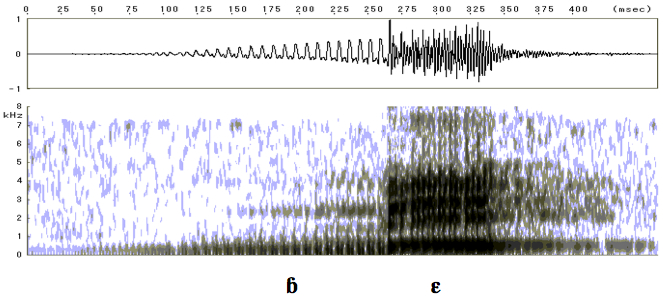
\includegraphics[width=\textwidth]{figures/mpiemoB}
\caption{Implosive [ɓ] in Mpiemo (\citet[172]{thornell2004})}
\label{Fig:mpiemo}
\end{figure}

\citet[312]{clements2002} describe the most salient features of implosives as being  \begin{quote} ``the absence of turbulence noise (in the form of burst or aspiration) at their release and the steady or rising amplitude of vocal fold vibration during the production of the constriction.'' \end{quote}

In Figure \ref{Fig:mpiemo}, the rising amplitude before the release is clearly seen in a typical cone shape, with voicing starting a good 150ms before the release. In contrast, Gyeli does not necessarily have the same type of amplitude increase, as shown in Figure \ref{Fig:Implb}. One could argue that instead the amplitude is steady, but then the release has more turbulence which is an indication for an egressive [b]. 

%change to png

\begin{figure} 
\centering
\includegraphics[width=\textwidth]{figures/GyeliB-Ada-mini}
\caption{Preglottalized and prevoiced [b] in Gyeli, speaker 1}
\label{Fig:Implb}
\end{figure}

Further,  the voicing onset starts with a glottal closure, marked by the circle in Figure \ref{Fig:Implb}. In fact, the manner of production of the word/stem initial egressive voiced stops in Gyeli involves the same places of articulation as implosives with a closure at the glottis, an increase of pressure in the oral cavity and finally a labial or alveolar release. The only difference is the movement of the glottis producing different kinds of airstreams. While in implosives the glottis usually moves downwards which causes an ingressive airstream, the airstream in Gyeli is always egressive with the glottis moving upwards. Evidence for this comes from the observation that speakers tend to expand their cheeks during prevoicing time/before release. This has also been noted by \citet{renaud76} for the Gyeli variety spoken in Bipindi. In order to expand the cheeks, the airflow has to be egressive.

The increase of airstream pressure in the oral cavity varies among speakers, as shown in Figure \ref{Fig:ImplbMama}. Here, the prevoicing before the release is not steady, but rising, however not in a regular way. And again, there is a good deal of turbulence noise during the release.

%change to png

\begin{figure} 
\centering
\includegraphics[width=\textwidth]{figures/GyeliB-Mama-mini}
\caption{Preglottalized and prevoiced [b] in Gyeli, speaker 2}
\label{Fig:ImplbMama}
\end{figure}

In summary, the perceived particularity in the production of stem initial [b] and [d] is related to pre-glottalization followed by a long prevoicing time. Speaker 1, for instance, has a prevoicing of 182ms in {\itshape bɛ̀ɛ̀} `shoulder' in Figure \ref{Fig:Implb}, speaker 2 has a prevoicing of 190ms in Figure \ref{Fig:ImplbMama}. During voicing, airstream pressure increases in the oral cavity which, in turn, leads to a more intense burst at the release.  The longer the voicing time, the potentially stronger is the burst at release. 

Closure duration of the voiced plosive does not depend on the quality of the following vowel, as explained in detail in \citet{grimm2019}. Instead, the duration depends on the speaking rate, the lexical or grammatical function of a morpheme or stem, and the position in the intonation phrase. Thus, closure duration is generally longer in careful speech, in initial position of lexical stems, and at the beginning of an intonation phrase. Vice versa, closure duration is shorter  in fast speech, in grammatical morphemes, and at the end of intonation phrases.


Also /g/ is prevoiced in word initial position, but lacks pre-glottalization in comparison to /b/ and /d/.  There are, however, not that many instances of a word initial /g/ which would allow for a more systematic investigation. In the lexeme {\itshape gɔ́lɛ̀} `gold', for instance, the prevoicing time amounts to 120ms. 

There are several ways to interpret these findings in relation to other Bantu A80 languages. Either, pre-glottalization followed by prevoicing of [b] and [d] could be areally more widespread, but it has not been recognized as such. Or, it is a special feature in Gyeli. It is even possible that these pre-glottalized stops are an imitation of sounds that are possibly implosives in neighboring languages. \citet{duke2014} observed in the Gyeli variety spoken around Bipindi, which is in contact with Kwasio and Basaa, that speakers mimick in a playful way sounds of neighboring languages. This happens, according to Duke, both in contact situations with non-Bagyeli, but also within the speech community in order to emphasize personal relations with other Gyeli community members with whom the individual may have spent some time with e.g.\ the Basaa. 







\subsubsection{Voicing of intervocalic stops}
\label{sec:Post-N}








\iffalse
\paragraph{Devoicing of stops after nasals}

Phonologically, both voiced and voiceless stops occur after nasals. Perceptually, their voicing status when prenasalized is, however, sometimes hard to distinguish. Even though postnasal voicing seems to be the more common process cross-linguistically, I argue that in Gyeli the rarer case of postnasal devoicing also occurs as allophonic variation, especially with labial and alveolar stops. This unusual behavior seems to be linked to pre-glottalization as discussed in \sectref{sec:Pre-glott}. Pre-glottalization in prenasalized environments is assimilated from an underlying [n'd] to either a double plosive [ntd] or an aspirated voiced plosive [ndh]. As a next assimilation step, postnasal stops are voiceless altogether. 

As discussed in the previous section, voiced stops in stem or word initial position tend to be pre-glottalized and show a relatively long prevoicing time, while they are clearly voiced in a non-aspirated way. In environments where they are prenasalized, pre-glottalization of the stop is assimilated and surfaces as one of various allophonic forms. One allophonic form is a double plosive which is the realization of /n'd/ $\rightarrow$ /ntd/. An example is given in Figure \ref{Fig:ntdalo} where an unaspirated voiced stop after a nasal involves a double closure after the nasal, first producing a voiceless and then a voiced stop. Instead of a glottal and then an alveolar closure, both stops are alveolar due to assimilation of the place of articulation. This happens within milliseconds and is acoustically not perceivable, but very clear from the wave sound in Figure \ref{Fig:ntdalo}.\footnote{Even though such examples are so rare in Gyeli that it is not clear whether a double closure after a nasal is contrastive, these instances are no recording or speech mistakes either. Speakers were consistent in their pronunciation and produce the double closure in every occurrence of the lexeme.}

\begin{figure} 
\centering
\includegraphics[width=\textwidth]{figures/ntdalo-mini}
\caption{Double plosive in /{\itshape ntdàlò}/ `tobacco'}
\label{Fig:ntdalo}
\end{figure}

The result of this assimilation is that on the surface, prenasalized voiced plosives undergo devoicing. If postnasal stops were subject to voicing rather than devoicing, one would expect that the distribution of the two stops was the inverse, namely the first stop being voiced and the second voiceless. The double stop in Figure \ref{Fig:ntdalo} with the voiceless plosive preceding the voiced one is an argument in support of the devoicing hypothesis.

Other allophonic forms of prenasalized voiced stops surface in the range of a voiced aspirated or devoiced, i.e.\ voiceless stop. These two possibilities occur in free variation and are represented for the lexeme /{\itshape ndɛ̀mɔ́}/ `dream (n.)' in Figures \ref{Fig:ndhemo} and \ref{Fig:ntemo}. Both tokens were produced by the same speaker. In Figure \ref{Fig:ndhemo}, the postnasal /d/ is aspirated so that voicing is interrupted between /d/ and the following vowel as seen in the fundamental frequency. 
Aspiration lasts for an average of 20ms comparable to voiceless stem or word intial stops. 
At the same time, the prevoicing time is much shorter than in non-prenasalized voiced stops.

\begin{figure} 
\centering
\includegraphics[width=\textwidth]{figures/ndhemo-mini}
\caption{Postnasal [d] with aspiration in /{\itshape ndɛ̀mɔ́}/ `dream (n.)'}
\label{Fig:ndhemo}
\end{figure}

\noindent In contrast, in Figure \ref{Fig:ntemo}, the lack of voicing during the stop release is clearly seen in the spectrogram.

\begin{figure} 
\centering
\includegraphics[width=\textwidth]{figures/ntemo-mini}
\caption{Devoiced postnasal [d] in /{\itshape ndɛ̀mɔ́}/ `dream (n.)'}
\label{Fig:ntemo}
\end{figure}

In summary, voiced stops that occur with prenasalization undergo assimilation and surface as one of three allophonic variants which reflect different stages of assimilatory development:
\begin{center}
/n'd/ $\rightarrow$ /ntd/ $\rightarrow$ /ndh/ $\rightarrow$ /nt/
\end{center}

Underlying pre-glottalization and prevoicing surface either as a double closure, as an aspirated voiced stop or as a voiceless stop under pre-nasalization. This assimilation chain ulitmately has the effect of stop devoicing after a nasal.
The decisive argument supporting the surface devoicing hypothesis rather than assuming that voiceless stops acquire voicing features from the preceding nasal is the following: In many cases, the underlying phonological form of a postnasal stop is known, i.e.\ whether the stop is underlyingly voiced or voiceless. Deverbal nominalization from verbs starting with a voiced plosive is a good test. In nominalization, the verb stem is preceded by a homorganic nasal. It becomes clear then that while a verb stem initial voiced stop is not aspirated, it is aspirated or even devoiced as a deverbal noun with aspiration being a feature of voiceless stops.



\fi





In intervocalic position, voiceless stops such as [p, t, k] are slightly voiced in fast speech. For instance, the noun /{\itshape ŋgàtà}/ `tied bundle' may surface as [{\itshape ŋgàdà}] just as /{\itshape fúkɛ̀}/ `driver ant' may be pronounced as [{\itshape fúgɛ̀}] (which then becomes a homonym with /{\itshape fúgɛ̀}/ `end'). 


\subsection{Consonant clusters}
\label{sec:CClusters}

Gyeli has a wide range of consonant sequences such as prenasalized consonants, labialized and palatalized stops, and consonant-fricative clusters. In many Bantu languages, these sounds are treated as single phonemic units. In Gyeli, I consider some of them as units, but some as clusters, i.e.\ sequences of phonemes. Following \citet[8]{guldemann2001}, I view clusters as ``a sequence of two consonantal constituents having phoneme status as independent segments which join together in one, more elaborate segment.''  In the following, I will present the various consonant clusters and explain how I delimit them from unit segments.

\subsubsection{Prenasalization}
\label{sec:Prenasa}

Gyeli has a variety of prenasals, mostly prenasalized obstruents, but also a few prenasalized glides and laterals.  Table \ref{Tab:Prenasalization} lists all nasal + consonant (NC) sequences. 
Every oral consonant in Gyeli that occurs stem initially can be prenasalized.

\begin{table} 
\centering
\begin{tabular}{l|llllll}
 \midrule
 & BL & LD & AL & PL & VL & LV \\  \midrule
Stops & {\itshape mp, {\bfseries mb}} & & {\itshape nt, {\bfseries nd}} &  & {\itshape ŋk, {\bfseries ŋg}} & {\itshape mgb} \\ 
Fricatives &  &  & {\itshape ns, nz} &  &  & \\ 
Affricates &  &  &  & {\itshape ntʃ, ndʒ} &  & \\ 
Lateral approximant & & & {\itshape nl} & & & \\
Glides & {\itshape mw} & & & {\itshape nj} & & \\
 \midrule
\end{tabular}
\caption{Prenasalized consonants}
\label{Tab:Prenasalization}
\end{table}


There are different ways to analyze the status of these prenasals which can either be treated as a single segment or as a sequence of segments, i.e.\ consonant clusters.  I argue that some NC occurrences form a segment unit, namely the ones in bold, while the others constitute clusters in Gyeli. The status distinction of NC segments into units versus sequences is primarily based on distributional properties, as I will explain in the following, while other diagnostics that are often used in Bantu studies to determine NC status can be ruled out as decisive criteria.  (The prenasalized labial velar is a marginal phenomenon and further discussed in \sectref{sec:LabV}.)

\citet{chacha2007} summarizes arguments that have been put forth in Bantu studies for and against treating prenasals as single segments. The main points of evidence concern homorganicity, duration, and syllabification. The author points out that ``similar gestural sequences in some languages should be treated as unitary segments, particularly if they occur in syllable-initial position''. As Table \ref{Tab:Prenasalization} shows, all NC segments are homorganic and, as I will show below, all occur in syllable-initial position. Therefore, homorganicity is not a criterion in Gyeli to distinguish NC units from NC sequences.  

Another putative diagnostic for NC segments as phonemic units concerns duration. It has been claimed that, if NC segments are units, 
 ``at the phonetic level, the prenasalized consonants have the same length as other consonantal segments'' (Chacha Mwita 2007: 61). According to \citet[183]{downing2005}, however, one cannot simply correlate the phonetic duration of prenasalized consonants with their segmental status. Both are language specific. In Gyeli, NC sequences seem to be longer than singleton segments, as (\ref{durationNCb}) and (\ref{durationNCk}) show.\footnote{Both (\ref{durationNCb}) and (\ref{durationNCk}) constitute single tokens and rather serve at giving an impression. For generalizations, a larger sample is needed. Since I do not consider duration as a decisive criterion in determining NC segment status, however, I do not investigate duration systematically at this point.}

\begin{exe} \ex \label{durationNCb}
\begin{tabular}{lll}
mɛ̀ `1\textsc{sg}' & $\rightarrow$ & [m] = 133ms\\
bɛ́ɛ̀ `shoulder' & $\rightarrow$ & [b] = 184ms \\
mbɛ̂ `door' &  $\rightarrow$ & [mb] = 255ms\\
\end{tabular}
\end{exe}

\noindent Longer duration of prenasalized in comparison to plain obstruents is more evident in prenasalized voiceless stops, as shown in (\ref{durationNCk}) since they lack the relatively long prevoicing time of voiced stops, as discussed in \sectref{sec:Allo}.

\begin{exe} \ex \label{durationNCk}
\begin{tabular}{lll}
ná `still (adv)' & $\rightarrow$ & [n] = 181ms\\
kà `catch' & $\rightarrow$ & [k] = 21ms \\
ŋká `line' &  $\rightarrow$ & [ŋk] = 200ms\\
\end{tabular}
\end{exe}

Another argument that is used in the discussion on the status of prenasals is syllabification. If the NC sequence belongs to the same syllable, it is usually viewed as a unit: 

\begin{quote} ``The fact that the units making up the prenasals usually find themselves in one syllable has been taken as proof that the consecutive consonants in a prenasal form a unit segment or one sound.''  (Chacha Mwita 2007: 62)
\end{quote}

This is true for all NC sequences in Gyeli since nasals are never syllabic, as shown in \sectref{sec:Syllable}. Gyeli has, synchronically, almost no nasal prefixes as would be common for Bantu languages. Instead, the nasal that most likely used to be a syllabic prefix has become frozen to the noun stem which becomes obvious in the plural classes which retain the nasal that occurs in the singular: {\itshape mbáálɔ́} `jaw' retains the /m/ in the plural class 4 {\itshape mimbáálɔ́} `jaws'. This suggests a closer liaison between nasal and obstruent.

This syllabification pattern is, however, not only the case for NC sequences such as /mb/, but also for those that are less typically viewed as single phonemic units, for example a nasal plus a lateral approximant [nl] as in {\itshape nlémò} `heart', {\itshape minlémò} `hearts'. While it is quite common for Bantu languages to have prenasalized obstruents as phonemic units, it is rather uncommon to have phonemic units of prenasalized lateral approximants. 

As an interim summary, the diagnostics of homorganicity, duration, and syllabification are either inconclusive (as far as duration is concerned) or seem to indicate a unit status of all NC sequences. The unit status is then based on homorganicity of all NC sequences and their occurrence within the same syllable. Considering the distribution of NC sequences, however, shows that there are differences between nasal + voiced stop sequences in contrast to other NC sequences, as illustrated in Table \ref{Tab:PreCons}. 


The table shows the distribution of NC sequences in nouns and verbs. For both nouns and verbs, different consonant positions in stems are represented. O1 stands for the onset of the first syllable in a stem, O2 for the second, and O3 for the third, irrespective of whether the onset is one single consonant or a cluster.

The numbers under O1, O2 and so on give total numbers of all NC sequences in this position. For instance, for O1 in nouns, 188 out of 855 nouns stems that have a consonantal onset in O1 start with an NC sequence. In contrast, 377 verb stems start with a consonant, but only 7 of them are prenasalized stops. The number of consonantal slots in O2 and O3 are decreasing because obviously they cannot be filled in mono- or bisyllabic stems.

\begin{table} 
\centering
\begin{tabular}{p{2cm}|lll|lll}
 \midrule
  &  \multicolumn{3}{c|}{\bfseries Nouns} &  \multicolumn{3}{c}{\bfseries Verbs} \\
{\bfseries NC}  & {\bfseries O1}  & {\bfseries O2}  & {\bfseries O3 }  &  {\bfseries O1} & {\bfseries O2}  & {\bfseries O3}   \\
   & 188/855 & 169/650 & 4/88 & 7/377 & 54/274 & -/76 \\  \midrule
         mp & 30 & 1 & -  & - & - & -  \\ 
          mb &  30    &   69  & - &   - & 25 &  - \\
         nt  &   26   &  1  &  - & 3 & - & -   \\
         nd  &    7  &  55  & 2 &  1 & 23 & -    \\ 
         ŋk   &   47   &  3  &  -  & - & - & - \\
         ŋg  &  24    & 39   & 2 & 1  & 6 & - \\
	mgb & 5    &  1   & - &     1  &  - & - \\
	ns	& 20  & -   &   -  & - &  - &  - \\
	nz	& 10 & - & - & - & - & - \\
         ntʃ	&  2 & - & - & - & - & - \\
         ndʒ	& 8 & 1 & - & 1 & - & - \\
         nl	& 9 & - & - & - & - & - \\
         mw	& 5 & - & - & - & - & - \\
 \midrule
\end{tabular}
\caption{Distribution of NC sequences}
\label{Tab:PreCons}
\end{table}

The distribution shows that all possible NC sequences occur in O1 of nouns while they are exceptions in O1 of verbs. This distribution can be explained by the noun class morphology, as already stated above: diachronically, the nasal was most likely a syllabic nasal prefix as it is common for many Bantu languages. Synchronically, the former nasal prefix has become frozen to the stem. 

Assuming this historic scenario, it is not surprising that NC sequences are almost absent in O1 position in verbs, with a few exceptions only. There are only a few instances where a verb starts with a prenasalized stop as in {\itshape ndà} `cross' or {\itshape ntɛ́gɛ̀lɛ̀} `disturb'. They are, however, restricted, not allowing prenasalized labials, and they are rather rare with only 6 occurrences in a database of 377 verbs, as shown in Table \ref{Tab:PreCons}.

There are, however, also NC sequences that occur in O2 of nouns and verbs (and exceptionally in O3 of nouns). They are restricted to voiced prenasalized stops.\footnote{Instances of voiceless nasal stops in O2 of nouns can be explained by reduplications.} These occurrences cannot be explained by diachronic noun class morphology, but suggest a different phonological status. Given the distributional differences, I propose a unit analysis for voiced prenasalized stops /mb/, /nd/, and /ŋg/ in Gyeli while I treat all other NC sequences as clusters. This holds the advantage of not artificially inflating the phoneme inventory while acknowledging the language's properties in terms of homorganicity and syllabification.



%The distribution shows that in general, prenasalized stops in C1 occur more in nouns than in verbs where they are negligible. It also shows that prenasalized stops in C2 position are restricted to voiced stops. (There are a few exceptions in the nouns, but that can be explained by either loan words or reduplication of the first syllable.) These prenasalized stops in C2 position cannot be explained by noun class morphology. They might be single phonemic units rather than consonant clusters, given that phonemic prenasalized stops are very common in Bantu languages and somehow to be expected.

%\begin{quote} ``Looking at any of the prenasals, one notices that the sonority hierarchy theory of syllable structure predicts that a syllable-initial prenasalized stop is unexpected'' (idem) \end{quote}

%\noindent According to theories of syllable structures, the greatest sonority is found in and towards the center of a syllable. In a syllable with a prenasalized onset, the sonority of the nasal at the margin would be higher than that of the following obstruent which would violate the sonority hierarchy. Following this hierarchy, a cluster analysis would only be justified if the preceding nasal constitutes a syllable by its own, as it is often the case with syllabic nasal noun class prefixes. 


%Further, in related languages, for instance in Abo (A40), the noun class prefix of some singular classes is a nasal. It is both syllabic and carries a floating L tone. This is not the case in Gyeli. These nasals are neither syllabic, nor do they carry any tone. Thus, unlike in Abo, no downstep phenomena, that may serve as a diagnostic for floating L tones, can be observed. 

%Assuming that the nasals preceding obstruents in the onset of noun's first syllables are frozen to the stem and derived from former syllabic noun class prefixes, it makes more sense to analyze these as a consonant cluster of nasal + obstruent. It seems less convincing to assume that two consonants merge into one forming a single phoneme rather than forming a cluster.

%Another argument in favor of a phonemic unit analysis of prenasals in Bantu is that ``the canonical Bantu syllable is of a CV form and therefore the prenasalized consonants are analyzed as simple consonant units'' (Chacha Mwita 2007: 62). Gyeli has other consonant clusters in addition to prenasals, as I will show in the following section. Labialized and palatalized obstruents as well as affricates are consonant clusters, too. So there is no need trying to simplify prenasalized obstruents for the sake of syllable onset structure. 





\subsubsection{Labialization and palatalization}
\label{sec:Labial}

Obstruents can occur in a labialized and/or palatalized form, i.e.\ the obstruent is followed by a labial or palatal glide. Both phenomena are specified in the lexicon rather than being phonological processes in Gyeli since their occurrence is not predictable from the (morpho-)phonological environment. According to \citet[55]{hyman2003}, ``The post-consonant glides [y] and [w] are typically derived from underlying vowels.'' Therefore, one would expect that certain vowels following a labialized or palatalized obstruent are disallowed.
 
 It turns out, however, that in Gyeli this is not the case. (\ref{bwn}) lists noun stems that start with /bw/, providing examples of different vowel heights. These examples contrast with (\ref{bn}) where /b/ is not labialized and followed by the same vowels. Therefore, labialization cannot be a phonological process that is determined by the consonant's phonological environment. Just like most NC sequences, I consider labialized and palatalized obstruents as consonant clusters rather than phonemic single units. This analysis is based on the fact that both consonants in the sequence can occur as independent phonemes on their own as well as distributional restrictions to first syllables.\footnote{Another possible analysis would be to assume a third category of complex consonants, in contrast to simple consonants and consonant clusters, as \citet{guldemann2001} proposes for !Xõo. While this is an elegant solution for !Xõo, it does not apply neatly to Gyeli. Introducing a third category rather moves the decision between unit and cluster analysis to another level.}

\begin{exe} 
\ex\label{bwn} /bw/ noun stem initial
\begin{xlist}
\ex bwímò `net hunting'
\ex bwújà `hundred'
\ex bwèdɔ̀wɔ̀ `taste'
\ex bwɔ̂ `brain'
\ex bwàndjá `disdain, adultery'
\end{xlist}
\end{exe}

\begin{exe} 
\ex\label{bn} /b/ noun stem initial
\begin{xlist}
\ex bíá `beer'
\ex búgɛ́ `tse tse fly (Glossina)'
\ex bé `well'
\ex bɔ́ndí `black colobus monkey'
\ex bàlándè `larva'
\end{xlist}
\end{exe}

The same is true for other obstruents and palatalization (for the sake of space,  I will not give examples for all of them). Another putative analysis would be that the glide is part of a diphthong.  Gyeli has four diphthongs: /uɔ/, /ua/, /ɔa/, /iɛ/ (see also \sectref{sec:Diph}). For instance, it would be possible that the diphthong /ua/ surface as [wa]. This, however, does not work out for two reasons. First, in that case we should only find labialization/palatalization with certain vowels--/w/ preceding /ɔ/ and /a/ and /j/ preceding /ɛ/. This is clearly not the case since these coarticulated consonants occur in front of any vowel, as shown above. Second, speakers pronounce diphthongs and labialized stops distinctly. This can be nicely illustrated with the minimal pair {\itshape bwɔ̂} `brain' vs. {\itshape búɔ̀} `mortar'.  


The fact that labialization and palatalization are not predictable realization rules in Gyeli is also seen in (near-)minimal pairs contrasting plain obstruents and obstruents + glide, as shown in (\ref{obsglidelab}) for labial glides and in (\ref{obsglidepal}) for palatal glides.

\begin{exe} \ex \label{obsglidelab}
{\bfseries bw}à `give birth' vs. {\bfseries b}â `marry' \\
{\bfseries kw}à `grind' vs. {\bfseries k}à `catch' \\
{\bfseries sw}áálɛ̀ `bone marrow' vs. {\bfseries s}áálɛ̀ `work (n.)'
\end{exe}

\begin{exe} \ex \label{obsglidepal}
{\bfseries dj}ɔ̀ `laugh' vs. {\bfseries d}ɔ̀ `negotiate' \\
{\bfseries kj}àlɛ `start an engine' vs. {\bfseries k}álɛ́ `sister' \\
lè-{\bfseries gj}ɔ́lɛ́ `bushbaby ({\itshape galago alleni})' vs. {\bfseries g}ɔ́lɛ̀ `gold'
\end{exe}



Labialized and palatalized obstruents basically only occur stem initially, as shown in Table \ref{Tab:LabCons}. Exceptions in second syllable onsets of noun stems are due to reducplication of the first syllable and loan words. Also, these sounds occur more frequently in nouns than in verbs. The most frequent ones are /bw/, /kw/, /dj/, /gj/.

\begin{table}
\centering
\begin{tabular}{l|lll|lll}
 \midrule
  &  \multicolumn{3}{c|}{\bfseries Nouns} &  \multicolumn{3}{c}{\bfseries Verbs} \\
 & {\bfseries O1} & {\bfseries O2} & {\bfseries O3} &  {\bfseries O1} & {\bfseries O2} & {\bfseries O3}   \\ 
                               & 59/855   & 2/650 & -/94 & 53/377 & -/274 &  -/76 \\  \midrule
{\bfseries labialized obstr.}  & & & & & &  \\
                        pw &     2 & 1  &  - & 1 & - & - \\
                        bw  &   12 &  - & - & 10 & - & -    \\
                        kw   & 10  &  -  & - & 9 & - & -   \\
                        gw	&   2  & -  & - & - & -  & -    \\ 
                        sw   &   3  & - & - &  2 & -  & -    \\  \midrule
{\bfseries palatalized stops}  &  &  &  & &    \\
                           pj & 1  & -  &  - & - & - & -    \\
                           dj &  11  & 1 & - &   12 & - & -   \\
                           kj &     1 & - & - &  2 & - & -  \\
                           gj &   17 & -  & - & 17 & - & -  \\
 \midrule
\end{tabular}
\caption{Labialized/palatalized consonants}
\label{Tab:LabCons}
\end{table}

Finally, labialized and palatalized obstruents can enter an even more complex consonant cluster by being preceded by a nasal. These complex sounds are, however, restricted to nouns. Table \ref{Tab:PrenCons} shows the distribution. Mostly, these complex sounds occur in O1 position, with the exception of /ndj/ which is more frequent in O2 than in O1.

\begin{table}
\centering
\begin{tabular}{l|lll}
 \midrule
{\bfseries pren. lab. stops}  & O1 & O2  & O3   \\
                         mpw &  1  &  &  \\
                         mbw &  5  & 1 &  \\
                         nkw &  6  &  &   \\
                         ngw  &  7  &  &   \\  \midrule
{\bfseries pren. palat. stops}  &  &  &   \\
                            ndj  &  2  & 13  &   \\ 
			    nkj  &  3 &  &   \\
                           ngj  &   8 & 1 &   \\    
 \midrule
\end{tabular}
\caption{Prenasalized and labialized/palatalized consonants in noun stems}
\label{Tab:PrenCons}
\end{table}

\noindent (\ref{prenstopglide}) opposes prenasal stops to prenasal stops + glide.

\begin{exe} \ex \label{prenstopglide}
{\bfseries mp}á `island' vs. {\bfseries mpw}á `bouillon' \\
{\bfseries nd}áwɔ̀ `house' vs. {\bfseries ndj}àwɔ̀ `chisel' \\
{\bfseries nk}ã̂ `guinea fowl' vs. {\bfseries nkj}ã̂ `scabies' 
\end{exe}







\subsubsection{Consonant-fricative clusters}
\label{sec:Affricates}

Consonant-fricative sequences are another series of consonant cluster in Gyeli. 
I propose to consider consonant-fricative sequences as clusters because i) their occurrence is highly restricted in terms of their distribution, unlike most other phonemic units, and ii) a unit analysis would be typologically uncommon for these sequences. Treating all of them as phonemic units would again artifically expand the phoneme inventory. Further, a cluster analysis is in line with the treatment of prenasal and labialized/palatalized consonant clusters.

Most of the consonant-fricative clusters consist of a stop + fricative, but there are also lateral + fricative sequences, as Table \ref{Tab:Aff} shows. All of them are restricted to the onset of the first syllable, both in noun and verb stems. The only exception of an occurrence of /bv/ in O2 in the table is a reduplication of the first syllable.

%Gyeli has a series of homorganic affricates: [pf], [bv], [ts], [dʒ].\footnote{Note that I will represent [dʒ] in the orthography according to Bantu tradition as {\itshape dj}.} /ts/ is also realized as /tʃ/ sometimes, depending on the speaker. Table \ref{Tab:Aff} shows the frequency and distribution of affricates.

\begin{table}[!h]
\centering
\begin{tabular}{l|lll|lll}
 \midrule
Consonant-  &  \multicolumn{3}{c|}{\bfseries Nouns} &  \multicolumn{3}{c}{\bfseries Verbs} \\
fricative & {\bfseries O1} & {\bfseries O2} & {\bfseries O3} &  {\bfseries O1} & {\bfseries O2} & {\bfseries O3}   \\ 
 sequence             & 40/855   & 1/650 & -/94 & 27/377 & -/275 &  -/76 \\  \midrule
%{\bfseries Homorganic affricates}  & {\bfseries 37} &   &    & {\bfseries 33} &  &  \\
			   pf       &  6  & -  &  - & 5 & - & - \\
			   bv        &  6  &  1  &  - & 6 & - & - \\
			 %  ts/tʃ    &  16     & -   &   - & 9 & - & -\\
			  % dʒ       &   9   &  -  &  - & 13 & - & -  \\
%{\bfseries Heterorganic affricates}  & {\bfseries 26} &   &  & {\bfseries 14} & &   \\
                             tf   &  6  & -  & - & 5 & - & - \\
                             dv   & 4   & -  &  - & 5 & - & - \\
                            kf      & 16  & -  & - & 4 & - & -  \\ 
                            lv      & 2  & -  & - & 2 & - & -  \\  \midrule
{\bfseries pren. stop-fric.}  & {\bfseries 24} &  & & & &    \\
                            mbv   & 8  & -  &  -  & - & - & -  \\
			    ndv    & 2   & -  & -  & - & - & -  \\
                           nkf    &  5  & -  &  -  & - & - & -  \\
                           ngv   &   9  & -  & - & - & - & -  \\        
 \midrule
\end{tabular}
\caption{Distribution of consonant-fricative clusters}
\label{Tab:Aff}
\end{table}

%In addition to these homorganic affricates, there seem to be a few heterorganic ones: [tf], [dv], [kf]. 
All consonant-fricative clusters are relatively rare, [kf] being the most frequent sequence type, at least in noun stems.\footnote{An observation with respect to the closest related language Mabi: Mabi does not have the phoneme [kf], but rather uses [pf] as in Mabi {\itshape pfúmá} `chief' where the Bagyeli say {\itshape kfúmá}. It is not clear, however, if this is a regular sound correspondence since Gyeli uses both (non-allophonic) sequences [pf] and [kf].} In contrast, /lv/ sequences are the least frequent.


Some of the stop-fricative clusters appear also prenasalized, as shown in Table \ref{Tab:Aff}. Prenasalization is, however, restricted to a subset of consonant-fricative clusters in noun stems, including prenasalization of /bv/, /dv/, /kf/, and /gv/. /gv/ as voiced counterpart to /kf/ only occurs if a nasal precedes it. Prenasalized consonant-fricative clusters do not occur in verbs.

%If one agrees that the prenasalized affricates in nouns are a consonant cluster of nasal + affricate and adds their numbers to the general numbers of homorganic and heterorganic affricates, the two latter are equally frequent in nouns, while homorganic affricates occur double as often in verb stem onsets than heterorganic ones.

Consonant-fricative clusters are further restricted in their distribution in that they only occur before the high vowel /u/.  This makes it likely to assume a realization rule of affrication, as for instance \citet[26]{velde2008} describes for Eton. There is, however, no complementary distribution or conditioning of the fricative cluster occurrence with respect to plain consonants. Their occurrence is not predictable from any rules, as the (near-)minimal pairs in (\ref{aff}) show. 

\begin{exe} \ex \label{aff}
{\bfseries bv}úlɛ̀ `Bulu person' vs. {\bfseries b}úlɛ `burst' \\
{\bfseries tf}údɛ́ `bump' vs. {\bfseries t}údɛ̀ `tumor' \\
{\bfseries kf}údɛ `cover' vs. {\bfseries k}údɛ́ `skin' \\
{\bfseries lv}úmɔ́ `maggot' vs. {\bfseries l}ùmɔ́ `yellow fever mosquito' 
%{\bfseries tʃ}ìì `live' vs. {\bfseries t}íì `get going' \\
%{\bfseries dʒ}íyɛ `burn (intr.)' vs. {\bfseries d}íyɛ̀ `expensive' 
\end{exe}

\noindent All initial consonants are followed by the same high back vowel [u]. Speakers are aware of the difference and correct me if I pronounce it wrong either way.

While ruling out a realization rule of affrication, one could still assume that stop-fricative clusters should be viewed as either homorganic or heterorganic affricates. An argument in favor of this hypothesis is that the affricates /tʃ/ and /dʒ/ are equally restricted in their distribution: they only occur in first syllables of noun and verb stems and they precede only the vowel /i/.

There are several reasons, however, why I treat affricates /tʃ/ and /dʒ/ as phonemic units which are distinct from consonant-fricative clusters. First, clusters are {\itshape per definitionem} comprised of two consonantal constituents which have independent phonemic status. While this is true for the consonant-fricative clusters, it does not hold for the affricates: /ʃ/ and /ʒ/ are not independent phonemes in Gyeli. Second, the affricates are better explained within the system as filling a slot in the palatal series, as also suggested by \citet[335]{cheucle2014} for other A80 languages. She further points out that affricates are viewed as phonemic units in other A80 languages. It also seems to be more systematic to group the clusters as distinct from the affricates since they differ in the type of fricative. While consonant-fricative clusters always involve a labiodental fricative, the affricates /tʃ/ and /dʒ/ involve a palatal fricative.









\subsection{Phonotactics}
\label{sec:Phonotact}


In this section, I lay out the phonotactics, i.e.\ distribution and frequency, of consonants comparing noun and verb stems. The basis for my analysis is a database of 875 noun and 377 verb stems.\footnote{Note that there is a much higher number of verb forms, namely derived verbs that take verb extensions. I consider, however, only synchronically non-derived verb stems. If, on the other hand, a verb stem has an applicative extension {\itshape -ɛlɛ}, but synchronically there is no basic verb stem (anymore), I consider this applicative form in my analysis. For more information on verbs and verb extensions, see \sectref{sec:V}.} 

Consonants only occur in syllable onset positions, and almost never as codas (with the exception of a few nasals). Noun stems can have up to four syllables, verb stems up to three. (For more detailed information on syllable structure, see \sectref{sec:Syllable}.) Tables \ref{Tab:PhonotactN} and \ref{Tab:PhonotactV} reflect the syllable structure for the potential occurrence of consonants in nouns and verbs, respectively. Thus, O1 (onset 1), for instance, stands for the stem initial consonant slot, O2 (onset 2) for the consonant slot in the second syllable and so on. I prefer to refer to onsets rather than to C (consonant) because these slots can be filled by multiple consonant, i.e.\ consonant clusters as discussed in \sectref{sec:CClusters}.

The number following O1, O2, and so on refers to the number of onsets. For example, out of 875 noun stems, 855 have an onset in their first syllable, while there are only 650 onsets  in the slot O2, and only 94 in O3. There are two reasons why the number does not match the total number of noun/verb stems. First, there are a few loan words which do not have a consonantal onset, for instance {\itshape èsã̂s} `fuel'. Second, the numbers are decreasing for slots O2, O3 (and O4) because noun and verb stems have different syllable lengths. Monosyllabic stems obviously do not have an O2 slot, so the potential number of O2 occurrences is smaller than for O1.

%See Table \ref{Tab:PhonStat} in \sectref{sec:Syllable}

\begin{table} 
\centering
\begin{tabular}{l|llll}
 \midrule
 & O1 (855) & O2 (650) &  O3 (88)   & O4 (6) \\  \midrule
{\bfseries Stops}  & {\bfseries 205 (24\%)} & {\bfseries 138 (21.2\%)}  & {\bfseries 14 (15.9\%)} &   {\bfseries 1 (16.6\%)}  \\ 
        p &  36  & 4  &  -  & - \\ 
         b  &  54   &  28  &  2  & - \\
          t  &   31  &  10  &  1 &  - \\
        d   &   19 &   43 &  7  & - \\
         k  &   63  &   15  & 3  & - \\
          g &   2  &  25  & 6 & 1 \\
         '  &   -   & 13   & -  & - \\  \midrule
{\bfseries Affricates}  & {\bfseries 25 (2.9\%)}  & - & - & - \\ 
	tʃ &  16   &  -  & - &  -\\
	dʒ &  9  &  -  & -   & - \\   \midrule
{\bfseries Fricatives}  & {\bfseries 97 (11.3\%)} & {\bfseries 48 (7.4\%)} & {\bfseries 9 (10.2\%)} &  {\bfseries 1 (16.6\%)}  \\
           f& 11 &  2  & 1 & - \\ 
           v &  25   &  5  & -  & - \\ 
          s  &  58    &  36  & 7  & - \\
         z  &  3   &  5  & 1  &  1 \\  \midrule
{\bfseries Nasals}  & {\bfseries 56 (6.5\%)} & {\bfseries 92 (14.2\%)}  & {\bfseries 17 (19.3\%)}  &  {\bfseries 1 (16.6\%)}  \\
         m & 24     &  60   & 5 & - \\ 
         n  &   7   &   28  & 12  & 1 \\
         ɲ  &  25    & 4   & - & -  \\  \midrule
{\bfseries Glides}  & {\bfseries 67 (7.8\%)} & {\bfseries 176 (27.1\%)}  & {\bfseries 40 (45.5\%)} &  {\bfseries 3 (50\%)}  \\
           l &   29  &  125  &  30 &  2 \\
           w &   22  &   30  &  9 &  - \\
           j  &  16   &  21  & 1  & 1 \\  \midrule
{\bfseries Pren. stops}  & {\bfseries 61 (7.1\%)}   & {\bfseries 163 (25.1\%)} & {\bfseries 4 (4.5\%)} & - \\
	mb    & 30 & 69 & - & - \\
	nd     & 7 & 55 & 2 & - \\
	ŋg	& 24  & 39 & 2 & - \\  \midrule
{\bfseries Total} & {\bfseries 59.6\%} & {\bfseries 95\%} & {\bfseries 89.7\%} & {\bfseries 100\%}   \\  \midrule	
\end{tabular}
\caption{Phonotactics of Phonemic Consonants in Noun Stems}
\label{Tab:PhonotactN}
\end{table}

Tables \ref{Tab:PhonotactN} and \ref{Tab:PhonotactV} show the frequency and distribution of all 22 phonemic consonants in Gyeli noun and verb stems. Allophones are included with their respective phoneme. For instance, occurrences of intervocalic [β] are subsumed unter the phoneme /b/. The bold numbers in the rows of `stops', `affricates,  `fricatives', `nasals', `glides', and `prenasalized stops' show the sums of their respective single phonemes. For example, 56 is the number of all occurrences of /m/, /n/, /ɲ/ taken together in O1 noun stem position. This is 6.5\% of all noun stem onsets which means that nasals are relatively rare in noun stem initial position.
The percentages at the bottom under `Total' sum up all phonemic unit instances in a particular slot. For O1 in noun stems, for instance, only 59.6\% have a phonemic unit onset. The other 40\% constitute consonant clusters.


\begin{table} 
\centering
\begin{tabular}{l|lll}
 \midrule
 & O1 (377) & O2 (274) &  O3 (76)    \\  \midrule
{\bfseries Stops}  & {\bfseries 129 (32.6\%)} & {\bfseries 66 (24.1\%)}  & {\bfseries 9 (11.8\%)}   \\ 
        p & 20  & -  &  -   \\ 
         b  & 34   & 17 & 1    \\
          t  &  22   &  4  &  1 \\
        d   & 7   &  19  &  3  \\
         k  &  39   &  7   &  -  \\
          g &  1   & 16  & 4  \\
         '  &   -   & 3   & -   \\  \midrule
{\bfseries Affricates}  & {\bfseries 22 (5.8\%)}  & - & - \\ 
	tʃ &    9 &  -  & - \\
	dʒ &  13  &  -  & -    \\   \midrule
{\bfseries Fricatives}  & {\bfseries 65 (17.2\%)} & {\bfseries 20 (7.3\%)} & {\bfseries 10 (13.2\%)}  \\
           f & 4 &  -  &  - \\ 
           v &  24  &  -  & -  \\ 
          s  &  37    & 20   &  10 \\
         z  &  -  &  -  &  - \\  \midrule
{\bfseries Nasals}  & {\bfseries 26 (6.9\%)} & {\bfseries 51 (18.6\%)}  & {\bfseries  5 (6.6\%)}   \\
         m &  8  &  37   &  - \\ 
         n  &  4   &  14   & 5 \\
         ɲ  &  14  &  -  &  - \\  \midrule
{\bfseries Glides}  & {\bfseries 45 (11.9\%)} & {\bfseries 82 (29.9\%)}  & {\bfseries  51 (67.1\%)}  \\
           l &   31  & 48   &  44 \\
           w & 10   &   17  &  7 \\
           j  &  4  & 17  & -  \\  \midrule	
{\bfseries Pren. stops}  & {\bfseries 2 (.5\%)}   & {\bfseries 54  (19.7\%)} & -  \\
	mb   & - & 25 & -  \\
	nd    & 1 & 23 &  - \\
	ŋg 	& 1  & 6  & -  \\  \midrule
{\bfseries Total} & {\bfseries 74.9\%} & {\bfseries 99.6\%} & {\bfseries 98.7\%} \\  \midrule
\end{tabular}
\caption{Phonotactics of Phonemic Consonants in Verb Stems}
\label{Tab:PhonotactV}
\end{table}

In both noun and verb stems, stops and fricatives generally occur stem initially, but their occurrences decrease in O2 and O3. The contrary is the case for nasals and glides: their occurrences are more numerous in O2 and O3 while they are rather rare stem initially.\footnote{O4 in noun stems should not be counted in these generalizations since there are only 6 occurrences anyway so that their numbers are not representative. The same may be true for O3 in verb stems.} 

In terms of voicing, some plosives are more frequent in stem initial position, such as /t/ and /k/ which are more frequent in O1 than their counterparts /d/ and /g/, whereas in O2 the inverse is the case. This holds for both noun and verb stems. The situation is different for bilabial stops where the voiced /b/ is more frequent in any position; in verb stems, /p/ only occurs in O1.

This voicing distribution is not true for fricatives in general. /v/ is more frequent than /f/ in O1 and O2 in both noun and verb stems. For the alveolar fricatives, though, the voiceless /s/ is always more frequent than voiced /z/. Interestingly, /z/ does not occur in verbs at all. Further, /s/ is the only fricative in verb stems that occurs in other positions than O1.

As to nasals, /m/ is more frequent than /n/ in both nouns and verbs. These two phonemes mostly occur in O2. In contrast, /ɲ/ is only found in in O1 in verb stems which is also generally true for nouns. The four occurrences  of /ɲ/ in O2 of nouns can be explained by reduplication and loan words.

Similar to nasals, glides are also more frequent in O2 than in O1. /l/ is the most frequently used phoneme in this position. As to the semi-vowels, /w/ is generally more frequent than /j/ in O1 and for noun stems also in O2, while the distrubution of /w/ and /j/ is equal for O2 in verbs.

Comparable to the voiced alveolar stop /d/ and the nasals /m/ and /n/, prenasalized stops are more frequent in O2 than in O1 position. This is true for both noun and verb stems. Another exceptional distribution concerns affricates which only occur in O1 position, but never stem medially. 

The tables also show that verb stems generally have a higher percentage of plain consonants which, in turn means, that consonant clusters are more common in noun stems. About 40\% of noun stem initial onsets consist of clusters, while for verbs only about a quarter of the stems begin with a sequence of consonants. The trend also holds in onsets of second and third syllables. For O2, about 95\% have phonemic units in nouns while it is 99.6\% in verbs.

As already discussed in \sectref{sec:CClusters}, most consonant clusters occur stem initially, with the exception of a few prenasalized stops which also occur in O2. Table \ref{Tab:CClust} summarizes the distribution of consonant clusters in O1 and O2\footnote{Consonant clusters do not generally occur in O3 or O4.}, contrasting noun and verb stems. Since detailed information was already given in the respective discussions of single consonant cluster types, I only list types of sequences here.\footnote{The various types of sequences include the following consonant clusters: prenasalized obstruents: [mp, nt, ŋk, mgb, ns, nz, nl, mw]; Labialized onstruents: [pw, bw, kw, gw, sw]; Palatalized onstruents: [pj, dj, kj, gj]; Stop-fricative cluster: [pf, bv, tf, dv, kf]. Further,  labial velars are subsumed under prenasalized obstruents since their only occurrence is in a cluster [mgb].}

\begin{table} 
\centering
\begin{tabular}{lll|ll}
 \midrule

 & \multicolumn{2}{l|}{{\bfseries Nouns}}  & \multicolumn{2}{l}{{\bfseries Verbs}}   \\
 & \multicolumn{2}{l|}{(855 total)}  & \multicolumn{2}{l}{(377 total)}   \\  \midrule
Cluster type & O1 & O2 & O1 & O2 \\  \midrule
Pren. obstr. & 208 (24.3\%) & 5 (.8\%) & 4 (1.1\%) & - \\
Lab. obstr. & 29 (3.4\%) & 1 (.2\%)  & 22 (5.8\%) & - \\
Pal. obstr. & 30 (3.5\%) & 1 (.2\%) & 31 (8.2\%) & - \\
Stop-fric. cl. & 40 (4.7\%) & - & 27 (7.2\%) & - \\  \midrule
{\bfseries Total} & {\bfseries 35.9\%} & {\bfseries 1.2\%} & {\bfseries 22.3\%} & - \\  \midrule
\end{tabular}
\caption{Phonotactics of Consonants Clusters in Noun and Verb Stems}
\label{Tab:CClust}
\end{table}

It is remarkable that prenasalized obstruents mostly occur stem initially in nouns while they rarely occur in O1 in verb stems. They do occur in O2 in verbs, but they are still more frequent in the same position in nouns. Prenasalized stops are basically the only consonant clusters that occur stem medially. The exceptional couple of labialized and palatalized obstruents in noun O2 can be explained by reduplication of the stem's first syllable or by loan words.

While prenasalized clusters are more frequent in noun stems, labialized/palatalized obstruents as well as affricates are more frequent in verb stems. Summing up all consonant clusters, almost 40\% of noun stems start with a consonant sequence while only 28\% of verb stems do so. This trend also holds for O2 with about 26\% in nouns and 18\% in verbs. These figures reflect what has already been stated for the distribution of plain phonemes which are more often found in verb than in noun stems. 





\section{Vowels}
\label{sec:Vowels}

Gyeli has seven contrastive vowels. In addition, the language has a range of diphthongs, as well as contrastive vowel length and nasalized vowels. I will discuss each of these in turn, starting with presenting `plain', i.e.\ short, oral vowels.

\subsection{Plain vowels}
\label{sec:CardVowels}

 Figure \ref{Fig:Vowels} shows the seven plain vowels /i/, /u/, /e/, /o/, /ɛ/, /ɔ/, /a/.

\begin{figure} 
\centering
\begin{tikzpicture}[scale=3]
\large
\tikzset{
    vowel/.style={fill=white, anchor=mid, text depth=0ex, text height=1ex},
    dot/.style={circle,fill=black,minimum size=0.4ex,inner sep=0pt,outer sep=-1pt},
}
\coordinate (hf) at (0,2); % high front
\coordinate (hb) at (2,2); % high back
\coordinate (lf) at (1,0); % low front
\coordinate (lb) at (2,0); % low back
\def\V(#1,#2){barycentric cs:hf={(3-#1)*(2-#2)},hb={(3-#1)*#2},lf={#1*(2-#2)},lb={#1*#2}}

% Draw the horizontal lines first.
\draw (\V(0,0)) -- (\V(0,2));
\draw (\V(1,0)) -- (\V(1,2));
\draw (\V(2,0)) -- (\V(2,2));
\draw (\V(3,0)) -- (\V(3,2));

% Place all the unrounded-rounded pairs next, on top of the horizontal lines.
\path (\V(0,0))     node[vowel, left] {i}  node[dot] {};
%\path (\V(0,1))     node[vowel, left] {ɨ} node[vowel, right] {ʉ} node[dot] {};
\path (\V(0,2))      node[vowel, right] {u} node[dot] {};
%\path (\V(0.5,0.4)) node[vowel, left] {ɪ} node[vowel, right] {ʏ} node[dot] {};
%\path (\V(0.5,1.6)) node[vowel, left] { } node[vowel, right] {ʊ} node[dot] {};
\path (\V(1,0))     node[vowel, left] {e}  node[dot] {};
%\path (\V(1,1))     node[vowel, left] {ɘ} node[vowel, right] {ɵ} node[dot] {};
\path (\V(1,2))      node[vowel, right] {o} node[dot] {};
\path (\V(2,0))     node[vowel, left] {ɛ}  node[dot] {};
%\path (\V(2,1))     node[vowel, left] {ɜ} node[vowel, right] {ɞ} node[dot] {};
\path (\V(2,2))      node[vowel, right] {ɔ} node[dot] {};
%\path (\V(2.5,0))   node[vowel, left] {æ} node[vowel, right] { } node[   ] {};
\path (\V(3,0))     node[vowel, left] {a}  node[dot] {};
%\path (\V(3,2))     node[vowel, left] {ɑ} node[vowel, right] {ɒ} node[dot] {};

% Draw the vertical lines.
\draw (\V(0,0)) -- (\V(3,0));
\draw (\V(0,1)) -- (\V(3,1));
\draw (\V(0,2)) -- (\V(3,2));

% Place the unpaired symbols last, on top of the vertical lines.
%\path (\V(1.5,1))   node[vowel]       {ə};
%\path (\V(2.5,1))   node[vowel]       {ɐ};
\end{tikzpicture}
\caption{Plain vowels in Gyeli}
\label{Fig:Vowels}
\end{figure}

(\ref{vowels}) provides (near-)minimal pairs of all seven vowels, demonstrating their functional contrast.


\begin{exe} \ex \label{vowels}
\begin{tabular}{llll}
{\bfseries /i/ vs. /u/} & /k{\bfseries ì}ndá/ `sugar ant' & vs. &  /k{\bfseries ù}ndá/ `shoe' \\
{\bfseries /u/ vs. /o/} &  /k{\bfseries ù}lɛ/ `borrow'  & vs. & /k{\bfseries ò}lɛ/ `help' \\
{\bfseries /e/ vs. /ɛ/} & /l{\bfseries é}/ `tree' & vs. & /l{\bfseries ɛ́}/ `glass' \\
{\bfseries /o/ vs. /ɛ/} & /k{\bfseries ò}lɛ/ `help' & vs. &  /k{\bfseries ɛ̀}lɛ/ `hang' \\
{\bfseries /ɛ/ vs. /i/} & /l{\bfseries ɛ̀}bɛlɛ/ `follow' & vs. & /l{\bfseries í}bɛlɛ/ `show' \\
{\bfseries /ɔ/ vs. /ɛ/} &  /kámb{\bfseries ɔ}/ `chew' & vs. &  /kámb{\bfseries ɛ̀}/ `weaver ant' \\
{\bfseries /a/ vs. /ɛ/} & /kìj{\bfseries a}/ `give' & vs. &  /kìj{\bfseries ɛ}/ `try' \\
{\bfseries /o/ vs. /ɔ/} & /béd{\bfseries o}/ `ferment' & vs. & /béd{\bfseries ɔ}/ `go up' \\
{\bfseries /i/ vs. /a/} & /wùs{\bfseries i}/ `sprout' & vs.  & /wùs{\bfseries a}/ `forget' \\
\end{tabular}
\end{exe}

\subsubsection{Vowel space} 

The Gyeli vowel system is the same as what  \citet[389]{cheucle2014} reconstructs for Proto-A80. Synchronically, Bantu A80 languages differ in the number of phonemic vowels and vowel quality as described by \citet[324]{cheucle2014}. According to her summary of the literature, most of these languages have six phonemic vowels /i, e, ɛ, a, o, u/, while Shiwa and Kwasio only have a five-vowel-system /i, e, a, o, u/ where /e/ and /o/ are variants of /ɛ/ and /ɔ/, respectively. This special status of /e/ and /o/ is also seen in Gyeli. Even though these two vowels have a constrastive function as shown in (\ref{vowels}) and therefore must be considered phonemes, /e/ and /o/ differ from the other vowels in two respects. First, they are significantly less frequent than other vowels, as will be shown in, for instance, Tables \ref{Tab:MonoV} and \ref{Tab:PhonoDiV} in the discussion of vowel phonotactics. Second, the plotting of the Gyeli vowel space in Figure \ref{Fig:plot} shows that both /e/ and /o/ are cramped between /i/ and /ɛ/ and /u/ and /ɔ/, respectively.\footnote{The vowel chart was plotted from 233 vowel tokens taken from two male speakers. I used a Praat script to measure F1 and F2. For extreme outliers I corrected the fundamental frequencies manually. These cases all concerned word final vowels. Many thanks to Joyce McDonough and Murray Schellenberg for their help with this.} 

\begin{figure} 
\centering
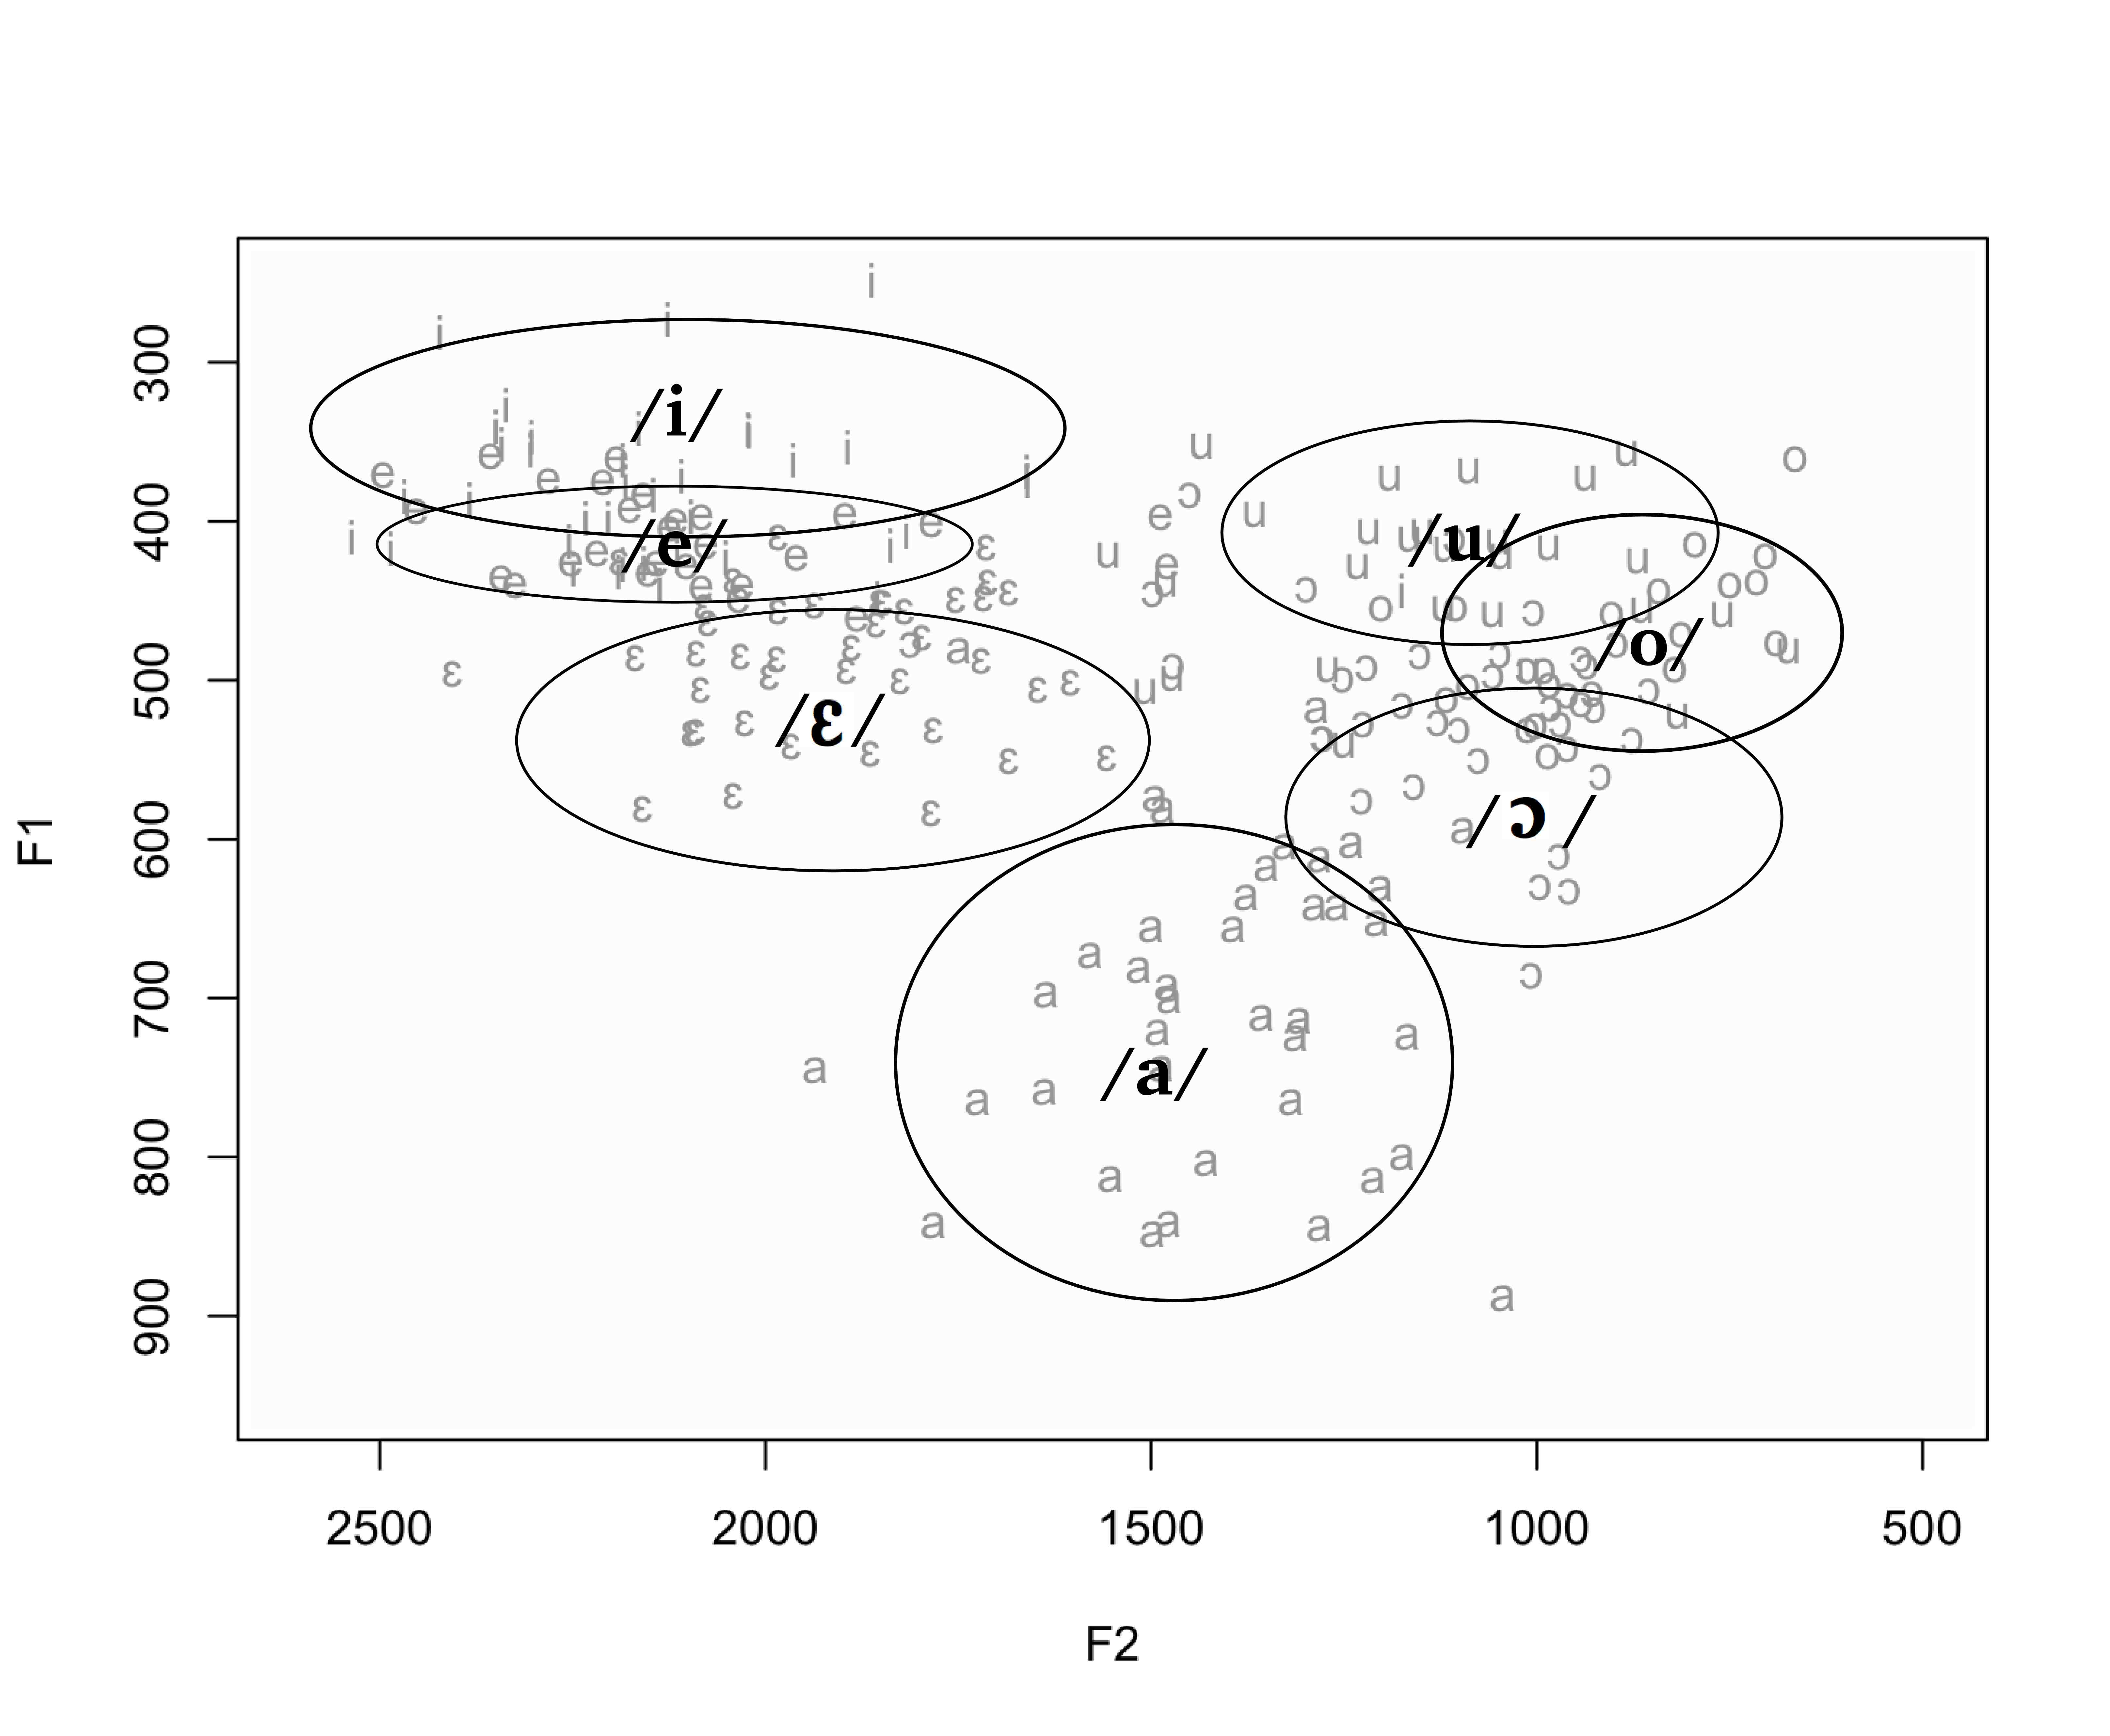
\includegraphics[width=\textwidth]{figures/Vowel-plot-mini}
\caption{Vowel plot}
\label{Fig:plot}
\end{figure}

While a 7-vowel system is the norm in Bantu languages, the Gyeli vowel space differs from what is generally expected for Bantu languages. \citet[18]{maddieson2003a} notes that 
\begin{quote}
``Bantu vowel inventories, both five- and seven-vowel-systems, are split between those which are similar to global norms in their spacing [i.e.\ evenly distributed] and those in which the vowels are atypically crowded in the higher part of the vowel space.''
\end{quote}
Vowels are neither evenly distributed in the vowel space in Gyeli, nor are the vowels atypically cramped in the higher part. Maddieson's example of a 7-vowel system, with atypical crowding in the higher part, still differs from Gyeli in that the high and mid vowels are relatively evenly spaced with respect to one another while there is a relatively large space between the mid vowels and /a/. What seems to be atypical in Gyeli is that /e/ and /o/ are tightly wedged between /i/ and /ɛ/ and /u/ and /ɔ/, respectively. With the exceptions of /e/ and /o/, the other five vowels are fairly evenly distributed.

 The Gyeli system is very similar to the one of Mpiemo that \citet[167]{thornell2004} describe. Also in Mpiemo, /i/ and /e/, and /u/ and /o/ are very close together. Further, both languages have a common relation of the spacing between the lower mid vowels /ɛ/ and /ɔ/ to /a/, the mid vowels ranging at on average around 500 Hz in F1 and /a/ at a mean of about 730 Hz. There are, however, differences concerning mostly F2 for the high vowels which range at under 1000 Hz in Gyeli, but slightly under 700 Hz in Mpiemo. 


\subsubsection{Vowel phonotactics} 

In terms of frequency and distribution of vowels, a general observation is that high vowels /i, u/ occur more in first syllables of both verb and noun stems while lower mid vowels /ɛ, ɔ/ and low vowel /a/ are more frequent in second syllables. This becomes obvious when comparing plain vowels in noun and verb stems of different syllable length which are summarized in Table \ref{Tab:CardV}. This concerns only plain vowels and does not represent general syllable distribution, as discussed in \sectref{sec:Syllable}.


\begin{table} 
\centering
\begin{tabular}{l|ll}
& Noun stems &   Verb stems \\  \midrule
$\sigma$    & 108  &    39 \\
$\sigma$ $\sigma$  & 508 & 205 \\
$\sigma$ $\sigma$ $\sigma$ & 93 &  76 \\  \midrule
\end{tabular}
\caption{Frequency of plain vowels in noun and verb stems}
\label{Tab:CardV}
\end{table}

\noindent  Bisyllabic stems are most frequent for both noun and verb stems, as Table \ref{Tab:CardV} shows. In contrast, it is more frequent for nouns to have plain vowels with monosyllabic than with trisyllabic stems, while the inverse is the case for verbs.

\begin{table} 
\centering
\begin{tabular}{l|ll}
Vowel & Noun stems & Verb stems \\  \midrule
i &  	14 (13\%) &  4 (10.3\%) \\
u & 	18 (16.6\%) & 4 (10.3\%) \\
e & 	3 (2.7\%) &  2 (5.1\%) \\
o & 	3 (2.7\%) & - \\ 
ɛ &  	18 (16.6\%) & 11 (28.2\%) \\
ɔ & 	18 (16.6\%) & 6 (15.4\%) \\ 
a  & 	34 (31.5\%) & 12 (30.8\%) \\
\end{tabular}
\caption{Distribution of plain vowels in monosyllabic stems}
\label{Tab:MonoV}
\end{table}

Table \ref{Tab:MonoV} shows the frequency of the various plain vowels in monosyllabic noun stems, contrasting them with verb stems. While the high back vowel /u/ occurs slightly more often than its front counterpart /i/ in noun stems, the distribution of these two high vowels is more equal in verbs. Mid vowels /e, o/ are rare in both nouns and verbs. /o/ is even completely absent in monosyllabic verb stems.\footnote{Despite this low frequency of mid vowels, they can still not be subsumed under either higher or lower vowels since there are minimal pairs that prove their contrastive function.} Also, in both noun and verb stems, the most frequent plain vowel is /a/ with over 30\%.

Comparing plain vowel distribution in bisyllabic noun and verb stems shows that the occurrence of vowels is more restricted in verb than in noun stems, as shown in Tables \ref{Tab:PhonoDiN} and \ref{Tab:PhonoDiV}. For both, there is a tendency that high vowels occur more frequently in the first than in the second syllable. In verb stems, though, high vowels systematically do not occur at all in the second syllable.\footnote{The two instances of /i/ in the second verb stem syllable shown in Table \ref{Tab:PhonoDiV} are most likely loan words.}

\begin{table} 
\centering
\scalebox{0.85}{
\begin{tabular}{l|lllllll|p{1cm}l}
\backslashbox{$\sigma$1 $\downarrow$}{$\sigma$2 $\rightarrow$} &	i &  	u & 	e & 	o & 	ɛ & 	ɔ & 	a & 	Total $\sigma$1 & \% \\  \midrule
i & 	23 & 11 &  - &  3 &  7 &  	29 &  15 &  88 &  (17.3) \\
u & 	11 & 15 & 5 &  6 &  	43 &  37 &  29 &  146 & (28.7) \\
e & 	1 & 	- & 	1 & 	4 & 	3 & 	2 & 	1 & 	12 & (2.4) \\
o & 	2 & 	1 & 	1 & 	3 & 	2 & 	- & 	1 & 	10 & (2.0) \\
ɛ & 	6 & 	- & - & 	1 & 	30 &  12 &  7  &  56 & (11.0)  \\
ɔ & 	7 & 	- & 	- & 	- & 	19 &  26 &  6 &  58 & (11.4)  \\
a &  	9 & 	3 &  	6 &  	12 &  27 &  32 & 49 &  138 &  (27.2) \\  \midrule
Total $\sigma$2 & 	59 &  30 &  13 &  29 &  131 &  138 &   108 &  {\bfseries 508} &  (100) \\
 \%      &  (11.6) & (5.9) & (2.6) & (5.7) & (25.8) & (27.2) & (21.3) & (100)  &  \\
\end{tabular}}
\caption{Phonotactics of vowels in bisyllabic noun stems}
\label{Tab:PhonoDiN}
\end{table}

\noindent Mid vowels /e, o/ are, just like in monosyllabic stems, rare in both first and second syllables. In noun stems, only 2.4\% of first syllables contain /e/, and only 2\% contain /o/. In verb stems, /e/ occurs with a frequency of 4.4\% while /o/ has the same frequency as in nouns. As to the second syllable, /e/ does not occur at all in verb stems and is rare in noun stems (2.6\%).

In contrast, the lower mid vowels /ɛ, ɔ/ occur in the first and second syllable, but are significantly more frequent in second syllables. This holds for both noun and verb stems, while, again, this tendency is even stronger in verb stems. Here, 10.2\% of first syllables contain /ɛ/ and 6.8\% /ɔ/, but /ɛ/ occurs in 35.6\% of verb stem second syllables and /ɔ/ in even 43.4\%. In noun stems, lower mid vowels occur around 11\% of the time in first syllables and are more frequent in second syllables with 25.8\% for /ɛ/ and 27.2\% for /ɔ/. 

\begin{table} 
\centering
\small
\begin{tabular}{l|lllllll|p{1cm}l}
\backslashbox{$\sigma$1 $\downarrow$}{$\sigma$2 $\rightarrow$} &  	i &  	u & 	e & 	o & 	ɛ & 	ɔ & 	a & 	Total $\sigma$1 & \% \\  \midrule
i & 	1 & 	- & 	- & 	2 & 	15 & 23 &  7 &  48 & (23.4) \\
u & 	1 & 	- & 	- & 	1 & 	18 & 20 &  9 &  49 & (23.9) \\
e & 	- & 	- & 	- & 	2 & 	1 & 	5 & 1 & 	9  & (4.4) \\
o &  	- & 	- & 	- & 	- & 	1 & 	- & 	3 & 	4 &  (2.0) \\
ɛ &  	- & 	- & 	- & 	- & 	9 & 	12 &  - &  21 &  (10.2) \\
ɔ &  	- &  	- &  	- &  	- &  	11 &  1 &  2 & 14 &  (6.8)\\
a &  	- &  	-  & 	-  & 	5 & 	18 &  28 &  9 &  60  & (29.3) \\  \midrule
Total $\sigma$2 &  2 &  	- &  	- &  	10 &  73 &  89 &  31 & {\bfseries 205} & (100) \\
\%      &              (1.0) & -  &    - &  (4.9) & (35.6) & (43.4) & (15.1) & (100) & \\
\end{tabular}
\caption{Phonotactics of vowels in bisyllabic verb stems}
\label{Tab:PhonoDiV}
\end{table}

The vowel /a/ is, just like high vowels, more frequent in first syllables for both noun and verb stems. This difference is more significant in verbs than in nouns with 29.3\% occurrence in first and 15.1\% in second syllabes, whereas 27.2\% of first noun stem syllables include /a/, but only 21.3\% of second syllables.

Stems with three syllables are the most restricted as to the vowel that occurs in the third syllable. The vowel quality of these final vowels is further restricted by its preceding vowel of the second syllable while the first syllable vowel does not seem to influence the last's syllable vowel at all. Table \ref{Tab:TriV} shows the frequency of the different plain vowels in a third syllable of trisyllabic stems, contrasting nouns and verbs. The table further provides information on the vowel that precedes the final vowel in the second syllable. For instance, /ɛ/ is used as a final vowel in a trisyllabic verb stems in 61.8\% of all third syllable vowel occurrences. In 85\% of these cases, the final /ɛ/ is preceded by the same vowel in the stem's second syllable.

\begin{table} 
\centering
\scalebox{0.88}{
\begin{tabular}{l|ll|ll}
 V & \multicolumn{2}{l|}{{\bfseries Noun stems}} & \multicolumn{2}{l}{{\bfseries Verb stems}} \\
        & Frequency & Preceding syllable vowel & Frequency & Preceding syllable vowel \\  \midrule
i  & 	15 (16.1\%)     &  /i/ ($>$ 50\%)   & -  & - \\
u & 	6    (6.5\%)     &   high and mid vowels & -  & - \\
e & 	3   (3.2\%)	  &   /e/ and /a/ &  - & - \\
o & 	3  (3.2\%)	&      /o/ and /u/ &  - & - \\
ɛ &  	32  (34.4\%)	  &  /ɛ/ (40.6\%), /a/ (21.9\%) & 47 (61.8\%) & /ɛ/ (85\%), /a/ (12.8\%) \\
ɔ &  	12  (12.9\%)	  &  /ɔ/ (66.7\%) &  6  (7.9\%) & /ɔ/ (all) \\
a &  	22   (23.7\%)	  &  /a/ (50\%), /i/ (27.3\%) & 23 (30.3\%) & /a/(78.3\%), /ɛ/ (21.7\%) \\
\end{tabular}}
\caption{Frequency of $\sigma$3 plain vowels in trisyllabic stems}
\label{Tab:TriV}
\end{table}

In the third syllable of a trisyllabic noun stem, any vowel can show up. Most frequently, this is /ɛ/, followed by /a/. Also lower mid vowels /e, o/ do show up in this position, but they are rare, as in other positions as well.  It is further remarkable that the front high vowel /i/ occurs significantly more often than its back counterpart /u/. Despite a tendency of specific vowels occurring in the preceding second syllable of a noun stem, there do not seem to be strict rules that prohibit the ocurrence of some vowels before a certain third syllable vowel. The final vowel /a/, for example, is mostly preceded by a vowel of the same quality (50\%) or the high front vowel /i/ (27.3\%). The remaining 12.7\%, however, are filled by vowels of different qualities.

This is different with third syllable vowels in verb stems. First, unlike in noun stems, only three vowels are permitted in this position: /ɛ, ɔ, a/. Like with nouns, the most frequent one of them is /ɛ/, with a much higher percentage though. Second, the vowel in the preceding second syllable is more restricted than it is the case in noun stems. Every occurrence of /ɔ/ in a final trisyllabic verb syllable, for instance, is always preceded by a syllable whose vowel is also /ɔ/. Also for the other two possible vowels, there is a tendency that the last vowel is preceded by an identical vowel. Thus, trisyllabic verb stems ending in /ɛ/ have in 85\% of the cases /ɛ/ also as a second syllable, while endings in /a/ have 78.3\% of the second syllable filled with /a/ as well. The few cases where second and third syllable vowels are not identical are covered by /a/ for endings in /ɛ/ and, vice versa, by /ɛ/ for endings in /a/.





\subsection{Diphthongs}
\label {sec:Diph}

Gyeli has four diphthongs: /ua/, /uɔ/, /iɛ/, /ɔa/. They all occur in monosyllabic stems of nouns and verbs (and in reduplicated second syllables of noun stems). Examples are given in (\ref{Diph}); the dot represents the syllabic unit.\footnote{In terms of tonal representation, tonal marking on each vowel in a diphthong does not indicate two tones, but only one tone on the syllable. In {\itshape djúà} `swim', for instance, the syllable does not have one L and one H tone, but one falling HL tone. In {\itshape tɔ̀à} `boil', the syllable has one long L tone comparable to syllables with long vowels, as discussed in \sectref{sec:VLength}.}

\begin{exe} \ex \label{Diph}
djúà. `swim'  \\
ŋgùɔ́. `sugar (cane)' \\
tsíɛ̀. `blood' \\
tɔ̀à. `boil (intr.)'
\end{exe}

Diphthongs in Gyeli do not constitute mere vowel sequences, i.e.\ vowels of two syllables without hiatus, but are part of one syllable which speakers clearly recognize when humming syllables. Thus, monosyllabic diphthongs can be contrasted to bisyllabic vowel sequences which are always subject to hiatus resolution by means of glides, as shown in (\ref{Hiat}).

\begin{exe} \ex \label{Hiat}
djù.wá `thorn'  \\
nkfù.wɔ́ `torso' \\
kí.yɛ́ `iron' \\
tɔ́.wá `all'
\end{exe}

Diphthongs are rather rare, as Table \ref{Tab:Diph} shows. Out of a total of 223 monosyllabic noun stems, 8.0\% contain a diphthong. The percentage for verbs is slightly higher with 12.5\% of diphthongs in a total of 88 monosyllabic verb stems. The most frequently found diphthong in noun stems is /uɔ/ while for verb stems it is /iɛ/. The diphthong /ɔa/ is the least frequent in both noun and verb stems.

\begin{table} 
\centering
\begin{tabular}{l|ll}
Diphthong & 	Noun stems (total 223) & Verb stems (total 88) \\  \midrule
ua		 & 	4 (1.8\%)	& 	3  (3.4\%)   \\
uɔ		& 	9 (4.0\%)	& 	2   (2.3\%)  \\
iɛ		& 	4 (1.8\%)	 & 	5  (5.7\%)   \\
ɔa	& 	1 (0.4\%)	& 	1   (1.1\%)  \\  \midrule
Total       &     18 (8.0\%)          &     11 (12.5\%)    \\
\end{tabular}
\caption{Diphthongs in monosyllabic noun and verb stems}
\label{Tab:Diph}
\end{table}

Historically, these diphthongs most likely were two distinct vowels belonging to different syllables. The likely scenario would be that an intervocalic consonant, the onset of the second syllable, first underwent lenition, then elision, and in a third step, as hiatus resolution, the two adjacent vowels were contracted to a diphthong in one syllable. This assumption is supported by \citet[330-331]{cheucle2014} who comes to the same conclusion by showing that some cognates in different Bantu A80 languages contain either a bisyllabic stem where the intervocalic consonant is either /b/ or /w/, or where the consonant has been lost, resulting in a vowel sequence or diphthong. Her example (47), for instance, includes the lexeme `shield' which is {\itshape nkùbò} in Njem, {\itshape nkùwò} in Makaa, and {\itshape nkùò} in Konzime.  This scenario would also explain why diphthongs are only found in monosyllabic stems. 

Nevertheless, Gyeli cannot be simply categorized as a language that synchronically displays only one stage in this development, for example only using diphthongs in contrast to bisyllabic stems with intervocalic consonants. Rather, Gyeli has all three types: bisyllabic stems with an intervocalic /b/ as in Njem, e.g.\ {\itshape kfúbɔ̀} `chicken', bisyllabic stems with an intervocalic glide /w/ as in Makaa, e.g. {\itshape djúwɔ̀} `sky', and diphthongs, e.g. {\itshape búɔ̀} `mortar'. As shown in Figure \ref{Fig:kfuwo} of \sectref{sec:Allo}, Gyeli has a tendency to weaken intervocalic voiced plosives such as /b/ which then surface as /β/.  They may then easily undergo further lention to /w/ up to a complete omission resulting in diphthongs. Rather than a phonological rule, it seems to be lexically specified to which of these three stages a noun or verb stem belongs. The same is true for high vowels and diphthongs; is it lexically specified that certain stems are monosyllabic with a diphthong such as {\itshape tʃíɛ̀} `blood' while others are bisyllabic with an intervocalic glide such as {\itshape nsìjɛ̀} `string'. 

%It should also be mentioned that there is a high degree of speaker variation concerning the use of diphthongs in contrast to bisyllabic stems where the onset of the second syllable constitutes a glide. For instance,  the lexeme {\itshape bè-déwɔ̀} `food' seems to be the most frequent variant of pronunciation. There are, however, a few speakers who drop the intervocalic glide and pronounce `food' as {\itshape bè-díù}.\footnote{In this case, also the vowel quality changes, possibly giving rise to vowel sequences or even diphthongs that are not found among the standard four Gyeli diphthongs /ua/, /uɔ/, /iɛ/, and /ɔa/. The specific case of the sequence /iu/ may also be an influence from Kwasio where the cognate is {\itshape bidiu}, according to \citet[197]{cheucle2014}, and which has more vowel sequences than Gyeli anyway:  [iɛ], [ia], [iə], [iɔ], [iu], [ɔa], [ua], [uɔ].} 



\subsection{Vowel length}
\label {sec:VLength}

Gyeli uses vowel length as a distinctive feature. This is quite expected, according to \citet[327]{cheucle2014}:
\begin{quote} 
``La longueur vocalique semble avoir une fonction distinctive dans la plupart des langues A80. La longueur est considérée comme phonémique, par les auteurs, en bekol, en makaa, en njem, en konzime et en bekwel.'' [Vocalic length seems to have a distinctive function in the majority of A80 languages. Length is considered as phonemic by the authors in Bekol, Makaa, Njem, Konzime, and Bekwel.]\footnote{\citet[327]{cheucle2014} assumes that vowel length is currently developing phonemic status in Kwasio and Mpiemo.}
\end{quote}

\noindent For Gyeli, there are numerous (near-)minimal pairs showing the contrastive function of vowel length. Some examples are given in (\ref{LongV}). All plain (oral, short) vowels have a long counterpart except for /o/. 

\begin{exe} \ex \label{LongV}
tʃ{\bfseries íì} `life' vs tʃ{\bfseries ì} `interdiction' \\
nk{\bfseries ùù} `evil spirit' vs. nk{\bfseries ù} `animal den' \\
mb{\bfseries ɛ́ɛ́} `metal oven' vs. mb{\bfseries ɛ̂} `door' \\
d{\bfseries ɔ̀ɔ̀} `puddle' vs. d{\bfseries ɔ̀} `negotiate' \\
mp{\bfseries àà} `fog, vapor' vs. mp{\bfseries à} `bushbaby ({\itshape galago thomasi})' \\
\end{exe}

/e/ does occur sometimes as a long vowel, as shown in (\ref{Longe}), but the frequency is so low that I did not find any minimal pairs with potential plain vowel oppositions.

\begin{exe} \ex \label{Longe}
p{\bfseries èè} `conscience' \\
t{\bfseries éè} `start walking'
\end{exe}

Long vowels are clearly longer than short vowels and as such perceivable. Also speakers are aware of vowel lengthening and reliably indicate whether a vowel is short or lengthened ({\itshape tiré}). (\ref{Vlong}) contrasts two minimal pairs measuring their vowel length. In the first case, the long vowel [aa] in {\itshape nzáàlɛ̀} `beggar' is about 100ms longer than the short [a] in {\itshape nyàlɛ́} `son/brother-in-law'. In the second example, the long vowel [uu] in {\itshape nkùù} `evil spirit' is even 180ms longer than [u] in {\itshape nkù} `animal den' which is more than double as long. Of course, these two examples only provide an impressionistic picture and require a more systematic investigation of a larger quantity of vowels in future work.

\begin{exe} \ex \label{Vlong}
\begin{tabular}{lll}
ɲáàlɛ̀ `beggar' & $\rightarrow$ & [aa] = 235ms\\
ɲàlɛ́ `son/brother-in-law' & $\rightarrow$ & [a] = 135ms \\
nkùù `evil spirit' &  $\rightarrow$ & [uu] = 430ms\\
nkù `animal den' &  $\rightarrow$ & [u] = 150ms\\
\end{tabular}
\end{exe}

Contrastive long vowels are most often found in monosyllabic stems. Table \ref{Tab:VLength} shows the frequency and distribution of long vowels in monosyllabic stems, contrasting nouns and verbs. In general, long vowels are more frequent than diphthongs. 26.5\% of monosyllabic noun stems contain a long vowel, but only 8.0\% of diphthongs. The same is true for verb stems, of which 19.3\% have a long vowel, but only 12.5\% have a diphthong (see Table \ref{Tab:Diph} in \sectref{sec:Diph}.)

\begin{table} 
\centering
\begin{tabular}{l|ll}
Long vowel & 	Noun stems (total 223) & Verb stems (total 88) \\  \midrule
ii		 & 	7 (3.1\%)	& 	1 (1.1\%)  \\
uu		& 	13 (5.8\%)	& 	-  \\
ee		& 	2   (0.9\%)    & 	1 (1.1\%)  \\
oo	        & 	 -	& 	-  \\ 
ɛɛ            &       8  (3.6\%)    &     3  (3.4\%) \\
ɔɔ            &        7   (3.1\%)  &      1 (1.1\%)  \\
aa            &        22  (9.9\%)    &    11   (12.5\%)   \\  \midrule
Total       &        59   (26.5\%)   &     17 (19.3\%)  \\
\end{tabular}
\caption{Long vowels in monosyllabic noun and verb stems}
\label{Tab:VLength}
\end{table}

As with other phonological features, long vowels differ in frequency and distribution in noun and verb stems, but also show some similarities. For both noun and verb stems, /aa/ is the most frequent long vowel. In contrast, while /uu/ is relatively often found in noun stems, it is completely absent in verb stems. Generally, long high and higher mid vowels /ii/, /uu/, and /ee/ are rather rare in verb stems, while /oo/  is absent altogether.

Even though long vowels are most frequently found in monosyllabic stems, they are not restricted to this environment, but can also occur in stems of more syllables, as (\ref{LongV2}) shows, and in syllables other than the first. As such, long vowels differ from diphthongs. Long vowels in second syllables only occur in noun stems and are so rare that I did not find any minimal pairs. Nevertheless, (\ref{LongV3}) shows a few examples.\footnote{I analyze {\itshape nákúlúú} `forest tortoise ({\itshape Kinixys homeana})' as a bisyllabic stem which is preceded by a similative prefix, as discussed in \sectref{sec:SIM}.}

\begin{exe} \ex \label{LongV2}
ɲ{\bfseries ùù}lɛ̀ `mosquito' vs. ɲ{\bfseries ù}lɛ̀ `flame' \\
k{\bfseries áà}sa `imitate' vs. k{\bfseries à}sà `bridge \\
ɲ{\bfseries áà}lɛ̀ `beggar' vs. ɲ{\bfseries à}lɛ́ `son/brother-in-law'
\end{exe}

\begin{exe} \ex \label{LongV3}
sìsùù `apparition' \\
ŋgòmbáà `lemon' \\
nákúlúú `forest tortoise ({\itshape Kinixys homeana})'
\end{exe}

 \noindent Table \ref{Tab:VLength2} shows the distribution of long vowels other than in monosyllabic stems. 

\begin{table} 
\centering
\begin{tabular}{l|ll}
Position & 	Noun stems & Verb stems \\  \midrule
bisyllabic, VV in $\sigma$1 & 20 (3.6\%) & 4 (1.9\%)\\
bisyllabic, VV in $\sigma$2 & 10 (1.8\%) & - \\
bisyllabic, VV in $\sigma$1 and $\sigma$2 & 2 (0.4\%) & - \\
trisyllabic, VV in $\sigma$3 & 1 (1.0\%) & - \\
\end{tabular}
\caption{Long vowels in di- and trisyllabic noun and verb stems}
\label{Tab:VLength2}
\end{table}

In comparison to noun stems, verb stems are rather restricted in the occurrence of long vowels. Apart from monosyllabic stems, they only allow long vowels in the first syllable of bisyllabic stems. All cases include exclusively /aa/ as the long vowel in this position. Noun stems, in contrast, are more flexible as to where long vowels are permitted as well as to which vowel quality can occur in bisyllabic stems. In bisyllabic noun stems where the first syllable has a long vowel, the majority (60\%) of these long vowels is /aa/, but the remaining 40\% are distributed over other vowel qualities including /uu/, /ɛɛ/, and /ɔɔ/. Long vowels in the second syllable of a bisyllabic noun stem are evenly distributed over /aa/ and /uu/. Long vowels in the last syllable of trisyllabic stems are negligible since I only came across one occurrence in the lexeme {\itshape le-dèlɛ́mɔ́ɔ̀} `mud wasp'.

As to the origin and development of long vowels, it is possible that (some) long vowels developed, just like diphthongs, from bisyllabic stems where an intervocalic /b/ or glide got lost, contracting two adjacent vowels into one syllable. Either these two vowels were of the same vowel quality or they assimilated to be so. \citet[328]{cheucle2014} shows in her example (41) that long vowels in one language correspond to bisyllabic stems with intervocalic or syllable final /b/ or glide in other languages. These correspondences are, however, by no means regular.
Also, this scenario does not account for all instances of long vowels because if long vowels originated solely from intervocalic loss, that would not explain long vowels in bisyllabic stems, especially not in second syllables.

\subsection{Nasal vowels}
\label {sec:NasalV}

Gyeli has six distinctive nasal vowels. Just like with long vowels, all vowels can be nasalized except for /o/. (\ref{NasalV}) provides examples of (near-)minimal pairs.

\begin{exe} \ex \label{NasalV}
ndz{\bfseries ĩ́} `jealousy' vs. ndz{\bfseries ǐ} `path' \\
k{\bfseries ũ̂} `leopard' vs. k{\bfseries ù} `rat' \\
p{\bfseries ẽ́} `injury' vs. p{\bfseries éè} `avocado' \\
t{\bfseries ɛ̃̂} `limp' vs. t{\bfseries ɛ̂} `create, invent' \\
l{\bfseries ã̂} `read, count' vs. l{\bfseries â} `harvest' \\
\end{exe}

Comparable to diphthongs and long vowels, nasalized vowels are also most often found in monosyllabic stems, as Table \ref{Tab:VNasal} shows. Nasal vowels are slightly more frequent in noun stems than in verb stems. For both, /ã/ is the most frequent nasal vowel, followed by /ũ/ in noun stems. /ɔ̃/ is completely absent in verb stems while other mid and also high vowels are generally rare.

\begin{table} 
\centering
\begin{tabular}{l|ll}
Nasal vowel & 	Noun stems (total 223) & Verb stems (total 88) \\  \midrule
ĩ		 & 	5 (2.2\%)	& 	1 (1.1\%) \\
ũ      	& 	10 (4.5\%)	& 	2 (2.3\%) \\
ẽ		& 	3  (1.3\%)    & 	1 (1.1\%) \\
õ	        & 	 -	& 	-  \\ 
ɛ̃             &      4 (1.8\%)   &      2 (2.3\%) \\
ɔ̃            &      6 (2.7\%)  &        - \\
ã            &      21  (9.4\%)   &     9 (10.2\%)  \\  \midrule
Total       &     49  (22.0\%)    &    15 (17.0\%)  \\
\end{tabular}
\caption{Nasalized vowels (short, oral) in monosyllabic noun and verb stems}
\label{Tab:VNasal}
\end{table}

There are a few cases where nasal vowels show up in bisyllabic noun and trisyllabic verb stems, as shown in Table \ref{Tab:VNasal2}.

\begin{table} 
\centering
\begin{tabular}{l|ll}
Position & 	Noun stems & Verb stems \\  \midrule
bisyllabic, VV in $\sigma$1 & 2 (0.4\%) & 5 (5.2\%) \\
bisyllabic, VV in $\sigma$2 & 9 (1.6\%) & - \\
bisyllabic, VV in $\sigma$1 and $\sigma$2 & 2 (0.4\%) & - \\
trisyllabic, VV in $\sigma$1 and $\sigma$2 & - & 1 (1.0\%) \\
trisyllabic, VV in $\sigma$2 only & - & 1 (1.0\%) \\
\end{tabular}
\caption{Long vowels in di- and trisyllabic noun and verb stems}
\label{Tab:VNasal2}
\end{table}

\noindent In contrast to noun stems, nasal vowels never occur in stem final syllables in verbs. They are either found in the first syllable or in the second if there is a third syllable. Again, /ã/ is the most frequent nasal vowel also in these positions.

Since nasal vowels in other than monosyllabic stems are rare, it is difficult to find minimal pairs. (\ref{NasalV2}) provides some examples of noun and verb stems where nasal vowels occur in the first and/or second syllable of di- or trisyllabic stems.

\begin{exe} \ex \label{NasalV2}
ma-bw{\bfseries ã́}sà `thoughts' \\
 m-ùd{\bfseries ã̂} `woman' \\
le-ts{\bfseries ĩ̀}j{\bfseries ɛ̃́} `knot' \\
ŋg{\bfseries ã̀}ŋg{\bfseries ã́} `healer' \\
gj{\bfseries ã̂}lɛ `roast' \\
s{\bfseries ã́ã̀}sa `mix' \\
víj{\bfseries ã̀}sa `be bright'
\end{exe}

\noindent Also long vowels and diphthongs can be nasalized, as shown in (\ref{NasalV3}) for long vowels and in (\ref{NasalV4}) for diphthongs.\footnote{It is remarkable that most nasalized long vowels and diphthongs carry a HL tone, even though there are also exceptions.}

\begin{exe} \ex \label{NasalV3}
s{\bfseries ĩ́ĩ̀} `approach sth.' \\
t{\bfseries ṹũ̀} `axe' \\
be-b{\bfseries ɛ̃́ɛ̃̀} `beauty' \\
t{\bfseries ɛ̃̀ɛ̃̀} `abandon' \\
dj{\bfseries ã́ã̀} `chase, drive away'
\end{exe}

\noindent Nasalized long vowels and diphthongs are quite rare. There are two instances of nasalized long vowels in noun stems and eight in verb stems, including /ii/, /ɛɛ/, and /aa/. For diphthongs, the inverse distribution is the case with seven cases of nasalized diphthongs (/ua/ and /uɔ/) in noun stems and two in verb stems. Thus, there is no overall tendency as to which one is more frequent. Examples of nasalized diphthongs are given in (\ref{NasalV4}).

\begin{exe} \ex \label{NasalV4}
ŋk{\bfseries ṹɔ̃̀} `treason, treachery' \\
ɲ{\bfseries ṹã̀} `snake' \\
l{\bfseries ṹɔ̃̀} `build' \\
l{\bfseries ṹã̀} `whistle'
\end{exe}

Nasal vowels in Gyeli stem from diachronic closed syllables with a velar nasal as their coda. This becomes obvious when comparing Gyeli to other A80 languages. \citet[329]{cheucle2014} proposes a floating underlying nasal segment to explain nasal vowels in Bantu A80. She points out that all A80 languages she is comparing have closed syllables ending in a velar nasal coda. Vowels preceding these velar nasals are usually nasalized which suggests that nasalized vowels in these languages are contextual with nasality spreading from a following nasal consonant. As \citet[329]{cheucle2014} states,  only Makaa uses stem final nasal vowels\textemdash with the correspondence of velar nasal codas in the other languages. Nasal vowels with phonemic status in Makaa are, however, restricted to /ɛ̃/ and /õ/. Further, Makaa has instances of closed syllables using a velar nasal as a coda.

In that sense, Gyeli seems to be the only known A80 language which does not have closed syllables (see also \sectref{sec:Syllable}), not even with velar nasal codas. In contrast, the inventory of contrastive nasal vowels is then larger than in Makaa, also including phonemic /ĩ/, /ũ/, /ẽ/, /ɔ̃/, and /ã/ (but not /õ/, unlike Makaa).







\section{Syllable structure}
\label{sec:Syllable}

\subsection{Introduction}
\label{sec:IntroSyll}

Despite syllables being an integral part of phonological description, they are intuitively less tangible than other phonological units such as vowels or consonants. Therefore, I will first provide a definition of syllables and then present arguments why syllables should be viewed as phonological constituents. Before introducing my general approch to the internal structure of syllables, I will also discuss the role of sonority in syllable research.

According to \citet[207]{blevins95}, ``syllables can be viewed as structural units providing melodic organization to such [phonological] strings''  with segments being ``organized into rising and falling sonority sequences, with each sonority peak defining a unique syllable.''

\paragraph{The syllable as a phonological constituent} \citet[207-10]{blevins95} posits several arguments for the syllable to be considered as a phonological constituent. Some of these arguments clearly apply to Gyeli, and I outline them in turn. 

First, tone takes the syllable as its tone bearing unit (TBU) in Gyeli, distinguishing heavy and light syllables in tonal mapping (see \sectref{sec:Tonology} for more detail). 
Second, syllables serve as targets for morphological processes such as reduplication. Color terms, for instances, are quite susceptible to reduplication of their second syllable as with {\itshape ná.vjû} `black' which may also occur as {\itshape ná.vjû.vjû}. Other instances of syllable reduplication are often lexical rather than morphological, for example in the nouns {\itshape sà.sà.mbɛ́} `miscarriage' or {\itshape nkú.nkú.mbɛ́} `bow'. It is likely that these nouns are historically derived from nominalized verbs and an object, but synchronically this cannot be parsed anymore. In any case, it is rather unusual to find the first and second syllable of stems to be identical in Gyeli which suggests that they are the product of reduplication.
Finally, \citet[209]{blevins95} mentions native intuitions as a diagnostic for the syllable as a phonological unit. Indeed, the Bagyeli are very reliable and consistent in recognizing syllables and syllable breaks which they easily hum.

% arguments for syllable as phonological constituent:
% 1) syllable as a domain: phonologial rules/constraints take syllable as domain of application (stress, tone)
% 2) syllable edge rules (e.g. aspiration)
% 3) target structures: reduplication, language games
% 4) native intuitions

\paragraph{Sonority} As stated above, syllables are defined by sonority sequences organized around sonority peaks. While many issues concerning sonority are controversial in phonological theory,\footnote {These issues comprise fundamental questions such as ``How should sonority be defined?'' or ``Is there a single universal sonority scale or is there cross-linguistic variation?'' See \citet[287]{clements90} for an in-depth discussion.} most phonologists agree that there is some sort of sonority scale governing the sequences of phonological units that form syllables. This is often referred to as the `Sonority Sequencing Principle', a term used for more than a century by, for instance, \citet{jespersen04} and \citet{selkirk84}. \citet[210-211]{blevins95} prefers to call it the Sonority Sequencing Generalization, pointing out that cross-linguistically many exceptions can be found. She states the following version of the Sonority Sequencing Generalization:

\begin{quote}
``Between any member of a syllable and the syllable peak, a sonority rise or plateau must occur.'' (idem.)
\end{quote}

Gyeli mostly follows this generalization, sticking to a typical sonority hierarchy such as {\itshape vowels > glides > liquids > nasals > fricatives > stops}, which is an adopted version from \citet{clements90} and \citet{blevins95}. There is one exception, however. Gyeli violates the Sonority Sequencing Principle in that nasals may occur before stops and fricatives in syllable onsets, as will be shown in detail in \sectref{sec:SyllIntStr} on the internal structure of Gyeli syllables. \citet[321]{clements90} explains, however, that these instances have a special status.  He argues that sequences of the same place of articulation are simpler than sequences with different places of articulation, which takes precedence over the sonority principle (idem.).

\paragraph{Syllable internal structure} The theoretical literature proposes several models concerning the internal structure of syllables. I use a binary branching model with onset and rhyme as illustrated in Figure \ref{Fig:BranchModel} for the German word {\itshape Traum} `dream', adopted from \citet[213]{blevins95}.\footnote{See \citet[212-14]{blevins95} for a discussion of models on the internal structure of syllables and arguments for the binary branching model with rhyme.}

\begin{figure} 
\centering
\begin{tikzpicture}
  [level 1/.style={sibling distance=40mm},
  level 2/.style={sibling distance=25mm}, 
  level 3/.style={sibling distance=8mm},
  every node/.style={text height=0.5em,text depth=0em},
  level distance=12mm]
\node {$\sigma$}
child {node {onset}
  child { child {node {X} child {node {t}}}}
  child { child {node {X} child {node {r}}}}
}
child {node {rhyme}
  child {node {nucleus} 
	child {node {X} child {node {a}}}
	child {node {X} child {node {ʊ}}}}
  child {node {coda} 
	child {node {X} 
		child {node {m}}}}
};
\end{tikzpicture}
\caption{Binary branching model with rhyme}
\label{Fig:BranchModel}
\end{figure}

Many phonological phenomena can be described in terms of this model, for instance language specific differences in terms of syllable weight, distinguishing {\itshape heavy} and {\itshape light} syllables. \citet{hyman85} defines heavy syllables as those that have a branching nucleus or a branching rhyme.

In the remainder of this section, I give an outline of Gyeli's internal syllable structure presenting the various syllable types. I then show their distribution as well as syllable numbers in the domain of prefixes and subject-tense-aspect-mood-polarity (STAMP) markers and noun and verb stems.


\subsection{Syllable internal structure}
\label{sec:SyllIntStr}

Gyeli features light and heavy syllables. Heavy syllables are characterized by a branching nucleus, never by a branching rhyme since the language only has open syllables, i.e.\ there are no codas (with the exceptions of a few loan words). In this, Gyeli has retained a typical feature of Proto-Bantu, according to \citet[43]{hyman2003}, who also states that many other Northwestern Bantu languages of zones A and B have developed closed syllables (p. 58).
Branching nuclei consist of both long vowels (V:) and diphthongs (VV). Another characteristic of Gyeli is complex onsets with up to three consonantal phonemes. At the same time, V-initial syllables are generally prohibited, with the only exceptions occuring in loan words such as {\itshape áɲònè} `onion' and subject-tense-aspect-mood-polarity markers (\sectref{sec:SCOP}).

Gyeli allows the following syllable types:

\begin{center}V, CV, CV:, CVV, CCV, CCV:, CCVV, CCCV, CCCV:, CCCVV \end{center}

\noindent Since there are restrictions on the combination of onset consonants, I further subdivide the class of consonants using the following symbols that are also employed by \citet[41]{velde2008}:\footnote{In contrast to \citet[41]{velde2008}, I do not distinguish sonorants and voiced stops since this does not play a role in Gyeli.} 

%\begin{table}
\begin{center}
\begin{tabular}{ll}
C & any consonant \\
G & glide (subclass of C) \\
N & nasal (subclass of C) \\
P & plosive (subclass of C) \\
F & fricative (subclass of C) \\
V & vowel
\end{tabular}
\end{center}

\noindent Syllables in Gyeli range from the most simple structure, consisting only of a vocalic nucleus---which is generally rare in Gyeli---to more complex syllable structures. Syllable complexity concerns both the consonantal onset and the vocalic nucleus.  In terms of onsets, complexity varies, allowing either a simple consonant or a consonant cluster. Clusters may include up to three consonantal phonemes. Consonant clusters are restricted to those discussed in \sectref{sec:CClusters}: prenasalized obstruents, consonants (mostly obstruents, but also a few lateral approximants) followed by glides, and affricates.%\footnote{ The cases of labial velars and the cluster /lv/ are so rare that I do not consider them for my syllable analysis.} 
\ Both affricates and clusters of obstruents plus glides can further be prenasalized, forming a cluster of three phonemes. Thus, possible phoneme combinations in syllable onsets are: 

\begin{center}
\begin{tabular}{ll}
C & simple consonant \\  \midrule
NC & prenasalized consonant \\
CG & consonant + glide \\ 
PF & plosive + fricative (affricate) \\  \midrule
NCG & nasal + consonant + glide \\
NPF & nasal + plosive + fricative
\end{tabular}
\end{center}

\noindent Complexity in the syllable nucleus concerns vowels. These can either occur as simple (short) vowels or as long vowels or as diphthongs (sequences of vowels). In my notation, I mark long vowels with a colon while diphthongs are represented as VV:

\begin{center}
\begin{tabular}{rl}
V & simple (short) vowel \\ \
V: & long vowel \\
VV & diphthong \\ 
\end{tabular}
\end{center}

\noindent The different types of nuclei combine with any of the onset structures, even though their frequency varies. For example, diphthongs following a consonant + glide onset are so extremely rare that I only found one instance. Also, syllables may consist of only a nucleus of a short or long vowel, but there are no syllables that consist of only a diphthong. In contrast to many languages of the area, for instance Eton or Abo, Gyeli does not have syllabic nasals, as further explained in \sectref{sec:SyllPre}. For each of the possible syllable types, I provide examples below: 

\begin{tabular}{lll}
V & & \\
  & {\bfseries á} & `s/he, it (1 PRES)' \\
V: & & \\
   & {\bfseries àá} & `s/he, it (1 INCH)' \\
CV & & \\
   & {\bfseries vì.}lɛ̀ & `ginger species (aframomum)' \\
   & {\bfseries tɛ́.}gɛ & `make tired' \\
CV: & & \\
  & {\bfseries kɔ̀ɔ̀} & `plant species (gnetum africanum)' \\
  & {\bfseries dùù} & `nose' \\
CVV & & \\
   & {\bfseries túà} & `move places' \\
   & {\bfseries pùɔ́} & `pay' \\
%\end{tabular}

%\begin{tabular}{lll}
PFV & & \\
     & {\bfseries pfù.}dé & `mold' \\
     & {\bfseries tʃí.}dí & `animal' \\
PFV: & & \\
     & {\bfseries tʃìì} & `be well, live' \\
     & le-{\bfseries bvúú} & `anger' \\
PFVV & & \\
     & {\bfseries bvúɔ̀} & `break (intr.)' \\
     & {\bfseries tʃíɛ̀} & `blood' \\
%\end{tabular}

%\begin{tabular}{lll}
NCV & & \\
   & le-{\bfseries nkɛ́.}dɛ́ & `hip' \\
   & {\bfseries mbì.}mbó & `corps' \\
NCV: & & \\
   & {\bfseries mbáá.}lɔ́ & `jaw' \\
   & {\bfseries ŋgɛ̀ɛ̀} & `eyebrow' \\
\end{tabular}

\begin{tabular}{lll}
NCVV & & \\
   & {\bfseries nkùá} & `tree trunk' \\
   & {\bfseries ntùɔ́} & `six' \\



CGV & & \\
   & {\bfseries gwà.}wɔ́ & `civet' \\
   & {\bfseries gjí.}mù & `tongue' \\
CGV: & & \\
   & {\bfseries djùù} & `kill' \\
   & {\bfseries bwàà} & `become' \\
CGVV & & \\
   & {\bfseries djúà} & `swim' \\
   & & \\
%\end{tabular}

%\begin{tabular}{lll}
NCGV & & \\
    & {\bfseries ŋgjà} & `intestines' \\
     & {\bfseries mbwɛ̌} & `dog' \\
NCGV: & & \\
    & {\bfseries ŋgjɛ́ɛ̀} & `block sth.' \\
     & ná.{\bfseries nkjàá.}lɛ́ & `termite mound' \\
NCGVV & & \\
    & {\bfseries ndjúà} & `swimming' \\
%\end{tabular}

%\begin{tabular}{lll}
NPFV & & \\
     & {\bfseries nkfù.}wɔ́ & `torso' \\
     & {\bfseries mbvû} & `year' \\
NPFV: & & \\
     & {\bfseries ndzàà.}lɛ́ & `tree pangolin (Manis tricuspis)' \\
     & {\bfseries nkfúù} & `ghost' \\
NPFVV & & \\
     & {\bfseries ndvùɔ́} & `suffering, difficulty' \\
     & {\bfseries mpfùɔ́} & `last meal in healing ceremony' \\
\end{tabular}

%\end{table}  

%Within the single consonant slots, I further distinguish between different levels of consonant complexity which are marked by `C', `CC', and `CCC' as subentries in the table. A plain consonant is subsumed under `C' as are /f/ and /l/ in the example {\itshape fùmbélé} `shin'. In contrast, /mb/ in C2 would be categorized as `CC'. This category hosts mainly prenasalized, labialized and palatalized consonants. The most complex consonant slots are those marked by `CCC'. They often involve plosives that are both labialized and prenasalized as, for example, in {\itshape ŋgwálà} `snail'. Finally, the zero means that the consonant slot is empty: Out of 878 noun stems, only 21 have no consonant onset in C1 while, in contrast, C4 has 872 empty consonant onsets (since four-syllabic noun stems are rare in Gyeli). 



\subsection{Syllable distribution}
\label{sec:SyllDist}

In this section, I present how the different syllable types are distributed in various environments. These different environments include noun class prefixes, subject-tense-aspect-mood-polarity markers (\sectref{sec:SCOP}), and noun and verb stems. I start out with the more restricted environments.

\subsubsection{Syllables in nominal prefixes}
\label{sec:SyllPre}

Noun class prefixes come in two forms, either as a nasal consonant or as a syllabic prefix of CV shape (see also \sectref{sec:NCPre} and \sectref{sec:NC}). Nasal prefixes such as in (\ref{noPre}) are, however, not syllabic. 

\begin{exe} \ex \label{noPre}
{\bfseries n}-sùnɛ́ `flesh' $\rightarrow$ mi-sùnɛ́ `types of flesh' \\
{\bfseries n}-túmbà `older brother' $\rightarrow$ ba-túmbà `older brothers' \\
{\bfseries n}-gjɛ̀lì `Gyeli person' $\rightarrow$ ba-gjɛ̀lì `Gyeli people'
\end{exe}


\noindent There are two arguments that support this claim. First, they do not serve as tone bearing units (see \sectref{sec:Tonology}) and second, speakers do not recognize them as syllables when they are humming.\footnote{\citet[109]{renaud76} treats nasal prefixes as syllabic, carrying a L tone in the Gyeli variety spoken around Bipindi in the contact region with Kwasio. I see, however, no evidence for such an analysis, at least not in the Gyeli variety spoken in Ngolo.}


\subsubsection{Syllables in STAMP markers}
\label{sec:SyllSCOP}

Subject-tense-aspect-mood-polarity markers are portmanteau morphemes that encode subject agreement as well as tense, aspect, mood, and polarity, as discussed in \sectref{sec:SCOP}. Nearly all of the STAMP forms  have a CV shape just like plural noun class prefixes. There is one exception though for agreement class 1  which lacks an onset and thus is V-initial {\itshape a}. In the present tense, this STAMP marker comes as a short vowel while for future and remote past, the vowel is lengthened.

\subsubsection{Syllables in noun stems}
\label{sec:SyllN}

Noun and verb stems are more complex in their syllable structure because they vary in syllable length (i.e.\ the number of syllables per stem) while syllabic nominal prefixes and STAMP markers are restricted to one syllable. In this and the next section, I will first outline syllable lengths of stems before turning to the distribution of syllable types within stems.

Noun stems are most frequently bisyllabic. Out of 869 nominal lexemes, 555 stems have two syllables. As shown in Table \ref{Tab:NstemSyll}, monosyllabic noun stems are, in contrast, only about half as frequent while stems with three syllables are the rarest.\footnote{There are a few noun stems comprising four syllables, but their number is negligible. They also show some morphological particularities including either syllable reduplications or derivation from compounds.}


\begin{table} 
\centering
\begin{tabular}{lll}
Syllable length & \multicolumn{2}{l}{Number of occurrences/Frequency} \\  \midrule
$\sigma$    & 224  & (25.8\%) \\      
$\sigma$$\sigma$  & 555 & (63.9\%) \\
$\sigma$$\sigma$$\sigma$  & 90 & (10.3\%) \\
 \midrule
Total & 869 & (100\%)\\
\end{tabular}
\caption{Frequency of syllable length in noun stems}
\label{Tab:NstemSyll}
\end{table}        

Most syllable types are found in stems of the various syllable lengths with more restrictions the more syllables a stems has. Also, restrictions on syllable occurrence applies with respect to the syllable's position within the stem. This does not hold for monosyllabic stems. Table \ref{Tab:o1Syll} shows the frequency of different syllable types in monosyllabic noun stems. For convenience, I do not subdivide different consonant types in consonant clusters, but subsume them under C.\footnote{For more information on occurrence and frequency of various consonant clusters, see \sectref{sec:CClusters}.} In contrast, vowels are represented as either short or long vowels or diphthongs. Nasal vowels are treated just like oral vowels since, in terms of syllable structure, they do not behave differently from their oral counterparts. They are thus categorized as either short or long vowels and rarely as nasalized diphthongs.

As Table \ref{Tab:o1Syll} shows, the most common syllable type is CV,\footnote{In a few cases, a C onset may stem from a non-syllabic noun class prefix as, for instance, in {\itshape d-á} `crab' which is {\itshape m-á} `crabs' in the plural. In most cases, however, a stem genuinely comes with its own consonantal onset.} followed by CCV. Generally, frequency descreases with increasing complexity of the onset, just as simple, i.e.\ short, vowels are preferred over heavy syllables. 
 Monosyllabic noun stems, however, include a fair amount with a long vowel as their nucleus while diphthongs are generally rarer.  



\begin{table} 
\centering
\begin{tabular}{lll}
Syllable type & \multicolumn{2}{l}{Frequency} \\  \midrule
{\bfseries CV}	&	{\bfseries 78} & {\bfseries (34.8\%)} \\
{\bfseries CV:} 	& 	{\bfseries 27}  & {\bfseries (12.1\%)} \\
CVV 	& 	6  & (2.7\%) \\ \hdashline[0.5pt/5pt]

{\bfseries CCV} 	& 	{\bfseries 63} & {\bfseries (28.1\%)}  \\ 
CCV: & 	12 & (5.4\%)  \\
CCVV & 	12 & (5.4\%) \\ \hdashline[0.5pt/5pt]
		
{\bfseries CCCV} & 	{\bfseries 18} & {\bfseries (8.0\%)} \\ 
CCCV: & 	3 & (1.3\%) \\
CCCVV & 	5 & (2.2\%) \\  \midrule

Total & 224 & (100\%) \\
\end{tabular}
\caption{Distribution of syllable types in monosyllabic noun stems}
\label{Tab:o1Syll}
\end{table} 
		
\noindent In bisyllabic noun stems, as represented in Table \ref{Tab:o2Syll}, the preference for light syllables including short vowels becomes even more obvious. Diphthongs in both first and second syllables occur either not at all, for instance as CCVV, or at frequencies under 1\%. The latter is the case for CVV and CCCVV. Parallel to monosyllabic stems, CV syllable types are the most frequent ones in bisyllabic stems. CV.CV is the most common combination, followed by CCV.CV. The inverse order, i.e.\ CV.CCV, is  another commonly found pattern, as well as CCV.CCV. More complex onset types including three consonantal phonemes are quite rare, in second syllables even more than in first syllables.

\begin{table} 
\centering
\scalebox{0.85}{
\begin{tabular}{l|lllllll|p{1cm}l}
\backslashbox{$\sigma$1 $\downarrow$}{$\sigma$2 $\rightarrow$} & CV &  CV: & 	CVV & CCV & CCV: & 	CCVV & 	CCCV & 	Total $\sigma$1 & \% \\  \midrule

CV	&	{\bfseries 197} &	5 &		&	{\bfseries 71} &	   &   		 &	6 &		{\bfseries 279} & {\bfseries (50.3}) \\
CV: 	& 	9 & 		2 & 		& 	    & 		&  		& 	& 		11 & (2.0) \\
CVV 	&       & 		2 & 		& 	& 		& 		& 	& 		2 & (0.4) \\
\hdashline[0.5pt/5pt]
CCV 	& 	{\bfseries 132}	& 1	& 1	&	{\bfseries 64}	&    3 & 			& 6		& 	{\bfseries 207} & {\bfseries (37.3)} \\			
CCV: & 	6	& & & & & & & 									6  &  (1.1) \\	
CCVV & 	 & & & & & &   & - & - 										\\
\hdashline[0.5pt/5pt]	
CCCV & 	31 & &  & 	 	12 &  &  & 		3 & 				46 &(8.3)  \\	
CCCV: & 	3	& & & & & & & 									3  & (0.5) \\
CCCVV & 	1	& & & & & & & 									1 & (0.2) \\  \midrule													
Total $\sigma$2 &{\bfseries 377}  & 10 & 1 & {\bfseries 147} & 3 & - & 15 & {\bfseries 555} & (100)   \\
\%                    & {\bfseries (68.3)} & (1.8) & (0.2) & {\bfseries (26.5)} & (0.5) & - &  (2.7) & (100) \\ 
\end{tabular}}
\caption{Distribution of syllable types in bisyllabic noun stems}
\label{Tab:o2Syll}
\end{table}






%		CV	C°V	CV:	CVV	C°VV	CCV	CC°V CCV:     CC°V:  CCVV  CC°VV	CCCV
%CV		192	4	5	0	0		69	2	  0		0	0	    0		6		278
%C°V		1															1
%CV: 	9		2														11
%C°V:																	0
%CVV 				1													1
%C°VV					1												1
%---------------
%																		292

%CCV 	129	1	1	0	1		63	0	3						6		204
%CC°V	1	1						1									3
%CCV: 	6																6
%CC°V:	
%CCVV 	 
%CC°VV	
%------------------
%																		213
		
	
%CCCV	31	 					12								3		46
%CCC°V	
%CCCV: 	2																2
%CCC°V:	1																1
%CCCVV	
%CCC°VV	1																1
%--------------------
%																		50


\noindent Turning to trisyllabic noun stems, the most frequently found syllable type combinations are CV.CV.CV (33\%), CCV.CV.CV (21.6\%), CV.CCV.CV (16\%), and CCV.CCV.CV (13.6\%), as shown in Table \ref{Tab:o3Syll}. Both long vowels and diphthongs are almost absent in trisyllabic noun stems and only occur as rare exceptions, represented at the bottom of the table. Generally speaking, but especially for the last syllable in a trisyllabic stem, a CV type is preferred. If a stem includes syllables with a complex onset, this onset will most likely have only two consonants and occur towards the left side of the stem, or in the middle.
 
\begin{table} 
\centering
\begin{tabular}{lll}
Syllable type & \multicolumn{2}{l}{Frequency} \\  \midrule
{\bfseries CV CV CV}		& 	{\bfseries 29}  & {\bfseries (33.0\%)} \\
{\bfseries CV CCV CV}	& 	{\bfseries 14} & {\bfseries (16.0\%)} \\
CV CV CCV	& 	4  & (4.5\%) \\
\hdashline[0.5pt/5pt]
{\bfseries CCV CV CV}	& 	{\bfseries 19} & {\bfseries (21.6\%)} \\
{\bfseries CCV CCV CV}	& 	{\bfseries 12} & {\bfseries (13.6\%)} \\
CCV CCV CCV	& 	1 &  (1.1\%) \\
CCV CV CCV	& 	1  & (1.1\%) \\
\hdashline[0.5pt/5pt]
CCCV CV CV	& 	3  & (3.4\%) \\
CCCV CCCV CV & 	2  & (2.3\%) \\
\hdashline[0.5pt/5pt]
CCVV CV CV	& 	1 & (1.1\%) \\
CV CV CV:	& 	1  & (1.1\%) \\
V CCV CV		& 	1  & (1.1\%) \\
 \midrule
Total 			& 	88  & (100\%) \\
\end{tabular}
\caption{Distribution of syllable types in trisyllabic noun stems}
\label{Tab:o3Syll}
\end{table} 




\subsubsection{Syllables in verb stems}
\label{sec:SyllV}

Verb stems show the same distribution of syllable lengths as compared to noun stems. Here also the most common stem length is bisyllabic with more than half of the verbs in the database. In contrast to noun stems, however, the frequency difference between mono- and trisyllabic is not as sharp, as shown in Table \ref{Tab:VstemSyll}.  Both kinds occur at above 20\%.

\begin{table} 
\centering
\begin{tabular}{lll}
Syllable length &  \multicolumn{2}{l}{Number of occurrences/Frequency} \\  \midrule
$\sigma$   & 88 & (23.3\%) \\
$\sigma$$\sigma$ & 213 & (56.5\%) \\
$\sigma$$\sigma$$\sigma$ & 76 & (20.2\%) \\
 \midrule
Total & 377 & (100\%) \\
\end{tabular}
\caption{Frequency of syllable length in verb stems}
\label{Tab:VstemSyll}
\end{table}  
 
\noindent Verb stems are much more restricted in the syllable types that they allow, in comparison to noun stems. While in monosyllabic noun stems complex onsets with three consonantal phonemes are found, these are completely absent in verb stems. Verb stems, however, also display heavy syllables with a nucleus consisting either of a long vowel or a diphthong, as shown in Table \ref{Tab:o1SyllV}. Again, CV syllables are the most frequent ones, followed, by CCV types, just as is the case with noun stems. 

\begin{table} 
\centering
\begin{tabular}{lll}
Syllable type & \multicolumn{2}{l}{Frequency} \\  \midrule
{\bfseries CV}	& 	{\bfseries 34}	& {\bfseries  (38.6\%)}  \\
{\bfseries CV:}	& 	{\bfseries 14}    &    {\bfseries (15.9\%)} \\
CVV	 & 	9     &    (10.2\%)  \\
\hdashline[0.5pt/5pt]
{\bfseries CCV} 	 &	{\bfseries 20}   & {\bfseries (22.7\%)}   \\
CCV:   & 	5   & (5.7\%)     \\
CCVV  & 	8   &   (9.1\%)    \\
 \midrule
Total 			&  88	 & (100\%) \\
\end{tabular}
\caption{Distribution of syllable types in monosyllabic verb stems}
\label{Tab:o1SyllV}
\end{table} 

%CV		21	
%C°V	11
%CV:	11
%C°V: 	3
%CVV	6
%C°VV 	3

%CCV 	18
%CC°V	4
%CCV: 	2
%CC°V:	3
%CCVV	5
%CC°VV 	3

\noindent Bisyllabic verb stems have even more restrictions with respect to which syllable types they permit. In contrast to noun stems, they only allow three types in the second syllable--CV, CCV, CCCV-- but not  heavy syllables. Also, bisyllabic verb stems do not feature diphthongs in any position, which is another difference from noun stems.

\begin{table} 
\centering
\small
\begin{tabular}{l|lll|ll}
\backslashbox{$\sigma$1 $\downarrow$}{$\sigma$2 $\rightarrow$} & CV & CCV & 	CCCV & 	Total $\sigma$1 & \% \\  \midrule
CV		&	{\bfseries 111}   &	29  &   	3	& {\bfseries 143} & {\bfseries (67.1)} \\
CV:		&	5	&		&		&               5	& (2.3) \\
\hdashline[0.5pt/5pt]
CCV		&	{\bfseries 49}	&     	12	&     2	& {\bfseries 63}	& {\bfseries (29.5)} \\
CCV:		&	1	&		&		&              1	& (0.5) \\
\hdashline[0.5pt/5pt]
CCCV	& 	1	& 		&		&               1	& (0.5) \\  \midrule
Total $\sigma$2 &  {\bfseries 167} &	41	&	5	& {\bfseries 213} &  (100)  \\
\%                    	& {\bfseries (78.4)}	& (19.2)	& (2.3) & (100)	&   \\ 
\end{tabular}
\caption{Distribution of syllable types in bisyllabic verb stems}
\label{Tab:o2SyllV}
\end{table}

\noindent Table \ref{Tab:o2SyllV} shows that CV type syllables are most frequent with 62.9\% in first and even 78.4\% in second syllables. The most common syllable type combination is CV.CV, followed by CCV.CV. Also CCV syllables are found in second position, while complex onsets with three phonemes in this position are very rare. All of the latter are of the type NPG, either /ndj/ or /ngj/, as for instance in {\itshape bwàndjà} `despise' or {\itshape gjáŋgjà} `work'.

Also trisyllabic verb stems allow fewer syllable types than their nominal counterparts. With the exception of CV:.CV.CV, trisyllabic verb stems do not generally allow heavy syllables. More than half of trisyllabic verb stems are of a CV.CV.CV combination while the other likely combination is CCV.CV.CV. 

\begin{table} 
\centering
\begin{tabular}{l|ll}
Syllable type & \multicolumn{2}{l}{Frequency} \\  \midrule
{\bfseries CV	CV	CV}	&	{\bfseries 4}	&  {\bfseries (56.7\%)} \\
CV	CCV	CV	&	9	&  (11.8\%) \\
CV	CV	CCV	&	1	&  (1.3\%) \\
CV:	CV	CV	&	1	&  (1.3\%) \\
\hdashline[0.5pt/5pt]
{\bfseries CCV	CV	CV}	&	{\bfseries 20}	&  {\bfseries (26.3\%)} \\
CCV	CCV	CV	&	1	&  (1.3\%) \\
\hdashline[0.5pt/5pt] 
CCCV CV	CV	&	1	&  (1.3\%) \\
 \midrule
Total			&	76	&  (100\%) \\
\end{tabular}
\caption{Distribution of syllable types in trisyllabic verb stems}
\label{Tab:o3SyllVerb}
\end{table} 


As the presented distribution and frequency of syllable lengths and types are based on basic verb forms, the observations made in this section do not account for any exceptions in syllable structure that occur in some derived verb forms.\footnote{Both basic and derived verb forms are listed in Appendix I.} These are discussed in detail in \sectref{sec:StructVerb}. The most notable exception to the described pattern concerns a medial onset-less syllable in a few rare cases where the verb root lacks an underlying final consonant.  For instance, the derived reciprocal form of {\itshape djâ} `lie down' is {\itshape djá.a.la} `lie down together' with the exceptional syllable pattern CCV.V.CV (\sectref{sec:RFCV}).

As a summary, Gyeli features open syllables with both complex onsets and complex nuclei. Simple syllable structures are, however, preferred in all environments and stem positions. Also, in terms of complexity, minimally complex onsets, i.e.\ two consonantal phonemes in an onset, are generally preferred over nucleus complexity while heavy syllables contain more often a long vowel  rather than a diphthong.






\section{Tonology}
\label{sec:Tonology}

Gyeli is a tonal language. It uses pitch differences for both lexical and grammatical distinctions. \citet[4]{yip2002} gives the following definition of a tone language:
\begin{quote}
``A language with tone is one in which an indication of pitch enters into the lexical realization of at least some morphemes.''\footnote{This definition also subsumes accentual or ``pitch-accent languages'' under tone languages. \citet[258]{yip2002} describes these languages as ``impoverished'' tone languages with a lexical contrast between a phonological tone and no tone.}
\end{quote}

\citet{maddieson2013} also includes distinctions of grammatical functions in his definition of tone languages, pointing out that tone languages use ``pitch patterns to distinguish individual words or the grammatical forms of words.''

Tone attaches to segmental units which are called ``tone bearing units'' (TBUs). Whether the TBU is the segment (e.g.\ vowel or nasal consonant), mora, or syllable, is language specific and may vary across even closely related languages. In Gyeli, the TBU is the syllable. As discussed in \sectref{sec:SyllIntStr}, Gyeli has heavy and light syllables, differing in their number or weight units which are called `moras'. Heavy syllables have two moras, light syllables only one. The reason why in Gyeli the syllable must be the TBU is that heavy and light syllables bear the same number of tones (see Yip 2002: 73).

Both heavy and  light syllables can host level and contour tones, as further discussed in the following section and illustrated here in (\ref{syllTBU}).

\begin{exe}
\ex\label{syllTBU}
\begin{xlist}
\ex tʃì  `interdiction' \\
      tʃìì `live, be well'
\ex dʒǐ `bench' \\
      dʒìí `forest'
\ex fû `fish' \\
      fùú `rainy season'
\end{xlist}
\end{exe}


\noindent The occurrence of contour tones on both heavy and light syllables reveals that the syllable is the TBU in Gyeli. In contrast, the vowel or mora can be dismissed as possible TBUs, based on the occurrence of contour tones: If the TBU was the vowel or the mora, one would expect that contour tones are not allowed in mono-moraic syllables. The light syllable examples in (\ref{syllTBU}) show, however, that mono-moraic syllables in Gyeli do allow contour tones. Or, one would expect that bi-moraic syllables allow for two contour tones, allowing a contour tone on each mora. Two contour tones in one syllable, however, are not permitted.

In the following, I will first describe the tonal inventory of the language as well as the tonal distribution in noun and verb stems. Then, I will lay out tonal rules that apply.


\subsection{Tonal inventory}
\label{sec:Tinventory}


Gyeli possesses level tones, contour tones, as well as underlyingly toneless TBU's which surface phonetically as L or are assigned a H tone by their environment. I will address each of them in this order.

\subsubsection{Level tones}
\label{sec:Level}

Gyeli has two  level tones: H and L as contrasted in (\ref{singi}).

\begin{exe}
\ex\label{singi}
\begin{xlist}
\ex síŋgí `squirrel'
\ex sìŋgì `spirit'
\ex síŋgì `cat'
\end{xlist}
\end{exe}

The L tones in these examples are lexically specified as such, rather than being underlyingly toneless. Toneless syllables are restricted to noun class prefixes in the nominal domain and to (diachronic) extension morphemes in the verbal domain. Both are described in \sectref{sec:toneless} which also provides an in-depth discussion of distinguishing L and toneless TBUs. I distinguish phonological L from toneless TBUs in my notation by marking L with a grave accent, while toneless TBUs are not marked for tone in glosses of underlying forms.  

In terms of their distribution, level tones are significantly more frequent than contour tones in nouns. Table \ref{Tab:ToneN} shows the distribution of tone patterns with level tones only in noun stems of different syllable lengths. In monosyllabic stems, for instance, 119 out of a total of 224 stems have level tones which is a bit more than half (53.1\%) of all monosyllabic noun stems. (The remaining 46.9\% carry contour tones which are discussed in \sectref{sec:Contour}.) The rows below indicate the frequency of the different level tones, L and H, within the set of level tone carrying monosyllabic noun stems. Thus, 57 (47.9\%) monosyllabic noun stems are L, while 62 (52.1\%) are H.\footnote{Bimoraic syllables with the same level tone are treated the same as monomoraic syllables. For example, a monosyllabic noun stem such as {\itshape nlàà} `antenna, horn' with a long vowel would be categorized as a L tone monosyllabic stem in the table.}

\begin{table} 
\centering
\begin{tabular}{ll|ll|ll}
 \multicolumn{2}{l|}{Tonal pattern} & \multicolumn{2}{l|}{Frequency} & \multicolumn{2}{l}{Example} \\  \midrule
 \multicolumn{2}{l|}{$\sigma$} &  (119/224) &   (53.1\%) & & \\ 

& L & 	57 &  	(47.9\%) & {\itshape ndɛ̀} & `bait' \\
 & H &  	62 &  	(52.1\%) & {\itshape nká} & `line, row'  \\
 \midrule
 \multicolumn{2}{l|}{$\sigma$$\sigma$} & (518/555) & (93.3\%) & & \\
 & L L 	& 115 &  		(22.2\%) & {\itshape ntɔ̀ŋgɛ̀} & `hornet, wasp' \\
 & H H & 	148 & 		(28.6\%) & {\itshape ndʒímí} & `blind person' \\
 & L H  & 	106	& 	(20.5\%) & {\itshape vìnɔ́}  & `finger'  \\
 & H L & 	150 & 		(29\%) & {\itshape dʒínɔ̀} & `name' \\
 \midrule
 \multicolumn{2}{l|}{$\sigma$$\sigma$$\sigma$} & (86/90) & (95.6\%) \\

 & L L L 	& 26 & (29.1\%) & {\itshape bɛ̀ŋgvùdɛ̀} & `golden angwantibo'   \\
 & H H H 	& 14 & (17.4\%) & {\itshape títímɔ́} & `middle' \\
 & L H H 	& 6 &  (7.0\%) & {\itshape ndzìmɔ́zɔ́} & `guard'  \\
 & H L L &  13 & (15.1\%) & {\itshape mpí'ìdì} & `heat (from fire)' \\ 
 & L H L 	& 10 & (11.6\%) & {\itshape sìsímù} & `shadow (of person)' \\
 & H L H 	& 3  & (3.5\%) & {\itshape nkúmbɔ̀lɔ́} & `diarrhea' \\
 & L L H 	& 5 & (5.8\%) & {\itshape mìntùlí} & `mouse' \\
 & H H L  & 9 & (10.5\%) & {\itshape djúŋgúlɛ̀} & `chameleon' \\   \midrule
\end{tabular}
\caption{Distribution of level tones in noun stems}
\label{Tab:ToneN}
\end{table} 

Generally, level tones occur in more than 90\% of bi- and trisyllabic noun stems, while only about half of the monosyllabic stems have level tones.
Gyeli exploits all possible combinations of level tones in noun stems that the binary distribution of H and L allows, with two possibilities in monosyllabic stem (L and H), four patterns in bisyllabic stems (L L, H H,  L H, H L), and eight in trisyllabic stems (see Table \ref{Tab:ToneN}). L and H tones are relatively evenly distributed over mono- and bisyllabic noun stems. Both range around 50\% in monosyllabic stems with a slight preference for H tones. In bisyllabic stems, nouns also have a slight preference for H tones where both H L and H H are more common than L L or L H. This preference is different in trisyllabic noun stems where the most frequently found pattern is L L L with almost a third of all level tone stems. Generally, almost half of all trisyllabic noun stems show the same tone on all syllables, either L L L or H H H.

In contrast to noun stems, verb stems only allow level tones, but no contour tones, as Table \ref{Tab:ToneV} shows. Also, different tonal patterns within a verb stem are significantly more limited than nouns. This is due to the fact that  only monosyllabic stems and the first syllable of stems with more than one syllable are specified for tone. Any second and/or third syllable in a verb stem is underlyingly toneless (see \sectref{sec:toneless}).

\begin{table} 
\centering
\begin{tabular}{ll|ll|ll}
\multicolumn{2}{l|}{Tonal pattern} & \multicolumn{2}{l|}{Frequency} & \multicolumn{2}{l}{Example} \\  \midrule
 \multicolumn{2}{l|}{$\sigma$} &  (88) &    & & \\
 & L & 39 & (44.3\%) & {\itshape kɛ̀} & `go' \\
 & H [HL] & 49 & (55.7\%) & {\itshape nyɛ̂} & `see'  \\
 \midrule
 \multicolumn{2}{l|}{$\sigma$$\sigma$} & (213) &  & &  \\
 &  L $\emptyset$ &  92 &   (45.2\%) & {\itshape sɛ̀ŋgɛ} & `lower' \\
 & H $\emptyset$ &  121  &  (56.8\%) & {\itshape gjíbɔ} & `call' \\
% & HL $\emptyset$ & 9 &  (4.2\%) & {\itshape báàlɛ} & `protect' \\
 \midrule
 \multicolumn{2}{l|}{$\sigma$$\sigma$$\sigma$} & (76) &  & &  \\
 & L $\emptyset$ $\emptyset$ &  26  &  (34.2\%) & {\itshape kàsɛlɛ} & `light' \\
& H $\emptyset$ $\emptyset$ & 50  &  (65.8\%) & {\itshape dʒímɛsɛ} & `extinguish'  \\  \midrule
\end{tabular}
\caption{Tonal distribution in verb stems}
\label{Tab:ToneV}
\end{table} 

While H tones in bi- and trisyllabic verb stems are realized as such, H tones in monosyllabic stems surface phonetically as HL, as further discussed in \sectref{sec:ToneLower}. Phonologically, I treat them as H tones. Just like with nouns, also verb stems have a slight preference for H tones which constitute just over 55\% of all monosyllabic verb stems. This is also true for bi- and trisyllabic stems in terms of a H in the first syllable. Especially in trisyllabic stems, the difference is significant with about 65\% stems starting with a H in contrast to about 35\% starting with a L tone. 


\subsubsection{Contour tones}
\label{sec:Contour}

Gyeli has two contour tones: falling HL and rising LH. Contrastive examples are given in (\ref{contourHL}) and (\ref{contourLH}) for falling and rising contour tones, respectively.


\begin{exe}
\ex\label{contourHL}
\begin{xlist}
\ex sâ `thing' vs.\ sá `hut'
\ex  le-lâ `antenna, horn' vs.\ le-lá fish `trap' 
\ex le-báà `stumbling' vs.\ le-bàà `view'
\ex  mbɛ̂ `door' vs.\ mbɛ̀ `drum'
\end{xlist}
\end{exe}

\begin{exe}
\ex\label{contourLH}
\begin{xlist}
\ex  dʒǐ `bench' vs.\ dʒí `place' 
\ex bwǎ `swell' vs.\ bwà `give birth'
\ex be-dʒìí `forests' vs.\ be-dʒíì `anger'
\end{xlist}
\end{exe}


The occurrence of contour tones is restricted to noun stems; contour tones do not occur in verb stems. In noun stems, both HL and LH contour tones are found, as Table \ref{Tab:ContToneN} shows.


\begin{table} 
\centering
\scalebox{0.95}{
\begin{tabular}{l|ll|ll}
Tonal pattern & \multicolumn{2}{l}{Frequency} & Example &  \\  \midrule
$\sigma$ &  (105/224) &  (46.9\%) & & \\  \midrule
HL &   82     &   (78.1\%)  & {\itshape sâ} & `thing' \\
LH &   23     &   (21.9\%)  & {\itshape mbwɛ̌} & `dog' \\
 \midrule
$\sigma$$\sigma$ & (36/555) & (6.5\%) & & \\  \midrule
Contour Level & 12 & (33.3\%) & & \\
\hdashline[0.5pt/5pt]
HL H  & 4  & (33.3\%) & {\itshape kândá} & `proverb' \\
HL L   & 6  & (50\%)  & {\itshape nkâŋgà} & `weaver bird' \\
LH H  & 1  & (8.3\%)   & {\itshape ná-nkjàálɛ́} & `termite mound' \\
LH L   & 1  & (8.3\%)  & {\itshape pùúlì} & `hat' \\
\hdashline[0.5pt/5pt]
Contour Contour & 5 & (13.9\%) & & \\
\hdashline[0.5pt/5pt]
HL HL & 4 & (80\%)  & {\itshape píìpíì} & `butterfly' \\
LH LH & 1 & (20\%) & {\itshape bùábùá} & `non-dry meat/fish' \\
\hdashline[0.5pt/5pt]
Level Contour  & 19 & (52.8\%) & & \\
L HL & 13 & (68.4\%)  & {\itshape mɛ̀vâ} & `pride' \\
H HL & 6 & (31.6\%) & {\itshape nkándâ} & `crack' \\
 \midrule
$\sigma$$\sigma$$\sigma$ &  (4/90) &  (4.4\%) & & \\  \midrule
Contour Level Level & 1 & (25\%) & & \\ 
\hdashline[0.5pt/5pt]
HL H L & 1 & (25\%) & {\itshape tʃíɛ̀sámɛ̀} & `circumcision' \\
\hdashline[0.5pt/5pt]
Level Level Contour & 3 & (75\%) & &  \\
\hdashline[0.5pt/5pt]
H H HL & 1 & (25\%) & {\itshape le-jímbálî} & `entrance' \\ 
L H HL & 1 & (25\%) & {\itshape le-dèlɛ́mɔ́ɔ̀} & `mud wasp' \\
H L HL & 1 &  (25\%) & {\itshape mwádɛ̀kã̂} & `other side' \\  \midrule
\end{tabular}}
\caption{Distribution of contour tones in noun stems}
\label{Tab:ContToneN}
\end{table} 

Falling HL contour tones are significantly more frequent than rising LH. LH occurs in mono- and bisyllabic noun stems, but not in trisyllabic noun stems. Table \ref{Tab:ContToneN} shows that almost 80\% of all monosyllabic noun stems with contour tones carry a HL, while only about 20\% are covered by LH. Further, LH is more restricted in terms of its occurrence position. While HL is found in initial and final syllables of bi- and trisyllabic noun stems, LH is limited to the first syllable (unless the second syllable is a reduplication of the first as it is the case when two contours occur in a bisyllabic stem).

While contour tones are pervasive in monosyllabic noun stems, they constitute exceptions in bi- and trisyllabic stems: only 40 examples of contours are found in bi- and trisyllabic noun stems, equalling to  4.6\% of all nouns in the database. In many instances, this exceptional tone pattern can be explained on a morpho-phonological basis. For instance, bisyllabic stems which have a contour in both syllables are always instances of reduplications. A final HL tone in bi- and trisyllabic nouns (in conjunction with an initial nasal) is found in many deverbal nouns where the final HL is part of the derivation rule for those lexemes that have a H tone on the first TBU, as described in \sectref{sec:NOMPart}. This is the case, for example, with the noun {\itshape nkándâ} `crack' which is derived from the transitive verb {\itshape kánda} `crack'. Other examples can be explained by compounding. {\itshape tʃíɛ̀sámɛ̀} `circumcision', for example, includes the verb {\itshape tʃíɛ̀} `cut'. ({\itshape sámɛ̀} does not seem to be a Gyeli lexeme, but may either be a loan word from Mabi or a contracted form of {\itshape nsámbò} `penis'.)\footnote{Another explanation for unusual contour tone patterns is most likely borrowing. Examples such as {\itshape le-jímbálî} `entrance' do not look like Gyeli words, but their source is not known.} 




%\begin{table} 
%\centering
%\begin{tabular}{l|ll}
%Tonal pattern & \multicolumn{2}{l}{Frequency} \\  \midrule
%HL & 49/88 & (55.7\%) \\
%\hdashline[0.5pt/5pt]
%HL $\emptyset$ & 9/213 &  (4.2\%) \\  \midrule
%\end{tabular}
%\caption{Distribution of contour tones in verb stems}
%\label{Tab:ContToneV}
%\end{table} 

%As Table \ref{Tab:ContToneV} shows, HL is prevalent in monosyllabic verb stems. More than half of all monosyllabic verb stems are in fact covered by HL. In contrast, contour tones outside of monosyllabic stems are very rare in verbs and restricted to a HL in the first syllable of bisyllabic stems.

\subsubsection{Toneless syllables}
\label{sec:toneless}


In addition to level and contour tones,  Gyeli has morphemes that are unspecified for tone, i.e.\ which are underlyingly toneless.\footnote{\citet{renaud76} is rather unspecific on this issue for the Gyeli variety spoken around Bipindi in the contact area with Kwasio. He gives a definition for `neutral syllables', but in his subsequent discussion, he seems to only talk about surface tones which makes it difficult to distinguish whether a toneme is phonologically marked, for instance, L or whether this is only the phonetic realization.} Toneless TBUs are restricted to noun class prefixes in the nominal domain and to (diachronic) extension morphemes---second and third syllables in verb stems---in the verbal domain. These TBUs surface phonetically as L in isolation or they take a H tone through High Tone Spreading from their tonal environment, as discussed in \sectref{sec:Trules}. Further, some grammatical words are underlyingly toneless as well. This is the case for the verbal plural particle {\itshape ŋga} (\sectref{sec:nga}). Also subject-tense-aspect-mood-polarity (STAMP) markers, i.e.\ portmanteau morphemes that encode subject marking and tense-mood information, are toneless and take different tonal patterns depending on the category they encode. Their various tonal patterns are described in \sectref{sec:GramTM}.


There are many Bantu languages that have a two-way distinction of privative H tones and toneless TBUs. \citet[239]{hyman2001} lists, for instance, Shona, Haya, and Digo as examples for such tonal systems where a possible L tone assignment is only phonetic. In contrast, Gyeli has a three-way tonal opposition in level tones, namely H, L, and $\emptyset$. This claim raises at least two questions: How can we tell that there is really a distinction between L and toneless TBUs rather than treating both as one category, either L or $\emptyset$? And, if we accept that there is a distinction, how can we tell them apart within the language?

\citet{hyman2001} proposes a range of arguments and characteristics in order to determine whether tones in a language should be analyzed as `marked' or `unmarked.' Based on his criteria, L is a marked tone in Gyeli because in languages with privative H as opposed to $\emptyset$, one would not expect to find contour tones. The reason for this, according to \citet[240]{hyman2001}, is that  ``the combination of [H] and [$\emptyset$] could only be pronounced [H].'' Since Gyeli has contour tones, as shown in \sectref{sec:Contour}, L must be phonologically marked.

Having established that there must be marked L tones in Gyeli, I now turn to explaining why I propose additional toneless TBUs. The two arguments I put forth involve on the one hand tonal distribution and on the other the nature of tone realization rules. These arguments elucidate at the same time the distribution of L and toneless TBUs in Gyeli.

Looking at tonal distribution, it is quite striking that while noun stems can take all kinds of tonal combinations including H on penultimate and final syllables, this is not the case for verb stems. As shown in \sectref{sec:Level}, Table \ref{Tab:ToneV}, second and third syllables always surface as L in isolation. Since tonal distribution in noun stems is unpredictable, I suggest that all tones in noun stems are lexically specified and L tones are therefore marked as such rather than being underlyingly toneless. In contrast, only first syllables in verb stems are specified for tone, including L tones, while any second or third syllables are predicted to be (phonetically) L in isolation.

 Further evidence for this claim comes from the realization of tonal rules. Toneless morphemes are subject to high tone spreading (HTS) under certain conditions, for instance in past tenses or with the realis marking H tone (see \chapref{sec:TAM} for tonal patterns in verb inflection and \sectref{sec:SynH} for mood inflection via tone). In leftward HTS in the verbal domain, it is the final syllable in bisyllabic and the mid and final syllable of trisyllabic stems that will host the spreading H tone while first syllable L tones are not affected by the spread (see \sectref{sec:HTSl}). This suggests that L in first syllables are marked as such while the following morphemes are toneless and thus `free' to host spreading H tones.

Monosyllabic verb stems behave a bit differently. They are specified for tone and never toneless, even though their L tone gets detached and replaced by a H tone in, for instance, past tense formation. I explain this in more detail in \sectref{sec:HTSl}. 

Turning to the nominal domain, toneless TBUs occur in CV noun class prefixes while noun stems are specified for H and L tones. This is not surprising, since \citet[60]{kisseberth2003} point out that ``Class prefixes [in Bantu languages] are typically toneless.'' Evidence for this in Gyeli comes, again, from tonal realization in certain environments. Just like verbal extension morphemes, noun class prefixes are subject to HTS, for instance when preceded by a H tone attributive (ATT) marker in a N\textsubscript{1} + N\textsubscript{2} construction (\sectref{sec:HTSr}) or with an object linking H tone (\sectref{sec:OBJTone}). If class prefixes were underlyingly marked L rather than just surfacing phonetically L in isolation, one would expect a H stem in N\textsubscript{2} to be downstepped, as \citet[175]{hyman2011} discuss for Abo.\footnote{Abo shows the same tonal surface in these environments in that the H stem is not lowered. \citet[175]{hyman2011} propose a different analysis, suggesting that the L of a prefix is deleted in these contexts, and then followed by HTS.} This is, however, not the case. Rather than suggesting a rule of featural change of a marked L prefix or L deletion followed by HTS in such contexts, suggesting toneless class prefixes provides the simpler and more elegant analysis for Gyeli.






\subsection{Tone rules}
\label{sec:Trules}

Gyeli possesses few tonal rules, the most important of which is high tone spreading (HTS). HTS differs in the nominal domain in comparison with the verbal domain in that HTS goes to the right in the nominal, but to the left in the verbal domain. I will discuss both in turn.

%lowering at end of intonation phrase???


 \subsubsection{High tone spreading to the right}
\label{sec:HTSr}

High Tone Spreading (HTS) targets the toneless morphemes of CV noun class prefixes and the verbal plural marker {\itshape ŋga}.  HTS onto CV noun class prefixes is restricted to specific grammatical environments including i) H tone attributive markers and ii) a floating H tone that marks objecthood; H tones from preceding lexical items do not spread.


In the first case, a H tone spreads from an attributive marker of a N + N attributive construction to the noun class prefix of the second noun, as in (\ref{CONr2}). In contrast, the attributive marker in (\ref{CONr1}) has a L tone. Thus, the following underlyingly toneless noun class prefix of  the second nominal constituent surfaces L as well since it is underlyingly toneless and there is no H that could attach to it. 

\begin{exe} 
\ex\label{CONr}
\begin{xlist}
\ex\label{CONr2}
  \glll     bà-sɔ́ {\bfseries bá} {\bfseries bá}-tí  \\
		ba-sɔ́ bá ba-tí \\ 
              ba2-friend 2:ATT ba2-in.law   \\
    \trans `the friends of the in-laws'
\ex\label{CONr1} 
  \glll     sɔ́ {\bfseries wà} {\bfseries bà}-tí \\
	sɔ́ wà ba-tí \\	
              $\emptyset$1.friend 1:ATT ba2-in.law   \\
    \trans `the friend of the in-laws'
\end{xlist}
\end{exe}

(\ref{Toneright}) gives an autosegmental representation of (\ref{CONr2}). It shows how the H from the attributive marker spreads to the right onto the toneless noun class prefix which then surfaces as H as well.


\begin{exe} \ex \label{Toneright}
\begin{minipage}[t]{0.23\textwidth}
$\xymatrix@1@C=0pt{b&a\ar@{-}[d]& \ & b & a & - & t & i\ar@{-}[d] \\
&H  &   &  & & & & H}$
\end{minipage}
\begin{minipage}[t]{0.09\textwidth}
$\rightarrow$
\end{minipage}
\begin{minipage}[t]{0.13\textwidth}
$\xymatrix@1@C=0pt{b&a\ar@{-}[d]& \ & b & a\ar@{--}[llld] & - & t & i\ar@{-}[d] \\
&H  &   &  & & & & H}$
\end{minipage}
\end{exe}


As discussed in \sectref{sec:toneless}, the noun class prefix is underlyingly toneless and only surfaces phonetically as L in isolation. If it was marked L, one would have to assume a more complicated rule of featural change or L deletion. Or, one would expect an underlying L to affect a H stem by lowering the L in downstep.   This is, however, not the case, as shown in Figure \ref{Fig:pitchHTS}. Just as in (\ref{CONr2}), {\itshape mà-fwálá má bé-túmbɔ́} `borders (lit.\ ends of the countries)' surfaces with a H on the prefix {\itshape be-} which has spread from the preceding attributive marker {\itshape má}. The pitch track in Figure \ref{Fig:pitchHTS} shows that there is neiter downstep nor downdrift, but the pitch stays at the same level throughout the utterance.\footnote{This also shows that the Obligatory Contour Principle (OCP) ``which disallows sequences of identical tones'' as described by \citet[52]{yip2002}, is not relevant in Gyeli.}

\begin{figure} 
\centering
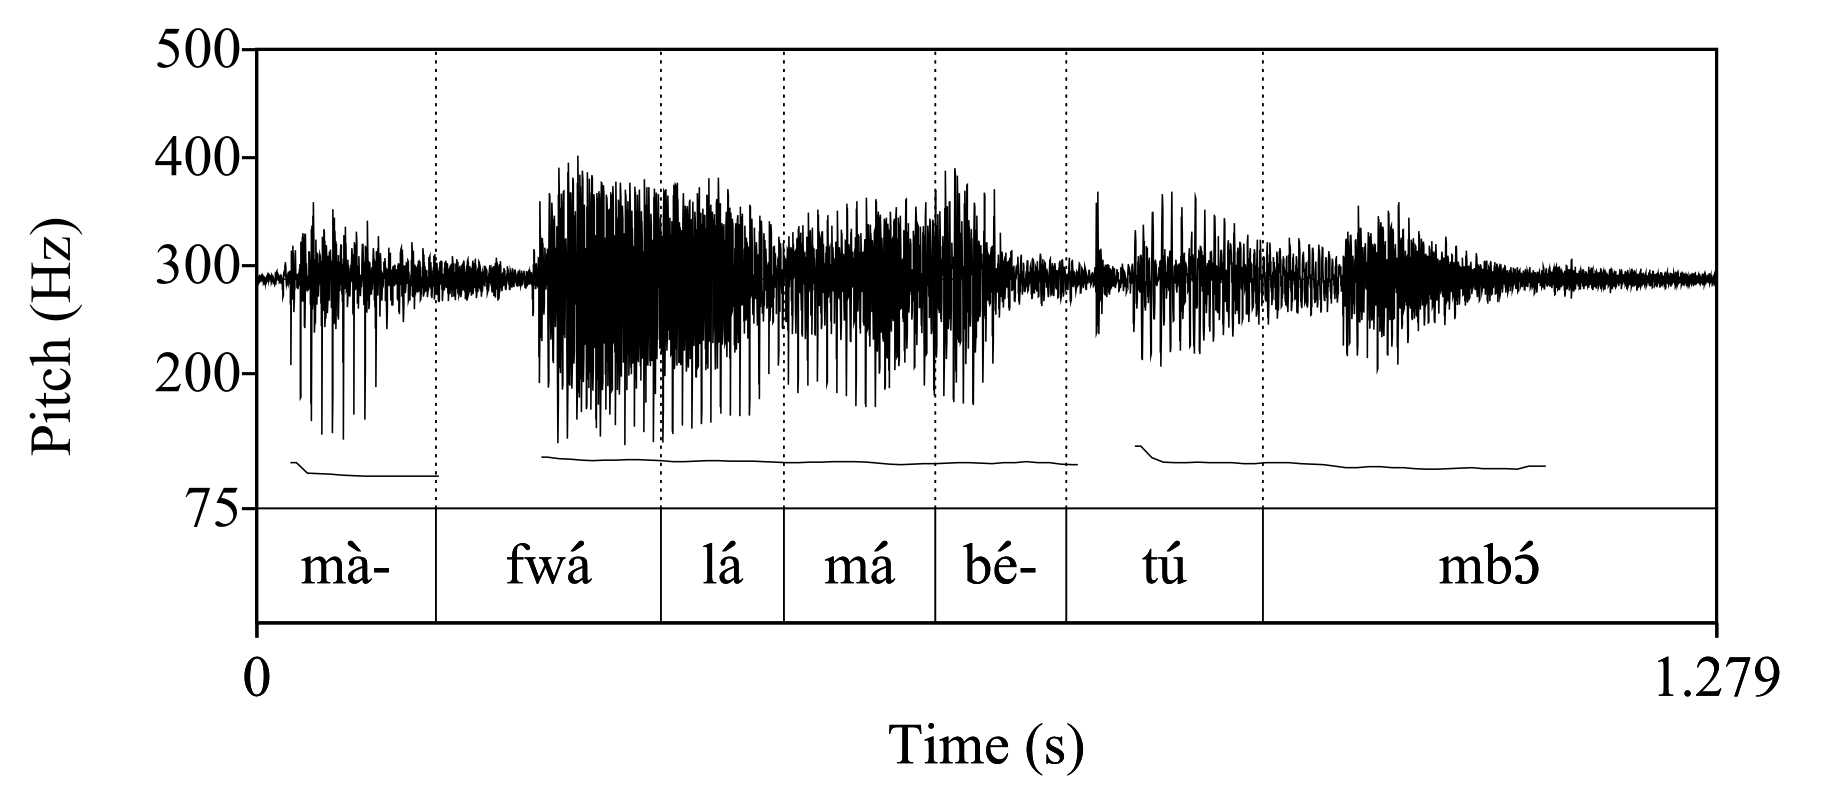
\includegraphics[width=\textwidth]{figures/H-plateau.jpg}
\caption{Pitch in HTS within the nominal domain}
\label{Fig:pitchHTS}
\end{figure}

H tone lowering may occur towards stem final positions if a H is preceded by a L, as shown in Figure \ref{Fig:FinalLow}. The final H in the N + N construction {\itshape bà-bwálɛ̀ bá bá-ntɛ̀mbɔ́} `the parents of the younger siblings' is lower than the H tones on all other H syllables.  This, however, seems to be a phonetic realization phenomenon rather than a phonological rule. The final H is affected both by the preceding L and its utterance final position, lacking the energy to be produced with the same pitch as the preceding H tones.


\begin{figure} 
\centering
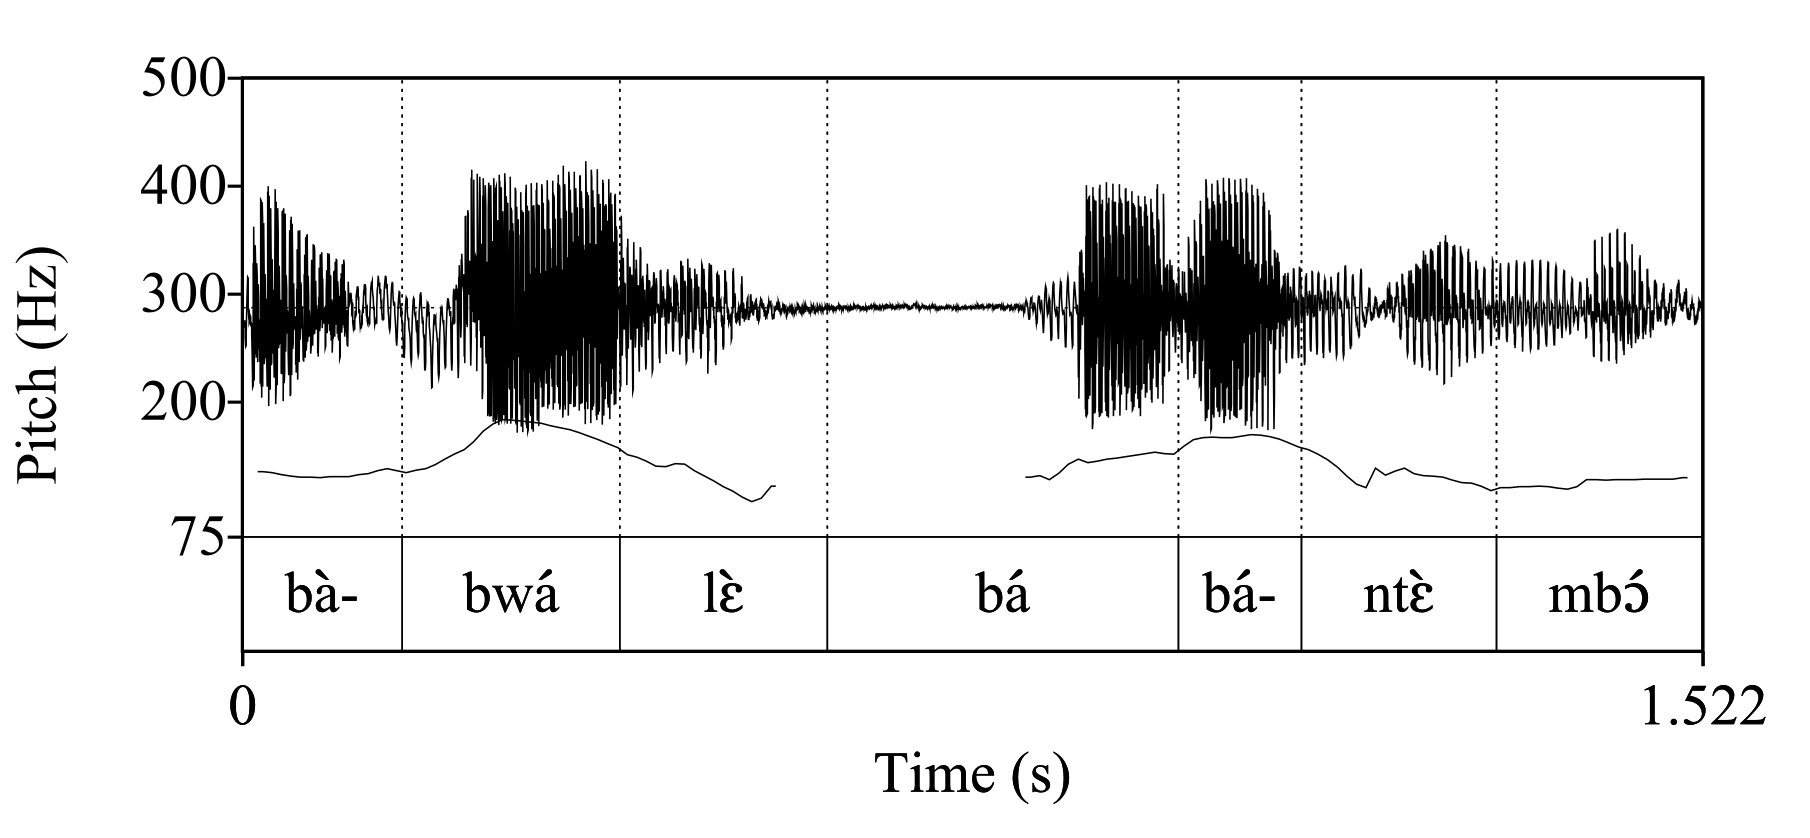
\includegraphics[width=\textwidth]{figures/Final-lowering.jpg}
\caption{Phonetic pitch lowering of final H after L}
\label{Fig:FinalLow}
\end{figure}






The second grammatical environment where HTS onto CV noun class prefixes occurs is with the floating object linking H tone, as discussed in detail in \sectref{sec:OBJTone} and \sectref{sec:HLinker}. The fact that the object linking H tone is indeed only realized on toneless TBUs, is shown in (\ref{HTSM}). The nominal object {\itshape ntúà} `mango' in (\ref{HTSM1}) lacks an overt noun class prefix and thus the object linking H tone does not attach. Also phonetically, there is no change in the tonal pattern of the noun stem that could indicate the presence of the H tone. 

\begin{exe} 
\ex\label{HTSM}
\begin{xlist}
\ex\label{HTSM1}
  \glll    mɛ́ wúmbɛ́ dè ntúà  \\
	    mɛ-H wúmbɛ-H dè ntúà \\ 
              1\textsc{sg}-PRES want-R eat $\emptyset$7.mango   \\
    \trans `I want to eat a/the mango.'
\ex\label{HTSM2}
  \glll    mɛ́ wúmbɛ́ dè {\bfseries má}-ntúà  \\
	    mɛ-H wúmbɛ-H dè H-ma-ntúà \\ 
              1\textsc{sg}-PRES want-R eat OBJ.LINK-ma6-mango   \\
    \trans `I want to eat (the) mangos.'
\end{xlist}
\end{exe}

\noindent  In contrast, the nominal object {\itshape mantúà} `mangos' in (\ref{HTSM2}) has a CV noun class prefix which takes the object linking H tone.

Not every H tone preceding a toneless CV noun class prefix licences HTS. H tones that are part of a preceding lexical stem, as the H verb in (\ref{HTSV}), do not spread onto the toneless TBU, which surfaces L. The object linking H tone is absent in this example because the noun phrase following the verb is not an argument, but an adjunct.

\begin{exe} 
\ex\label{HTSV}
\begin{xlist}
\ex\label{HTSV1}
  \glll    mɛ̀ kwé {\bfseries mà}fû mábáà  \\
	    mɛ kwê-H ma-fû má-báà \\ 
              1\textsc{sg}.PST1 fall-PST ma6-day 6-two  \\
    \trans `I fell two days ago.'
\ex\label{HTSV2}
  \glll    *mɛ̀ kwé {\bfseries má}fû mábáà  \\
	    mɛ kwê-H ma-fû má-báà \\ 
              1\textsc{sg}.PST1 fall-PST ma6-day 6-two  \\
    \trans `I fell two days ago.'
\end{xlist}
\end{exe}

The same is true for a second object whose toneless CV noun class prefix follows a H nominal stem, as in (\ref{HTSN}). The object linking H tone only occurs after the (lexical) verb and only attaches to the object that directly follows it. A second object surfaces with a L CV noun class prefix, even if the preceding nominal stem ends in a H tone.


\begin{exe} 
\ex\label{HTSN}
\begin{xlist}
\ex\label{HTSN1}
  \glll    á dílɛ́sɛ́ bésíŋgí {\bfseries mà}bèlé  \\
	    a-H dílɛsɛ-H H-be-síŋgí ma-bèlé \\ 
             1-PRES feed-R OBJ.LINK-be8-squirrel ma6-kola.nut  \\
    \trans `S/he feeds the squirrels kola nuts.'
\ex\label{HTSN2}
  \glll    *á dílɛ́sɛ́ bésíŋgí {\bfseries má}bèlé  \\
	    a-H dílɛsɛ-H H-be-síŋgí ma-bèlé \\ 
             1-PRES feed-R OBJ.LINK-be8-squirrel ma6-kola.nut  \\
    \trans `S/he feeds the squirrels kola nuts.'
\end{xlist}
\end{exe}



The object linking H tone can also attach to a verbal plural marker {\itshape ŋga}, as it constitutes another morpheme that is underlyingly toneless and thus capable of hosting the H tone.
HTS onto the verbal plural marker is generally restricted to specific grammatical environments for the reason that this marker only occurs in a few positions. Testing grounds for HTS are limited to a preceding HL pattern with imperative verbs and the preceding H tone of the negative auxiliary {\itshape tí}.  These are described with examples in \sectref{sec:nga}. To summarize the overall findings, {\itshape ŋga} follows an  imperative verb form that characteristically carries a final HL pattern. If {\itshape ŋga} is intonation phrase final, it surfaces L, as in (\ref{impP1}). If {\itshape ŋga} is not phrase final, the verbal marker hosts a potential object linking H tone which it  `steals' from a nominal object, as in (\ref{impP2}). This example also shows that the H tone cannot spread further onto other toneless TBUs. The underlyingly toneless CV noun class prefix of {\itshape mantúà} `mangos' has to surface L.


\begin{exe}
\ex\label{impP}
\begin{xlist}
\ex \label{impP1}
  \glll gyàgâ {\bfseries ŋgà} \\
         gyàgâ ŋga \\
         buy.IMP PL\\
    \trans `Buy (pl.)!' 
\ex\label{impP2}
  \glll gyàgâ {\bfseries ŋgá} màntúà \\
         gyàgâ H-ŋga ma-ntúà \\
         buy.IMP OBJ.LINK-PL ma6-mango\\
    \trans `Buy (pl.) mangos!' 
\end{xlist}
\end{exe}


The verbal marker also follows the negative auxiliary {\itshape tí}, which is then followed by a lexical non-finite verb. In this case, {\itshape ŋga} always takes the H tone from the preceding auxiliary, as illustrated in (\ref{impP3}). 

\begin{exe}
\ex\label{impP3}
  \glll tí {\bfseries ŋgá} gyàgà mántúà \\
         tí ŋga gyàga H-ma-ntúà \\
         NEG.R PL buy OBJ.LINK-ma6-manngo\\
    \trans `Don't (pl.) buy mangos!' 
\end{exe}


\noindent Given these positional restrictions, investigating the tonal behavior of {\itshape ŋga} following, for instance, a lexical H tone, is therefore impossible.






\subsubsection{High tone spreading to the left}
\label{sec:HTSl}

HTS in verbs  differs from other instances of HTS in that the spreading goes to the left rather than to the right. The tone that attaches to the right of a verb can be viewed as a melodic tone in the sense of \citet{odden2014} and \citet{marlo2018} and is either a H or a HL, depending on the inflectional category it marks. A grammatical floating H tone encodes past tenses (\sectref{sec:GramTM}) and/or realis mood (\sectref{sec:SynH}). A verb final HL tone, which spreads H to the left in case there is a second toneless TBU, marks imperative and subjunctive categories (\sectref{sec:imp} and \sectref{sec:opt}). The origin of HTS in verbs thus differs from the sources of HTS in nouns and verbal plural markers.

Regardless of the function of the attaching tones, phonologically tones can only spread across underlyingly toneless TBUs in verbs. These include second and third syllables, while first syllables are always specified for H or L. This is illustrated in the autosegmental representation in (\ref{Tonegyaga}) where a floating H tone (either past tense or realis mood marking) attaches to the second, toneless syllable of the verb {\itshape gyàga} `buy', while the first syllable keeps its lexical L tone.

\begin{exe} \ex \label{Tonegyaga}
\begin{minipage}[t]{0.13\textwidth}
$\xymatrix@1@C=0pt{gy&a\ar@{-}[d]& g & a&&&\\
&L  &   &  &&&}$
\end{minipage}
\begin{minipage}[t]{0.07\textwidth}
$\rightarrow$
\end{minipage}
\begin{minipage}[t]{0.13\textwidth}

$\xymatrix@1@C=0pt{gy&a\ar@{-}[d]& g & a\ar@{--}[d]&&&\\
&L  &   & *+<7pt>+[Fo]{H} &}
$
\end{minipage}
\begin{minipage}[t]{0.07\textwidth}
$\rightarrow$
\end{minipage}
\begin{minipage}[t]{0.1\textwidth}

$\xymatrix@1@C=0pt{gy&a\ar@{-}[d]& g & a\ar@{-}[d]&&&\\
&L  &   & H &}
$
\end{minipage}
\end{exe}

If a H attaches to a trisyllabic verb stem, as with the verb {\itshape vìdega} `turn' in (\ref{Tonevidega}), the H attaches to the rightmost toneless TBU and the spreads to the left to the second verb syllable. Again, the first syllable keeps its lexical tone.

\begin{exe} \ex \label{Tonevidega}
%$\xymatrix@1@C=0pt{gy&a\ar@{-}[d]& g & a&&&\\ &L  &   & { } & $
\begin{minipage}[t]{0.2\textwidth}
$\xymatrix@1@C=0pt{v&i\ar@{-}[d]&d&e       & g   & a      &&&\\
                                     &L               &  &  &      &   &&&}$
\end{minipage}
\begin{minipage}[t]{0.07\textwidth}
$\rightarrow$
\end{minipage}
\begin{minipage}[t]{0.2\textwidth}

$\xymatrix@1@C=0pt{v&i\ar@{-}[d]&d&e\ar@{--}[1,2]& g & a\ar@{--}[d]&&&\\
&L &   &  && *+<7pt>+[Fo]{H} }$
\end{minipage}
\begin{minipage}[t]{0.07\textwidth}
$\rightarrow$
\end{minipage}
\begin{minipage}[t]{0.2\textwidth}

$\xymatrix@1@C=0pt{v&i\ar@{-}[d]& d & e\ar@{-}[1,2]&g&a\ar@{-}[d]&\\
&L  &   & & & H}
$
\end{minipage}
\end{exe}


If the first verb syllable is H, the surface tonal pattern ends up with a sequence of H tones, as illustrated in (\ref{Toneviyala}) for the verb {\itshape víyala} `touch'. 


\begin{exe} \ex \label{Toneviyala}
%$\xymatrix@1@C=0pt{gy&a\ar@{-}[d]& g & a&&&\\ &L  &   & { } & $
\begin{minipage}[t]{0.2\textwidth}
$\xymatrix@1@C=0pt{v&i\ar@{-}[d]&y&a       & l   & a      &&&\\
                                     &H               &  &  &      &   &&&}$
\end{minipage}
\begin{minipage}[t]{0.07\textwidth}
$\rightarrow$
\end{minipage}
\begin{minipage}[t]{0.2\textwidth}

$\xymatrix@1@C=0pt{v&i\ar@{-}[d]&y&a\ar@{--}[1,2]& l & a\ar@{--}[d]&&&\\
&H &   &  && *+<7pt>+[Fo]{H} }$
\end{minipage}
\begin{minipage}[t]{0.07\textwidth}
$\rightarrow$
\end{minipage}
\begin{minipage}[t]{0.2\textwidth}

$\xymatrix@1@C=0pt{v&i\ar@{-}[d]& y & a\ar@{-}[1,2]&l&a\ar@{-}[d]&\\
&H  &   & & & H}
$
\end{minipage}
\end{exe}



\noindent Just as in HTS to the right, there is no OCP rule prohibiting such sequences of H tones. In (\ref{HTS}), for instance, a realis marking H attaches to the finite verb and spreads across its toneless TBUs, while an object linking H attaches to the following noun class prefix, resulting in a sequence of five H tones.


\begin{exe} 
\ex\label{HTS}
  \glll     à swásɛ́lɛ́ bápándyɛ̀ \\
	a swásɛlɛ-H H-ba-pándyɛ̀ \\	
            1.PST1 dry-R OBJ.LINK-ba2-plate     \\
    \trans `S/he dried the plates.'
\end{exe}

\noindent As Figure \ref{Fig:NoOCP} shows, all five H tones are at the same pitch level throughout the utterance so that potential downstep phenomena can be ruled out.


\begin{figure} 
\centering
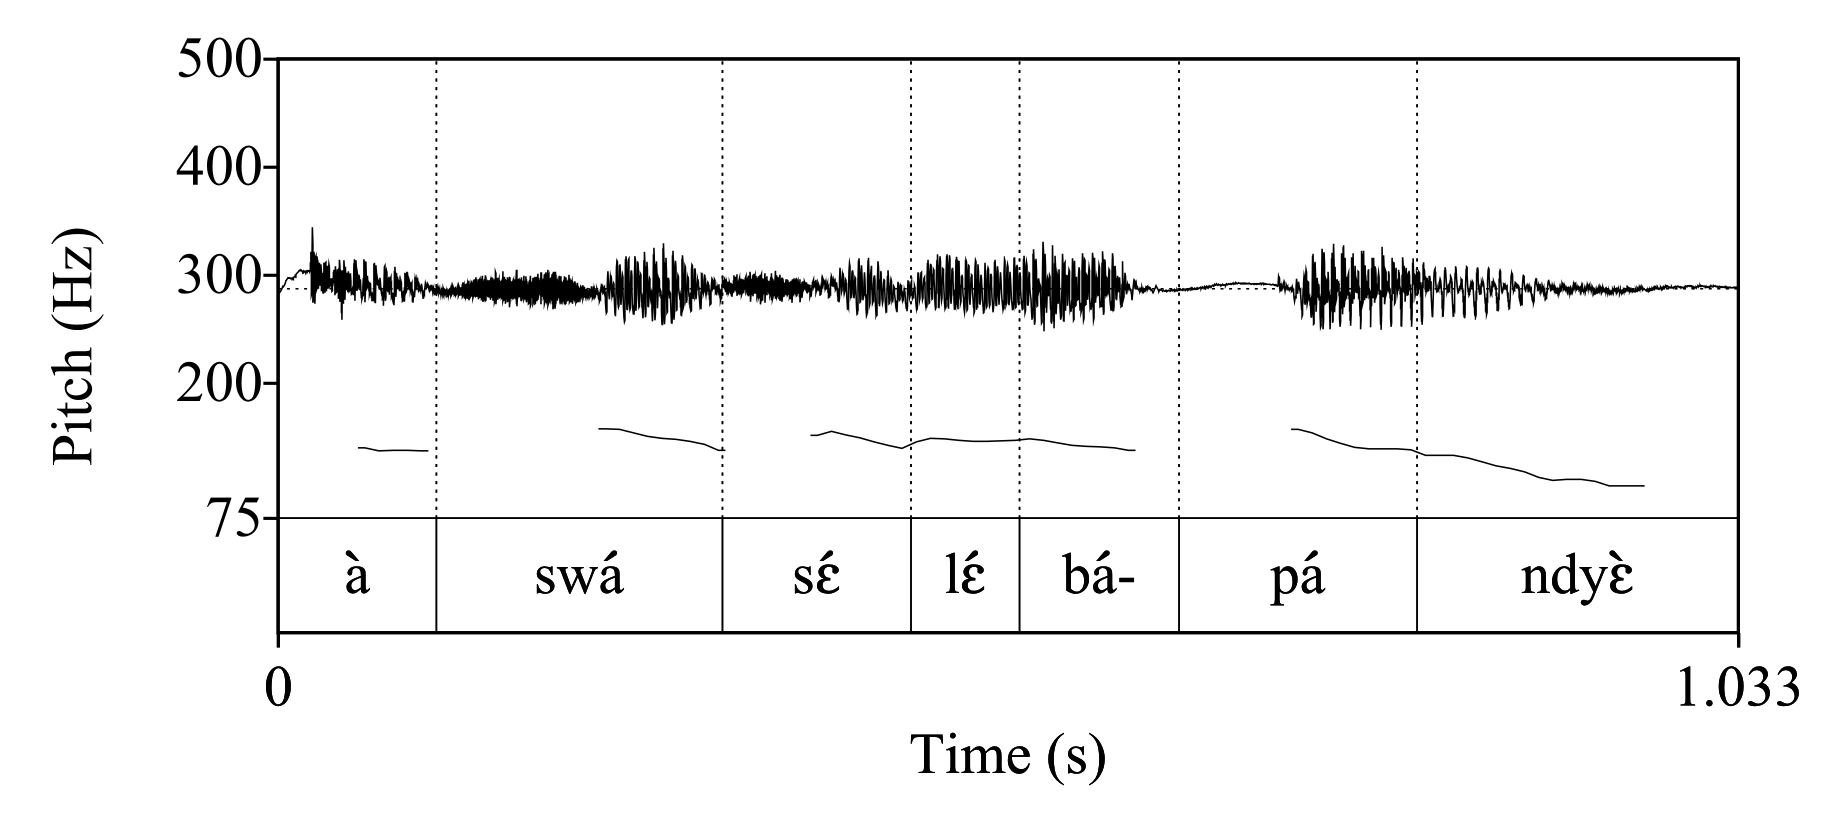
\includegraphics[width=\textwidth]{figures/No-OCP.jpg}
\caption{Pitch level of H sequence}
\label{Fig:NoOCP}
\end{figure}

In addition to floating H tones that attach to the right side of verbs, also HL melodies attach to verb stems, marking categories such as imperative and subjunctive. In bisyllabic verb stems, the HL melody is realized on the final toneless TBU, as shown in (\ref{TonegyagaHL}).

\begin{exe} \ex \label{TonegyagaHL}
\begin{minipage}[t]{0.13\textwidth}
$\xymatrix@1@C=0pt{gy&a\ar@{-}[d]& g & a&&&\\
&L  &   &  &&&}$
\end{minipage}
\begin{minipage}[t]{0.07\textwidth}
$\rightarrow$
\end{minipage}
\begin{minipage}[t]{0.13\textwidth}

$\xymatrix@1@C=0pt{gy&a\ar@{-}[d]& g & a\ar@{--}[d]&&&\\
&L  &   & *+<7pt>+[Fo]{HL} &}
$
\end{minipage}
\begin{minipage}[t]{0.07\textwidth}
$\rightarrow$
\end{minipage}
\begin{minipage}[t]{0.1\textwidth}

$\xymatrix@1@C=0pt{gy&a\ar@{-}[d]& g & a\ar@{-}[d]&&&\\
&L  &   & HL &}
$
\end{minipage}
\end{exe}

In case there is a second toneless TBU, as in (\ref{TonevidegaHL}), only the H of the HL melody spreads to the left, while the final TBU remains HL.



\begin{exe} \ex \label{TonevidegaHL}
%$\xymatrix@1@C=0pt{gy&a\ar@{-}[d]& g & a&&&\\ &L  &   & { } & $
\begin{minipage}[t]{0.2\textwidth}
$\xymatrix@1@C=0pt{v&i\ar@{-}[d]&d&e       & g   & a      &&&\\
                                     &L               &  &  &      &   &&&}$
\end{minipage}
\begin{minipage}[t]{0.07\textwidth}
$\rightarrow$
\end{minipage}
\begin{minipage}[t]{0.2\textwidth}

$\xymatrix@1@C=0pt{v&i\ar@{-}[d]&d&e\ar@{--}[1,2]& g & a\ar@{--}[d]&&&\\
&L &   &  && *+<7pt>+[Fo]{HL} }$
\end{minipage}
\begin{minipage}[t]{0.07\textwidth}
$\rightarrow$
\end{minipage}
\begin{minipage}[t]{0.2\textwidth}

$\xymatrix@1@C=0pt{v&i\ar@{-}[d]& d & e\ar@{-}[d]&g&a\ar@{-}[d]&\\
&L  &   & H& & HL}
$
\end{minipage}
\end{exe}

I take this tonal behavior as an argument to posit tonal attachment to the right with leftwards spreading rather than assuming a tonal attachment to the first toneless TBU with spread to the right. This way, the processes for both attaching tonal melodies, H and HL, are the same: the melody attaches to the right and H spreads leftwards. If rightwards spreading was the case, I would need an additional rule that specifies when a H tone lowers to HL on the final toneless syllable or when it remains H. This view is further in line with analyses of other languages of the area. \citet{marlo2014}, for instance, assume the attachment of one of six inflectional melodies to the right of Bakweri (Bantu A22) verbs, stating that melody initial H spreads leftwards.




\subsubsection{L detachment in monosyllabic L verb stems}
\label{sec:ToneDetach}

In tonal inflection of verbs for various tense, aspect, mood, and polarity categories, the processes of tonal attachment and spreading as described for bi- and trisyllabic verb stems above do not work for monosyllabic verb stems since these are already specified for tone and there are no toneless TBUs to which a tonal melody could attach and/or spread. Nevertheless, the same inflectional melodies surface on monosyllabic stems as on stems that have toneless TBUs. For monosyllabic L verb stems, I assume tonal detachment of the lexical tone which is then replaced by the inflectional tone melody, either H or HL.
 
Monosyllabic L verb stems take a H in past tenses (\ref{Detachde2})  and in the realis mood (\ref{Detachde3}).


\begin{exe} 
\ex\label{Detachde}
\begin{xlist}
\ex\label{Detachde1} 
  \glll     mɛ́ d{\bfseries è} \\
	mɛ-H dè \\	
            1\textsc{sg}-PRES eat     \\
    \trans `I eat.'
\ex\label{Detachde2}
  \glll    mɛ̀ d{\bfseries é} \\
	mɛ dè-H \\	
            1\textsc{sg}.PST1 eat-PST     \\
    \trans `I ate.'
\ex\label{Detachde3} 
  \glll     mɛ́ d{\bfseries é} tɛ́ɛ̀ \\
	mɛ-H dè-H tɛ́ɛ̀ \\	
            1\textsc{sg}-PRES eat-R now     \\
    \trans `I eat now.'
\end{xlist}
\end{exe}

In order to explain how a H in monosyllabic L verb stems surfaces, simple H attachment and/or spreading is not enough. A specified L must either be deleted before the H can attach or be featurally changed. For the sake of consistency with HTS of bi- and trisyllabic verb stems, I propose that a L in monosyllabic verb stems gets detached, as shown in (\ref{Tonede}), and then replaced by the inflectional H.


\begin{exe} \ex \label{Tonede}
\begin{minipage}[t]{0.07\textwidth}
$\xymatrix@1@C=0pt{d&e\ar@{-}[d] &  & &&&\\
&L  &   & { } &}
$ 
\end{minipage}
\begin{minipage}[t]{0.07\textwidth}
$\rightarrow$
\end{minipage}
\begin{minipage}[t]{0.1\textwidth}
$\xymatrix@1@C=0pt{d&e\ar@{-}[d]|= \ar@{--}[1,3]&  & &&&\\
&L  &   & { } &*+<7pt>+[Fo]{H}}
$

\end{minipage}
\begin{minipage}[t]{0.07\textwidth}
$\rightarrow$
\end{minipage}
\begin{minipage}[t]{0.1\textwidth}
$\xymatrix@1@C=0pt{d&e\ar@{-}[d] &  & &&&\\
&H  &   & { } &}
$ 
\end{minipage}
\end{exe}

The same is true for a HL melody attaching to a monosyllabic L verb, as illustrated in (\ref{TonedeHL}).


\begin{exe} \ex \label{TonedeHL}
\begin{minipage}[t]{0.07\textwidth}
$\xymatrix@1@C=0pt{d&e\ar@{-}[d] &  & &&&\\
&L  &   & { } &}
$ 
\end{minipage}
\begin{minipage}[t]{0.07\textwidth}
$\rightarrow$
\end{minipage}
\begin{minipage}[t]{0.1\textwidth}
$\xymatrix@1@C=0pt{d&e\ar@{-}[d]|= \ar@{--}[1,3]&  & &&&\\
&L  &   & { } &*+<7pt>+[Fo]{HL}}
$

\end{minipage}
\begin{minipage}[t]{0.07\textwidth}
$\rightarrow$
\end{minipage}
\begin{minipage}[t]{0.1\textwidth}
$\xymatrix@1@C=0pt{d&e\ar@{-}[d] &  & &&&\\
&HL  &   & { } &}
$ 
\end{minipage}
\end{exe}







\subsubsection{H lowering in monosyllabic H verb stems}
\label{sec:ToneLower}

While all other verb stems (monosyllabic L as well as bi- and trisyllabic stems) show the same tonal surface patterns on the final syllable, monosyllabic H stems deviate from this pattern, as shown in Table \ref{Tab:Vpattsurf}.\footnote{The three environment categories in Table \ref{Tab:Vpattsurf} each subsume different grammatical categories in which this surface form is used. The citation form comprises a verb uttered in isolation as well as the non-finite form, and present, future, and inchoative tense-mood verb forms. The inflectional melody 1, a final H, is used in past tenses and for marking realis mood. The inflectional melody 2, a final HL, marks imperative and subjunctive. The grammatical functions of verb tones and their interaction with tonal melodies of subject-tense-aspect-mood-polarity markers are discussed in \chapref{sec:TAM}.}


\begin{table} 
\centering
\begin{tabular}{l|ll}
Environment  			& 	General pattern		& Monosyllabic H \\
 \midrule
Citation form 			& 	L 				&  HL		\\
Inflectional melody 1		& 	H 				& H 			\\
Inflectional melody 2 	& 	HL 				& HL 		\\
 \midrule
\end{tabular}
\caption{Surface patterns of verb stem final syllables}
\label{Tab:Vpattsurf}
\end{table}



As explained in \sectref{sec:HTSl} and \sectref{sec:ToneDetach}, the tonal processes that are involved in arriving at the surface tonal melodies of final verb syllables differ between monosyllabic L verb stems and verb stems with more than one syllable which include toneless TBUs as well. Monosyllabic H stems, however, already pose an exception to the general surface pattern as there is a syncretism between forms in isolation and the HL inflectional melody.

The question how the HL surface tone of monosyllabic verb citation forms is derived presents different analytic possibilities which I evaluate in terms of likelihood. I propose to view these verbs underlyingly as monosyllabic H verbs which get lowered to a falling HL tone in the citation form categories.
(\ref{Tonekwe}) shows the autosegmental representation of the final lowering in citation form categories (non-finite, present, future, and inchoative) of monosyllabic H verb stems. A lowering L attaches to an underlying monosyllabic H verb stem, resulting in a HL surface form.

\begin{exe} \ex \label{Tonekwe}
\begin{minipage}[t]{0.07\textwidth}
$\xymatrix@1@C=0pt{kw&e\ar@{-}[d] &  & &&&\\
&H  &   & { } &}
$ 
\end{minipage}
\begin{minipage}[t]{0.07\textwidth}
$\rightarrow$
\end{minipage}
\begin{minipage}[t]{0.1\textwidth}
$\xymatrix@1@C=0pt{kw&e\ar@{-}[d] \ar@{--}[1,3]&  & &&&\\
&H  &   & { } &*+<7pt>+[Fo]{L}}
$

\end{minipage}
\begin{minipage}[t]{0.07\textwidth}
$\rightarrow$
\end{minipage}
\begin{minipage}[t]{0.1\textwidth}
$\xymatrix@1@C=0pt{kw&e\ar@{-}[d] \ar@{-}[1,3]&  & &&&\\
&H  &   & { } &L}
$
\end{minipage}
\end{exe}


\noindent This is the reason why there are, on the surface, no monosyllabic H non-finite verb forms, they all surface as HL.\footnote{See the distribution of level and contour tones in \sectref{sec:Level} and \sectref{sec:Contour}.} \citet[230]{renaud76} addresses this phenomenon, subsuming it under a general rule of /  ́/ $\rightarrow$ /  ̂/ at the end of a syntagm. This rule, however, is not context sensitive, neglecting cases of syntagm final melodic H, for instance for past tense forms.\todo[2806]{alignment of tone placement in tone rule, diacritics not centered between slashes}

The representation that follows for glossing is exemplified in (\ref{Detachkwe}) for all tonal melodies that attach. For citation form categories such as the present in (\ref{Detachkwe1}), the underlying monosyllabic H stem is lowered to HL by a L. For the inflectional melody 1 with a H in (\ref{Detachkwe2}), the verb just surfaces with its underlying H form. In (\ref{Detachkwe3}), the HL inflectional melody 2 overrides the underlying H, resulting in a surface pattern that is identical to citation form categories. 

\begin{exe} 
\ex\label{Detachkwe}
\begin{xlist}
\ex\label{Detachkwe1} 
  \glll     mɛ́ kw{\bfseries ê} \\
	mɛ-H kwé-L \\	
            1\textsc{sg}-PRES fall-CF     \\
    \trans `I fall.'
\ex\label{Detachkwe2}
  \glll    mɛ̀ kw{\bfseries é} \\
	mɛ kwé-H \\	
            1\textsc{sg}.PST1 fall-PST     \\
    \trans `I fell.'
\ex\label{Detachkwe3}
  \glll   kw{\bfseries ê} \\
	kwé-HL \\	
            fall-IMP     \\
    \trans `Fall!'
\end{xlist}
\end{exe}

Since the final lowering of citation form categories in monosyllabic H verb stems is purely phonological  and does not seem to carry any grammatical function, unlike the inflectional tonal melodies, I do not represent the phonological lowering rule in my glossing in the following chapters and appendices.  In order to be consistent with the other verb patterns and to transparently track the attachment of inflectional melodies, I use the glosses as in (\ref{Detachkweb}). The HL citation form will appear in the underlying form line (the second line) and possibly take inflectional melodies as in (\ref{Detachkwe2b}). It should be kept in mind though that, phonologically, the underlying form of HL monosyllabic verb stems is in fact H.


\begin{exe} 
\ex\label{Detachkweb}
\begin{xlist}
\ex\label{Detachkwe1b} 
  \glll     mɛ́ kw{\bfseries ê} \\
	mɛ-H kwê \\	
            1\textsc{sg}-PRES fall     \\
    \trans `I fall.'
\ex\label{Detachkwe2b}
  \glll    mɛ̀ kw{\bfseries é} \\
	mɛ kwê-H \\	
            1\textsc{sg}.PST1 fall-PST     \\
    \trans `I fell.'
\end{xlist}
\end{exe}

There are two other possibilities how to analyze the surface HL form on monosyllabic verb stems. First, HL  could be the underlying form, just as monosyllabic L verbs are underlyingly specified for L. This would mean, however, that there is a contrast between L and HL verb roots for monosyllabic stems, while polysyllabic stems have a lexical contrast of H and L. Another argument against this analysis comes from the distribution of contour tones in Gyeli which are generally only found in nouns, but not in verb stems. Monosyllabic stems would be the only exception, but a H tone contrast is more likely.

Second, one may also posit a H vs.\ toneless distinction for monosyllabic verb stems. Under this analysis, the citation form categories would all carry a final L tone which surfaces L for toneless monosyllabic as well as for polysyllabic verb stems and HL for underlying monosyllabic H stems. While a H vs.\ toneless analysis generally makes sense in many Bantu languages, it does not quite fit the patterns of bi- and trisyllabic verb stems in Gyeli whose first syllables are clearly specified for either H or L, but not toneless. I therefore do not assume any lexical toneless roots (first syllables) for Gyeli.




\section[Discussion: Bantu A80 phonology]{Discussion: Gyeli phonology within Bantu A80}
\label{sec:PhonA80}

Having described consonants, vowels, syllables and tones in Gyeli, I conclude this chapter by comparing Gyeli phonology to other Bantu A80 languages and thus locating Gyeli within this language family. For comparative data, I refer to \citet{cheucle2014} whose valuable thesis is based on her own fieldwork on Bekwel as well as an assemblage of data by various authors. Her comparison includes Bekwel, Bekol, Konzime, Makaa, Mpiemo, Kwasio, Njyem, and Shiwa which she uses to reconstruct Proto-A80.\footnote{These are the languages that are sufficiently described to allow for  systematic comparison. A few A90 languages may arguably be considered as more closely related to A80 and should thus be included in such a comparison, but this exceeds the frame of this work.} The data show that Gyeli possesses many properties that are found in the A80 group. At the same time, it is most closely related to Kwasio and to Shiwa and possibly Mpiemo, as can be seen from many characteristics these languages have in common and which are absent in the other languages.

\paragraph{Consonants} Gyeli's consonant inventory is quite close to the Proto-A80 one as reconstructed by \citet[432]{cheucle2014}. Its main difference concerns the series of fricatives for which the author proposes /s/ as the only fricative in the Proto language, while Gyeli's fricative inventory has expanded, synchronically comprising /f/, /v/, /s/, and /z/.

 According to \citet[335]{cheucle2014}, all compared A80 languages have a series of bilabial, alveolar, palatal and velar stops, both voiced and voiceless.\footnote{\citet[335]{cheucle2014} classifies /tʃ/ or /ts/ as well as /dj/ or /dʒ/ in the literature as palatal /c/ and /ɟ/. In Gyeli, they correspond to the affricates /tʃ/ and /dʒ/.} Gyeli clusters more closely with Kwasio and Shiwa though in three respects. First, also in Kwasio the use of /g/ is highly restricted. Second, Kwasio and Shiwa are the only two other A80 languages that feature fricative clusters as in Gyeli such as /pf/, /bv/, /kf/, and /gv/. Third, Shiwa is the only other language, with Gyeli, that allows for voiceless stops in C\textsubscript{2} while all other A80 languages exclusively allow voiced plosives in this position (Cheucle 2014: 340).

The distribution of fricatives among A80 languages is synchronically more varied. \citet[342]{cheucle2014} lists six possible fricatives that may occur: /f/, /v/, /s/, /z/, /ʃ/, and /ʒ/. Gyeli features the first four of them, but lacks the latter two. No other language displays the same distribution. The most similar distribution is found in Konzime which has /s/ and /z/, but only a restricted occurrence of /f/ and /v/, and Kwasio with the same phonemes, just that /f/, /v/, and /z/ are rather limited.

Other consonants are less varied across A80, all featuring nasals /m/, /n/, and /ɲ/. Also /l/, /w/, and /j/ are found in all languages. They all feature NC clusters, but for many languages (Konzime, Njyem, Kwasio, and Shiwa), their phonological status is not clear, according to \citet[348]{cheucle2014}. Nevertheless, all languages, including Gyeli, have both prenasalized voiced and voiceless obstruents, except for Kwasio and Shiwa which are otherwise most similar to Gyeli in other charateristics.


\paragraph{Vowels} \citet[324]{cheucle2014} states that A80 languages differ significantly in their number of vowels, ranging between 5 and 11, as well as in their vowel quality. The vowels that all languages under investigation have in common are /i/, /u/, /ɛ/, and /a/. Differences concern thus mostly the mid vowels. Gyeli displays the same 7-vowel system as Bekwel and Mpiemo, comprising /i/, /u/, /e/, /o/, /ɛ/, /ɔ/, and /a/. \citet[389]{cheucle2014} reconstructs this same vowel system for Proto-A80 which means that Gyeli, Bekwel and Mpiemo are the most conservative languages within the A80 group, at least with respect to their vowels.

It is possible that languages such as Gyeli and potentially Mpiemo are currently losing /e/ and /o/ as contrastive phonemes. This hypothesis is supported by the special status of these vowels in Gyeli concerning the small space in the vowel plot and the low frequency, as discussed in \sectref{sec:CardVowels}. Other A80 languages, according to \citet[324-325]{cheucle2014}, support this assumption further since most of them have lost a phonemic vowel in comparison with the seven vowel system of Proto-A80.  In Shiwa and Kwasio, /e/ and /o/ are variants of /ɛ/ and /ɔ/, so there seems to be a tendency to dispense with the higher rather than the lower mid vowels. Also, the trend is to lose vowels rather than expanding the vowel inventory to a nine vowel system, which would be a possible route of innovation.

Contrastive vowel length is found in most A80 languages, as it is in Gyeli. In Gyeli's closest related languages Mpiemo, Kwasio, and Shiwa, however, vowel length has not been analyzed as being phonemic by the authors, as \citet[327]{cheucle2014} points out. In Proto-A80, vowel length is not distinctive. \citet[395-396]{cheucle2014} reconstructs the origin of synchronic distinctive vowel length as final nasal consonants or syllables with /b/ as their onset, which have been lost in some languages and replaced by long vowels.

Gyeli seems to have a special status as to nasal vowels within A80. Only Makaa has two nasal vowels /õ/ and /ɛ̃/ while nasal vowels are regarded as contextual in the other languages under investigation, being conditioned by following velar nasals (Cheucle 2014: 329, 397).

Vowel sequences or diphthongs are attested in Konzime, Njyem, Mpiemo, Kwasio, and Shiwa, as summarized by \citet[330]{cheucle2014}. Just as in Gyeli, they occur canonically in monosyllabic stems, but differ in their number and vowel quality. The sequence/diphthong /uo/ (or /uɔ/), for instance, is only attested in Gyeli, Konzime, Kwasio, and Shiwa.

A feature that is absent in Gyeli, but widespread in other A80 languages is an epenthetic vowel. \citet[332]{cheucle2014} specifies that this is most often a schwa, at least for the languages Bekol, Makaa, Konzime, and Bekwel.

\paragraph{Syllables} \citet[319]{cheucle2014} states that A80 languages are generally characterized by open syllables and a canonical CV type, allowing, however, also other types of syllables, including closed ones. In this, Gyeli differs from the majority of A80 languages in that it  has exclusively open syllables. The only other language with this restriction is Shiwa.

All studied A80 languages allow for complex onsets, including Gyeli. Even though an onset is most frequently occupied by a simple consonant, more complex clusters are allowed. \citet[319]{cheucle2014} distinguishes consonant clusters that include a consonant and a glide, but treats nasal + consonant clusters as well as affricates as phonemic units. Therefore, a comparison of onset complexity and frequency is not possible at this point.

As to syllable structures in prefixes, all languages under investigation allow CV prefixes, according to \citet[322]{cheucle2014}. In terms of other prefix structures, however, they differ. Gyeli shares with Shiwa and Kwasio the feature of not allowing V type nominal prefixes while all other studied A80 languages do. Shiwa and Kwasio, however, feature syllabic nasal prefixes, Gyeli does not. In that, it behaves like Konzime and Njyem which have nasal prefixes which are not syllabic.

\paragraph{Tone} A tonal comparison across A80 languages is limited to lexical tones and even then rather tentative since tone is treated to varying degrees in the literature. Nevertheless, according to \citet[350]{cheucle2014}'s summary of A80 lexical tone, Gyeli behaves as expected, displaying a H and a L level tone as well as HL and LH contour tones, the latter of which may be realized as a mid tone in some languages. The literature does not, however, discuss potentially toneless TBUs. It would be worthwhile to investigate tonal rules and grammatical tone across A80 languages in the future especially since \citet[59]{kisseberth2003} point out that despite a widespread two level tone opposition in Bantu languages, there is considerable variation between Bantu languages and dialects in terms of their tonal systems.

















